%------------------------------------------------------------------------
%                           PDFFIT Users guide
%------------------------------------------------------------------------
% Version:  April 2007
%------------------------------------------------------------------------

\documentclass[11pt]{report}

\usepackage[letterpaper]{geometry}
\geometry{height=8.5in}
\geometry{bottom=1.1in}
\geometry{left=1.1in}
\geometry{right=1.1in}

\usepackage[dvips]{graphicx}
\usepackage{fancyhdr}
\usepackage{floatflt}
\usepackage{tabularx}
\usepackage[round]{natbib}
\usepackage[hang,small,bf]{caption2}
\usepackage{fancyvrb}
\usepackage{scalefnt}
\usepackage{color}
\usepackage{url}

\usepackage[T1]{fontenc}
\usepackage{palatino}

\newcommand{\version}{1.4}

% General page style

\pagestyle{fancy}
\fancyhf{}
\fancyhead[L]{\bfseries \slshape\leftmark}
\fancyhead[R]{\bfseries Users Guide}
\fancyfoot[R]{\bfseries Page \thepage}
\fancyfoot[L]{\bfseries PDFFIT \version}
\renewcommand{\footrulewidth}{0.4pt}
\renewcommand{\headrulewidth}{0.4pt}

% Style for chapter start pages ..

\fancypagestyle{plain} {
  \fancyhf{}
  \fancyhead[R]{\bfseries Users Guide}
  \fancyfoot[L]{\bfseries PDFFIT \version}
  \fancyfoot[R]{\bfseries Page \thepage}
  \renewcommand{\headrulewidth}{0.4pt}
}

% MacVerbatim style for macros

\definecolor{DarkBlue}{rgb}{0.1,0.0,0.5}

\DefineVerbatimEnvironment%
{MacVerbatim}{Verbatim}
{fontfamily=courier,
 fontsize=\scriptsize,
 fontseries=b,
 formatcom=\color{DarkBlue}}

\graphicspath{{pic/}}

\setlength\parindent{0pt}

%------------------------------------------------------------------------

\begin{document}

%------------------------------------------------------------------------
% Title
%------------------------------------------------------------------------

\begin{titlepage}
\begin{flushright}

  \hrule
  \vspace{15mm}
  \textbf{{\scalefont{8} PDFFIT}} \\
  \vspace{15mm}
  \textbf{{\scalefont{4} Users Guide}} \\
  \vspace{10mm}
  \textbf{{\Huge Version  \version}} \\
  \vspace{10mm}

  \hrule
  \vspace{35mm}
  \textbf{written by} \\

  \vspace{5mm}
  \textbf{\Large Thomas Proffen} \\
  Email: tproffen@lanl.gov \\

  \vspace{ 2mm}
  \textbf{\Large Simon Billinge} \\
  Email: billinge@pa.msu.edu \\

  \vspace{12mm}
  \textbf{\Large \url{http://discus.sourceforge.net/}} \\

  \vspace{3mm}
  \hrule

\end{flushright}
\begin{flushright}
  \textit{Document created: \today \\ LA-UR 05-2800}
\end{flushright}

\end{titlepage}

%------------------------------------------------------------------------
% Preface
%------------------------------------------------------------------------

\chapter*{Preface}
\subsection*{Disclaimer}

The {\it PDFFIT} software described in this guide is
provided without warranty of any kind.  No liability is taken for any loss
or damages, direct or indirect, that may result through the use of {\it
PDFFIT}.  No warranty is made with respect to this manual, or the program
and functions therein.  There are no warranties that the programs are free
of error, or that they are consistent with any standard, or that they will
meet the requirement for a particular application.  The programs and the
manual have been thoroughly checked.  Nevertheless, it can not be
guaranteed that the manual is correct and up to date in every detail. This
manual and the {\it PDFFIT} program may be changed without notice.\par

{\it PDFFIT} is intended as a public domain program. It may be used free
of charge.  Any commercial use is, however, not allowed without permission
of the authors.

%------------------------------------------------------------------------

\subsection*{Acknowledgments}

The basic concept of the full profile refinement of the
pair distribution function (PDF) was adapted from the program {\it RESPAR}
written by Simon Billinge \citep{billi;b;lsfd98}. The routines for the
processing of the command language and the FORTRAN style interpreter are
taken from the program package {\it DISCUS} by Reinhard Neder and Thomas
Proffen \citep{prne97}. {\it PDFFIT} is distributed as part of that package
as well as a stand-alone program. The routines for the line editing were
taken from the program GNUPLOT.

%------------------------------------------------------------------------

\subsection*{Using PDFFIT}

Publications of results totally or partially obtained using the program
{\it PDFFIT} should state that {\it PDFFIT} was used and contain the
following reference:

\begin{quote}
  {\sc Proffen, Th. \& Billinge, S.J.L.} (1999) "PDFFIT, a Program
  for Full Profile Structural Refinement of the Atomic Pair
  Distribution Function" {\it J. Appl. Cryst.}, {\bf 32}, 572-575
\end{quote}

%------------------------------------------------------------------------
% Table of contents, List of Tables etc..
%------------------------------------------------------------------------

\tableofcontents

%------------------------------------------------------------------------
% Here all the chapter are included ...
%
% Alter or comment the \includeonly command above to work with the
% complete manual or only certain parts.
%
%------------------------------------------------------------------------

%------------------------------------------------------------------------
% Chapter:  Introduction
%------------------------------------------------------------------------

\chapter{Introduction \label{intro}}
\section{What is PDFFIT ?}

Now you might have installed {\it PDFFIT} and can start it simply
by typing {\tt pdffit} but in case you are not a PDF wizard here is
a little introduction into the PDF method first. For those who hate
to read long manuals, there is section \ref{quick} which shows how
to run a refinement in no time. The remaining users guide explains
the various features of {\it PDFFIT} more detail. \par

The determination of crystal structures is an important part of
chemistry, physics and of course crystallography. Conventional
structure determination is based on the analysis of the
intensities and positions of Bragg reflections which only allows
one to determine the long range {\it average} structure of the
crystal. Only one-body information such as atomic positions, site
occupancies and temperature factors can be extracted.
Determination of the {\it average} structure based on powder
diffraction data is now routinely done using the Rietveld
\citep{rietv;jac69} method which is very similar to the full
profile refinement of the atomic pair distribution function (PDF)
as we will see later. It should be kept in mind that the analysis
of Bragg scattering assumes a prefect long range periodicity of
the crystal. However, many materials are quite disordered and even
more important the key to the deeper understanding of their
properties is the study of deviations from the {\it average}
structure or the study of the {\it local} atomic arrangements.
Deviations from the {\it average} structure result in the
occurrence of diffuse scattering which contains information about
two-body interactions \citep{webu95,fr95}. In recent years the
analysis of diffuse scattering from single crystals as well as
powders using computer simulations have made great advances, in
particular using the Monte Carlo (MC) and the Reverse Monte Carlo
(RMC) technique \citep{webu95,nikemc95,wepr98,prwe98b,prwe97b}.
\par

Another method to reveal the {\it local} structure of a crystal is
the analysis of the PDF. This method is long known in the field of
studying short range order in liquids and glasses but has recently
been applied to crystalline materials \citep{egami;lsfd98,bieg93}.
The PDF is obtained from the powder diffraction data via a simple
Fourier transform of the normalised scattering intensity $S(Q)$:

\begin{equation}
  G(r) = 4 \pi r [ \rho(r) - \rho_{0} ] =
         \frac{2}{\pi} \int_{0}^{\infty} Q [S(Q) - 1] \sin(Qr) dQ,
  \label{eq_four}
\end{equation}

\noindent where $\rho(r)$ is the microscopic pair density,
$\rho_{0}$ is the average number density and $Q$ is the magnitude
of the scattering vector, for elastic scattering $Q=4\pi \sin
(\theta) / \lambda$ with $2\theta$ being the scattering angle and
$\lambda$ the wavelength of the radiation used. Details about the
determination of an experimental PDF can be found e.g. in
\citet{egami;lsfd98,warren} and are not discussed here. \par

Since the PDF contains Bragg and diffuse scattering, the
information about {\it local} arrangements is preserved. The PDF
can be understood as a bond-length distribution between all pairs
of atoms $i$ and $j$ within the crystal (up to a maximum
distance), however each contribution has a weight corresponding to
the scattering power of the two atoms involved as we will see a
little later. In order to carry out the Fourier transform in
(\ref{eq_four}) we would need to measure data up to $Q=\infty$,
which of course is not possible. Thus the termination at a value
of $Q=Q_{max}$ will cause so-called {\it termination ripples} in
the PDF. A short discussion of these {\it termination ripples} is
given in appendix \ref{app-deriv} or for a more detailed
discussion of the accuracy of PDF analysis see \citet{toeg92}.
With the availability of modern synchrotron and neutron sources it
is possible to collect powder diffraction data up to high values
in $Q$. \par

The study of a measured PDF ranges from a simple peak width
analysis revealing information about correlated motion
\citep{jeprmjbi98} to the full profile refinement of the PDF using
e.g. {\it PDFFIT} the manual of which you are currently reading.
In order to refine an experimental PDF one needs to calculate a
PDF from a structural model. This can be done using the relation

\begin{equation}
  G_{calc}(r) = \frac{1}{r} \sum_{i}\sum_{j} \left [
                \frac{b_{i}b_{j}}{\langle b \rangle ^{2}}
                \delta (r - r_{ij}) \right ]   - 4 \pi r \rho_{0},
  \label{eq_igr}
\end{equation}

\noindent
where the sum goes over all pairs of atoms $i$ and $j$ within the
model crystal separated by $r_{ij}$. The scattering power of atom $i$
is $b_{i}$ and $\langle b \rangle$ is the average scattering power
of the sample. In case of neutron scattering $b_{i}$ is simply the
scattering length, in case of X-rays it is the atomic form factor
evaluated at a user define value of $Q$ (set by the command {\tt xray}).
The default value is $Q=0$ in which case $b_{i}$ is simply the number
of electrons of atom $i$. Generally there are two different
ways to account for displacements (either thermal or static)
from the average position. First one can use a large enough model
containing the desired displacements and perform an ensemble average.
This is the method used by the program {\it DISCUS} where thermal
displacements can be introduced according to a given
(isotropic) Debye-Waller factor. Secondly one can convolute each
contribution given by $\delta (r - r_{ij})$ in (\ref{eq_igr}) with a
Gaussian accounting for the displacements (for details see appendix
\ref{app-deriv}). \par

Now we are ready for the first {\it PDFFIT} refinement example
presented in the next section. A detailed discussion about the
structural parameters that can be obtained and how they relate to
their 'long range' counterparts is given in section \ref{fit}.

%------------------------------------------------------------------------

\section{What is new ? \label{new}}

If you have used {\it PDFFIT} before, you might ask what is new in
this version of the program. Below you find sections describing the
major changes in the different releases of {\it PDFFIT}. A detailed
list of all changes can be found in the file {\it CHANGES.LOG} in
the source directory of the {\it PDFFIT} distribution.

\subsection*{Version 1.4}

This is the final release of {\it PDFFIT}. A completely redesigned
version is developed by the DANSE collaboration and more information
can be found in the paper by \cite{fajuli06}. New features in this
release os the support for spherical nano particles as well as the
introduction of named variables into the command language common for
all programs of the program package.

\begin{figure}[!t]
   \centering
   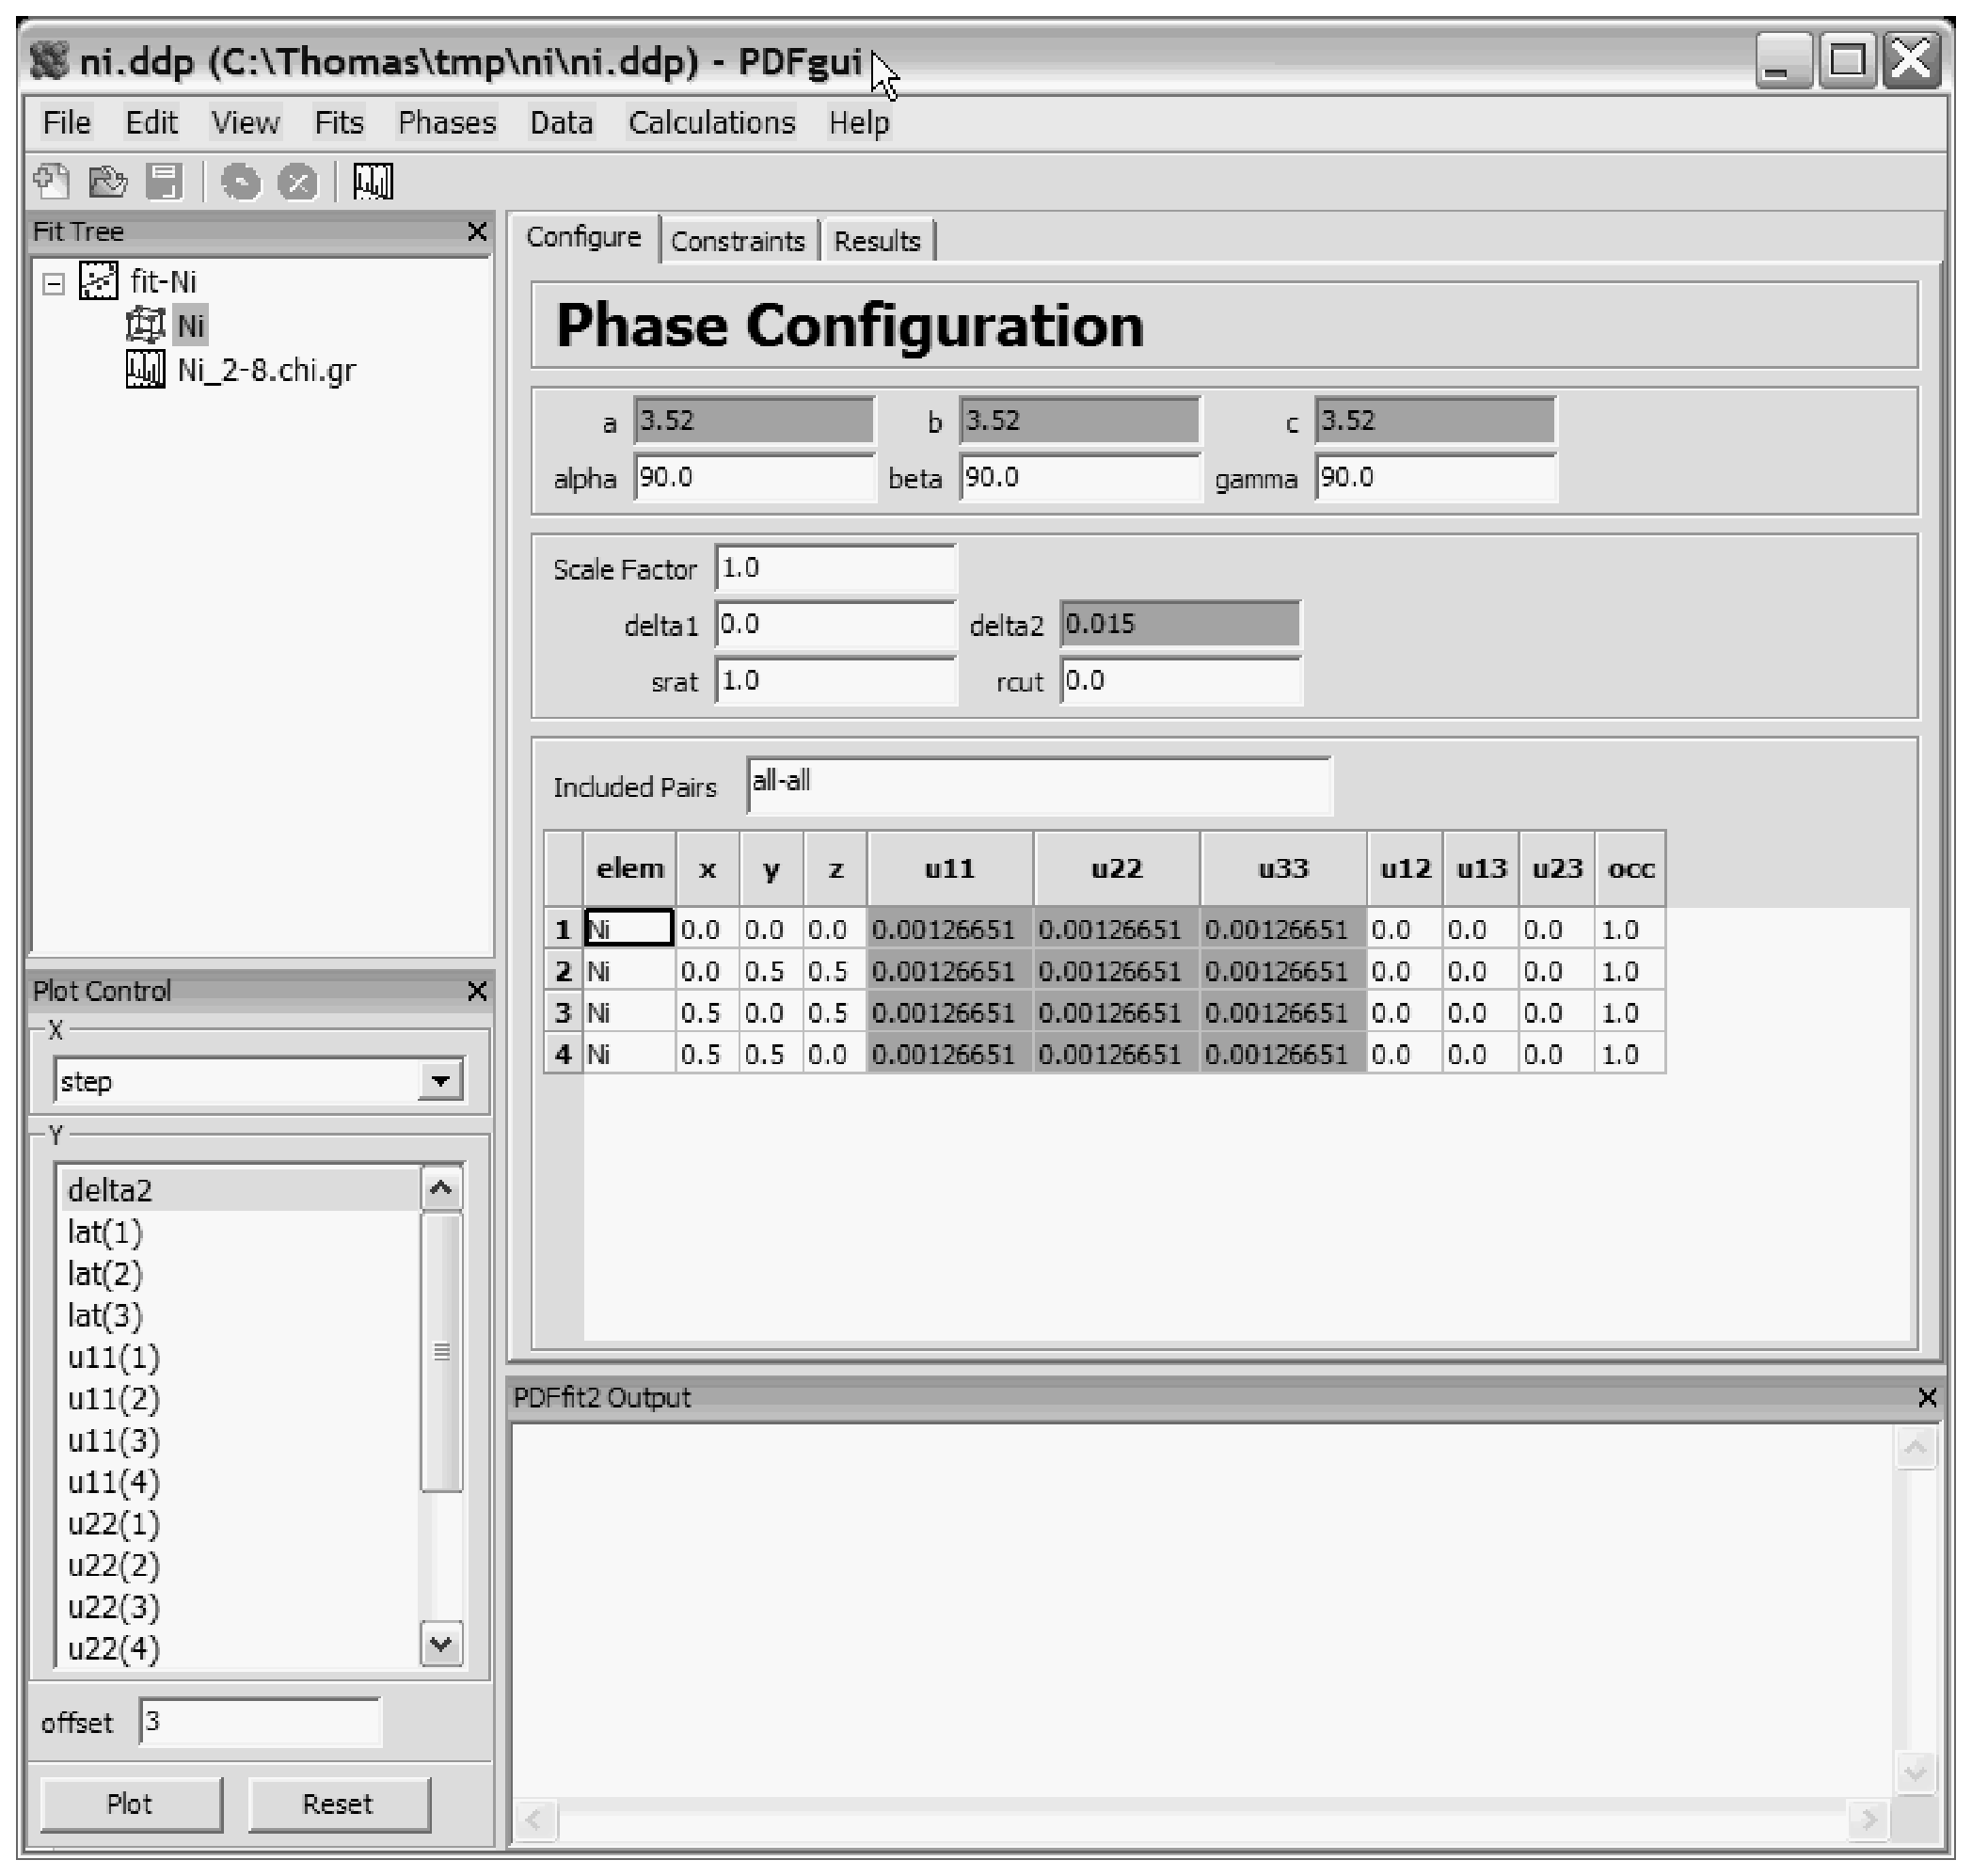
\includegraphics[width=2.5in, angle=0]{pdfnew.eps}
   \caption{Screen shot of beta version of next generation {\it PDFFIT}.}
\end{figure}


\subsection*{Version 1.3}

The main addition in this version are additional parameters to
control the PDF peak width. In addition to the quadratic term
variable, $\delta$, a linear correction has been added ($\gamma$).
In addition a PDF broadening correction determined by the instrument
resolution has been added ($\alpha$). For details on the new $r$
dependence of the PDF peak width refer to section \ref{fit_pwid}.
Following the work by \cite{thlele02}, the true PDF peak profile is
not purely a Gaussian. The corrected profile has now been
implemented in PDFFIT. Details can be found in Appendix
\ref{app-deriv}.

\subsection*{Version 1.2}

Besides various bug fixes, this new version of {\it PDFFIT} is now
distributed as self-extracting installer for the Windows operating
system. The program now supports system macros that can be
globally installed as well as reading macro files names from the
command line.

\subsection*{Version 1.1}

The following features were added to the program: {\it PDFFIT} is
now capable to export a structure in a format that can be read by
the program {\it ATOMS} \citep{prog;atoms} for 3D structural plots
(see section \ref{file_export}). The program now allows to refine
the difference between a PDF and a reference PDF. The command
language now includes simple commands for file input and output
(see section \ref{io}).

%------------------------------------------------------------------------

\section{Getting started \label{get}}

After the program {\it PDFFIT} is installed properly and the environment
variables are set, the program can be started by typing 'discus' at the
operating systems prompt. Information about the installation of {\it PDFFIT}
is given in appendix \ref{app-install}.

\begin{table}[!tbh]
\centering
\begin{tabularx}{\textwidth}{|p{30mm}|X|}
  \hline
  {\bf Symbol} & {\bf Description} \\
  \hline\hline
  "text"     &  Text given in double quotes is to be understood as typed. \\
  \hline
  $<$text$>$ &  Text given in angled brackets is to be replaced by an
                appropriate value, if the corresponding line is used
                in {\it PDFFIT}. It could, for example be the actual name
                of a file, or a numerical value. \\
  \hline
  {\tt text} &  Text in single quotes exclusively refers to {\it PDFFIT}
                commands. \\
  \hline
  $[$text$]$ &  Text in square brackets describes an optional parameter or
                command. If omitted, a default value is used, else
                the complete text given in the square brackets is to
                be typed. \\
  \hline
  \{text $|$ text\} &  Text given in curly brackets is a list of alternative
                parameters. A vertical line separates two alternative,
                mutually exclusive parameters. \\
  \hline
\end{tabularx}
\caption{\label{sym-tab}Used symbols}
\end{table}

The program uses a command language to interact with the user.  The
command {\tt exit} terminates the program and returns control to the
shell.  All commands of {\it PDFFIT} consist of a command verb,
optionally followed by one or more parameters.  All parameters must
be separated from one another by a comma ",".  There is no
predefined need for any specific sequence of commands.  {\it PDFFIT}
is case sensitive, all commands and alphabetic parameters MUST be
typed in lower case letters.  If {\it PDFFIT} has been compiled
using the {\tt -DREADLINE} option (see installation files) basic
line editing and recall of commands is possible.  For more
information refer to the reference manual or check the online help
using ('help command input').  Names of input or output files are to
be typed as they will be expected by the shell.  If necessary
include a path to the file.  All commands may be abbreviated to the
shortest unique possibility. At least a single space is needed
between the command verb and the first parameter.  No comma is to
precede the first parameter. A line can be marked as comment by
inserting a {\tt \#} as first character in the line.\par

The symbols used throughout this manual to describe commands,
command parameters, or explicit text used by the program {\it
PDFFIT} are listed in Table \ref{sym-tab}. There are several sources
of information, first {\it PDFFIT} has a build in online help, which
can be accessed by entering the command {\tt help} or if help for a
particular command $<$cmd$>$ is wanted by {\tt help $<$cmd$>$}. This
manual describes background and principle functions of {\it PDFFIT}
and should give some insight in the ways to use this program. \par

{\it PDFFIT} is distributed as part of the diffuse scattering
simulation software {\it DISCUS}.  However, {\it PDFFIT} can be used
as general plotting program separate from the {\it DISCUS} program
package.  To find out about recent updates of {\it PDFFIT} or to get
further information visit the {\it PDFFIT} WWW homepage:

\begin{center}
  {\it http://discus.sourceforge.net}
\end{center}

%------------------------------------------------------------------------

%------------------------------------------------------------------------
% Chapter:  Quickstart
%------------------------------------------------------------------------

\chapter{Quick start \label{quick}}

In order to quickly illustrated the usage of {\it PDFFIT} for those
impatient readers, a PDF refinement of $Ni$ will be illustrated. The
data used here were collected at room temperature using the diffractometer
at beamline X7A at NSLS, Brookhaven National Laboratory. The data are
terminated at $Q_{max}=22$\AA$^{-1}$. The data as well as the resulting
PDF are shown as filled circles in Figure \ref{quick-fig1}.

\begin{figure}[!b]
   \centering
   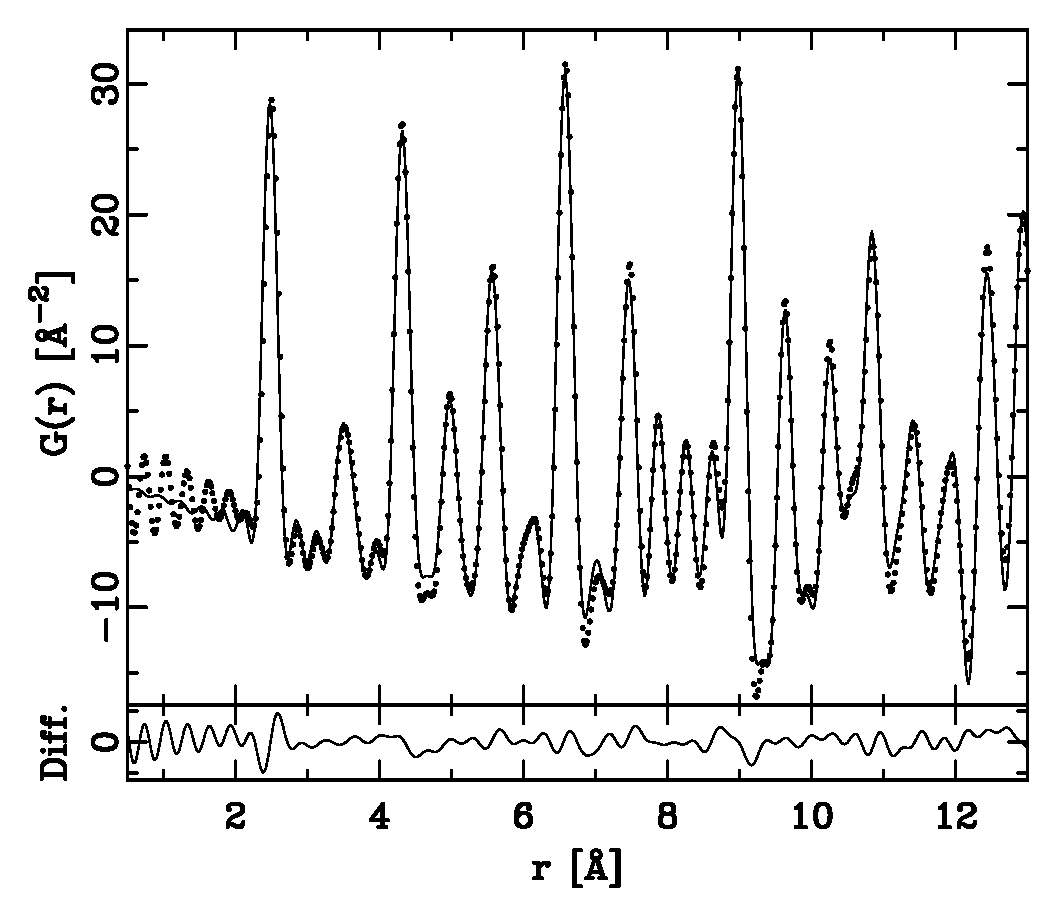
\includegraphics[scale=0.6, angle=0.0]{quick.1.eps}
   \caption[Result of PDF refinement of $Ni$]
           {Result of PDF refinement of $Ni$. The solid line is the
            calculated PDF, the filled circles are the data. A difference
            curve is plotted below the data.}
   \label{quick-fig1}
\end{figure}

The sequence of commands used to carry out the refinement is listed
below. Note that the line numbers are only added for easy reference and
are not actually part of the input. The commands can either be written
using a text editor and executed as macro file of typed in at the
{\it PDFFIT} command prompt.

\footnotesize
\begin{MacVerbatim}
      1 reset
      2 read stru,ni.stru
      3 read data,x,22.0,0.0,ni.data
      4 #
      5 par lat[1]=p[1],1.0
      6 par lat[2]=p[1],1.0
      7 par lat[3]=p[1],1.0
      8 #
      9 do i[1]=1,n[1]
     10   par u[1,i[1]]=p[2],1.0
     11   par u[2,i[1]]=p[2],1.0
     12   par u[3,i[1]]=p[2],1.0
     13 enddo
     14 #
     15 par csca[1]=p[10],1.0
     16 par qsig[1]=p[11],1.0
     17 par delt[1]=p[12],1.0
     18 #
     19 p[1]=lat[1]
     20 p[2]=u[1,1]
     21 #
     22 p[10]=1.50
     23 p[11]=0.03
     24 p[12]=0.10
     25 #
     26 range 1,0.5,13.0
     27 run
     28 #
     29 save pdf,1,ni_ref.calc
     30 save dif,1,ni_ref.dif
     31 save stru,1,ni_ref.stru
     32 save res,ni_ref.out
\end{MacVerbatim}
\normalsize

\noindent The command {\tt reset} in line 1 resets {\it PDFFIT} to
have a defined initial state. Next a structural model (line 2) and
the experimental PDF (line 3) are read. The format of these text
files are discussed in section \ref{file} of this manual. The
parameters of the command {\tt read data} are the radiation type
(here X-ray), $Q_{max}$ and the resolution factor $\sigma_{Q}$
associated with the data file '{\it ni.data}'. {\it PDFFIT} allows
the user to freely define relations between structural and
experimental parameters and the refinement parameters {\tt p[i]}.
This is done using the command {\tt par}. The lattice parameters
$a,b,c$ are stored in {\it PDFFIT} variables {\tt lat[1], lat[2]}
and {\tt lat[3]}. In lines 5--7 of the example above refinement
parameters {\tt p[1]} is used to refine all three lattice
parameters since $Ni$ is cubic and $a=b=c$. The additional
parameter {\tt 1.0} is the derivative of the parameter on the left
with respect to the refinement parameters. These derivatives are
needed for the least-squares refinement (see Appendix
\ref{app-deriv} for details). In our case we have a simple one to
one correspondence and the derivative is trivial. In lines 9--13
the temperature factors $U_{lm}$ of the atoms are associated with
a single refinement parameter {\tt p[2]}. Note that we have four
$Ni$ sites in our model and rather than typing the definitions for
each atom separately, we are using a loop. Details about loops and
variables are given in section \ref{fort}, all we need to know for
now is that the variable {\tt n[1]} contains the number of sites.
In our example we only refine an isotropic temperature factor, so
we use the same parameter for $U_{11}, U_{22}$ and $U_{33}$ stored
in {\tt u[1,n], u[2,n]} and {\tt u[3,n]}. Next we associate
individual refinement parameters with the scale factor $f_{p}$
(line 15), the resolution factor $\sigma_{Q}$ (line 16) and the
dynamic correlation factor $\delta$ (line 17). Note that there is
no need for a consecutive numbering of the parameters. Finally we
need to initialize the refinement parameters {\tt p[i]} with
suitable starting values which is done in lines 19--24. Last we
define the $r$-range we want to use for the refinement (line 26),
here from 0.5\AA\ to 13.0\AA. The argument of the {\tt range}
command is the number of the dataset (see section \ref{fit_mult}).
There is generally no predefined order for the commands, however,
data need to be read first and obviously all desired settings must
be entered before the refinement is started using the command {\tt
run} (line 27). The screen output during the refinement is shown
below:

\footnotesize
\begin{MacVerbatim}
     Starting refinement ...
     --------------------------------------------------------------------------
     Iteration  :   0  Sum:  48995.5     Urf:  1.00798
                       R  : 0.155190     Rw : 0.154659
     Parameters :
       1:  3.52032       2: 0.515471E-02  10:  1.50000      11: 0.300000E-01
      12: 0.100000
     --------------------------------------------------------------------------
     Iteration  :   1  Sum:  44646.7     Urf:  1.00165
                       R  : 0.148137     Rw : 0.147636     DRw: -.702314E-02
     Parameters :
       1:  3.51974       2: 0.505564E-02  10:  1.48549      11: 0.313635E-01
      12: 0.127834
     --------------------------------------------------------------------------
     Iteration  :   2  Sum:  44352.0     Urf:  1.00089
                       R  : 0.147658     Rw : 0.147148     DRw: -.488088E-03
     Parameters :
       1:  3.52014       2: 0.501998E-02  10:  1.48752      11: 0.319241E-01
      12: 0.131231
     --------------------------------------------------------------------------
     Iteration  :   3  Sum:  49266.2     Urf:  1.00054
                       R  : 0.155582     Rw : 0.155086     DRw: 0.793780E-02
     Parameters :
       1:  3.52056       2: 0.501416E-02  10:  1.48125      11: 0.286770E-01
      12: 0.135971
     --------------------------------------------------------------------------
\end{MacVerbatim}
\normalsize

\noindent For each iteration the program prints $\sum
(G_{obs}-G_{calc})^{2}$ ({\tt sum}), the R-value ({\tt R}), the
weighted R-value ({\tt Rw}) and the difference of the R-value
compared to the previous cycle ({\tt DRw}). Furthermore the actual
values of all refinement parameters {\tt p[i]} are listed. Note
that iteration 3 has a slightly higher R-value compared to
iteration 2, so the refinement converged or exploded depending on
the size of the (now positive) difference. The resulting
parameters correspond actually to the output of the $(n-1)$th
cycle. However, the display of the iteration that lead to the
termination of the refinement might help to judge how well the fit
converged. \par

In lines 29--32 we have to save the resulting PDF, the difference between
observed and calculated PDF, the resulting structure and
fit results, respectively. The calculated PDF can be plotted using
e.g. {\it KUPLOT} which is part of the {\it DISCUS} software package.
Figure \ref{quick-fig1} was generated using {\it KUPLOT}. The final
structure can also be exported in {\it DISCUS} format for further
analysis. \par

After this quick run through a quite simple example refinement we will
discuss all features of the program {\it PDFFIT} in more detail.
Additionally the command reference and the online help of the program
might be a valuable source of information. Use the command {\tt help}
when in {\it PDFFIT} to activate the online help facility of the
program.

%------------------------------------------------------------------------

%------------------------------------------------------------------------
% Chapter:  File formats
%------------------------------------------------------------------------

\chapter{File formats \label{file}}
\section{PDF data files \label{file_pdf}}

The file format for observed as well as calculated PDFs used by
{\it PDFFIT} are simple text files of the following general format
per data point:

\begin{quote}
  {\it r $\cdot$ G(r) $\cdot$  $\sigma(r)$ $\cdot$ $\sigma(G(r))$}
\end{quote}

Each data point is on a separate line in the file. The first column
contains the value of $r$ given in units of \AA. The second column
is $G(r) = 4 \pi r [\rho(r) - \rho_{0}]$ in units of \AA$^{-2}$. The
third column is ignored by {\it PDFFIT} but is required to be
compatible with the plot program {\it KUPLOT} where it takes the
value of the standard deviation of $r$. The last column contains the
standard deviation of $G(r)$ which is used to calculate the weight
$w(r)$ according to $w(r) = 1/\sigma^{2}(G(r))$. A short listing of
a PDF file is shown below:

\begin{MacVerbatim}
     0.020000    11.687810      0.0       0.081738
     0.040000    22.659353      0.0       0.155914
     0.060000    31.915903      0.0       0.212270
        :
    19.960000   -14.941482      0.0       0.162837
    19.980000   -14.858703      0.0       0.163509
    20.000000   -14.135623      0.0       0.164080
\end{MacVerbatim}

As one can see, column 3 is just occupied by some dummy number.
However, the current version of {\it PDFFIT} will also read
two-column files ($r G(r)$) and three-column files ($r G(r) w(r)$).
In order to save disk space, archived files might be compressed
using e.g. {\tt gzip}. The results can be plotted using {\it KUPLOT}
or any other visualization software that can import ASCII files.

%------------------------------------------------------------------------

\section{Structure files \label{file_stru}}

The program {\it PDFFIT} uses a keyword driven structure file format
similar to the one used by {\it DISCUS}. However, the philosophy of
{\it DISCUS} is based on simulating large disordered structures. Thus
{\it DISCUS} does not support site occupancies and includes only an
isotropic temperature factor. Furthermore, {\it PDFFIT} calculates
standard deviations for its structural parameters which need to be
saved as well. We will have a look at the $Ni$ structure files used
in the last section. The {\it DISCUS} version of this file looks like
this:

\begin{MacVerbatim}
    title Ni
    spcgr P1
    cell  3.520323,    3.520323,    3.520323,   90.0,   90.0,   90.0
    ncell 1,1,1, 4
    atoms
    NI      .000000   .000000   .000000     0.4070
    NI      .000000   .500000   .500000     0.4070
    NI      .500000   .000000   .500000     0.4070
    NI      .500000   .500000   .000000     0.4070
\end{MacVerbatim}

The file contains a title, the space group and lattice parameters in
the first three lines. The lattice parameters are again given in
units of \AA. Some explanation needs to be given concerning the
space group. The program {\it PDFFIT} ignores the space group and
just stores it to write it back in the output file. Thus no
symmetrically equivalent atom positions are created using the space
group symbol and there are no symmetry restrictions during the
refinement unless coded in the refinement parameter definitions. A
convenient way to handle systems with many symmetrically equivalent
positions is to create a similar file with the correct space group
symbol and read it with {\it DISCUS} as a {\tt cell} file. This will
generate all required positions and when saving it as a {\tt stru}
file, all positions are saved and can be read by {\it PDFFIT}. The
{\tt ncell} keyword in the input file above specifies the number of
unit cells in $x,y$ and $z$-direction and the number of atoms within
one unit cell. This way it is possible to construct a model using a
supercell based on several basic unit cells without having to change
the metric. The last keyword needs to be {\tt atoms} followed by a
list of atoms. Each line contains the atom name, the position in
fractional coordinates and the isotropic temperature factor B (see
below). When using more than one unit cell, the fractional
coordinates range from $-N/2$ to $N/2$ for $N$ unit cells. The atom
list must follow a specific order outlined in the {\it DISCUS}
manual. \par

\begin{MacVerbatim}
    title  Ni
    format pdffit
    scale  1.4875
    spcgr  P1
    cell   3.520144,  3.520144,  3.520144, 90.000000, 90.000000, 90.000000
    dcell  0.000031,  0.000031,  0.000031,  0.000000,  0.000000,  0.000000
    ncell  1,1,1, 4
    atoms
    NI      0.00000000        0.00000000        0.00000000       1.0000
            0.00000000        0.00000000        0.00000000       0.0000
            0.00501998        0.00501998        0.00501998
            0.00000515        0.00000515        0.00000515
            0.00000000        0.00000000        0.00000000
            0.00000000        0.00000000        0.00000000
\end{MacVerbatim}

This is the corresponding file in {\it PDFFIT} format. Only one $Ni$
atom is shown for brevity. We note three new keywords, {\tt format}
specifies that this is a {\it PDFFIT} file which can not be read by
{\it DISCUS}. The keyword {\tt scale} gives the scale factor used
for the structural phase defined in this file and {\tt dcell}
defines the standard deviations of the lattice parameters which
might be needed to calculate bond-length and angles with propagated
errors. For each atom, the following information is given: atom
name, position $x,y,z$, occupancy $o$, standard deviations
$\sigma(x), \sigma(y), \sigma(z)$ and $\sigma(o)$ followed by the
three diagonal elements of the anisotropic temperature factor
$U_{11}, U_{22}, U_{33}$ with errors and the three elements $U_{12},
U_{13}, U_{23}$ with errors. {\it PDFFIT} recognises both types of
structure file automatically and converts the $B$ value to $U_{ii}$
according to $U_{11} = U_{22} = U_{33} =
 / 8 \pi^{2}$ and $U_{12} = U_{13} = U_{23} = 0$ \citep{sands}.
\par

When saving structure files one can choose between {\it PDFFIT}
format ({\tt save pdf,..}) and {\it DISCUS} format ({\tt save
disc,..}). When using the {\it DISCUS} format, information about
site occupancies and errors are lost and the $B$ value is
calculated as $B = 8 \pi^{2} [U_{11} + U_{22} + U_{33}]/3$.
Obviously any anisotropy is lost. However, {\it DISCUS} can be
used to export the structure for plotting, doing further analysis
or calculating single crystal diffuse scattering from the refined
model. We will give a short example of how to use {\it DISCUS} to
expand the content of unit cell using the space group symbol. The
input file for {\it DISCUS} for $GaAs$ would look like this:

\begin{MacVerbatim}
    title GaAs
    spcgr F-43m
    cell 5.6537  5.6537  5.6537  90.0  90.0  90.0
    atoms
    GA    0.0000  0.0000  0.0000  1.0000
    AS    0.2500  0.2500  0.2500  1.0000
\end{MacVerbatim}

The following sequence of {\it DISCUS} commands can be used to read
the unit cell file, expand it to a structure of 1x1x1 unit cells and
save the result to the file '{\it gaas.stru'}:

\begin{MacVerbatim}
    read
    cell gaas.cll,1,1,1
    save gaas.stru
\end{MacVerbatim}

\begin{figure}[!t]
   \centering
   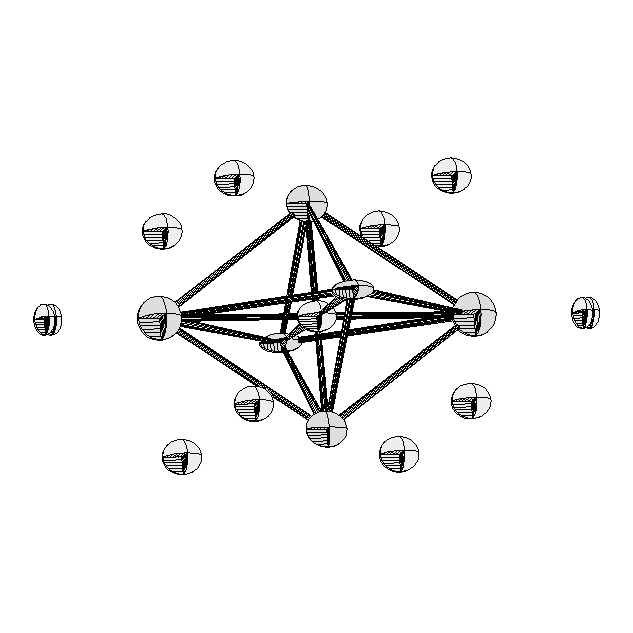
\includegraphics[scale=0.65, angle=0]{fil.1.eps}
   \caption[ATOMS structure plot example]
           {ATOMS structure plot displaying thermal ellipsoids.}
   \label{fil_fig1}
\end{figure}

The structure file saved by {\it DISCUS} contains all atom positions
generated by the space group $Fm\overline{3}m$. The output file
containing the expected eight atoms is listed below:

\begin{MacVerbatim}
    title GaAs
    spcgr F-43m
    cell    5.6537    5.6537    5.6537   90.0   90.0   90.0
    ncell   1,1,1, 8
    atoms
    GA     0.0000    0.0000    0.0000      1.000
    GA     0.0000    0.5000    0.5000      1.000
    GA     0.5000    0.0000    0.5000      1.000
    GA     0.5000    0.5000    0.0000      1.000
    AS     0.2500    0.2500    0.2500      1.000
    AS     0.2500    0.7500    0.7500      1.000
    AS     0.7500    0.2500    0.7500      1.000
    AS     0.7500    0.7500    0.2500      1.000
\end{MacVerbatim}

Note that this version of the file contains the {\tt ncell} keyword.
This example was quite simple since all the atoms are on special
positions and only the F-centering is applied. However, when dealing
with atoms on general positions in a high symmetry space group using
{\it DISCUS} to generate all symmetrically equivalent positions is a
real time saver.

%------------------------------------------------------------------------

\section{Exporting structures \label{file_export}}

{\it PDFFIT} can also export the structure in a format using the
command {\tt save atoms,1,file} (assuming phase number 1 to be
saved). This file can be imported by the structure plotting program
{\it ATOMS} \citep{prog;atoms} using the menu {\it File
$\rightarrow$ Import File $\rightarrow$ Free-Form (.INP)}. An
example displaying thermal ellipsoids can be seen in Figure
\ref{fil_fig1}. The bonds were added in {\it ATOMS}. In order for
{\it ATOMS} to display the complete exported structure, the lattice
parameters and fractional coordinates are adjusted so that the
complete crystal is a single unit cell. Additionally the space group
is set to be $P1$.

%------------------------------------------------------------------------

%------------------------------------------------------------------------
% Chapter:  Calculation the PDF
%------------------------------------------------------------------------

\chapter{PDF calculation \label{calc}}
\section{Simple PDF calculation \label{calc_pdf}}

Sometimes rather than refining a PDF one simply wants to calculate
one from a structural model e.g. to explore the effect of a certain
parameter on the calculated PDF. Rather than starting a refinement
with no refinement parameters {\it PDFFIT} offers the simple command
{\tt calc} to compute the desired PDFs. As an example we want to
calculate the PDF of $Ni$ with two different termination values
$Q_{max}$. The corresponding sequence of {\it PDFFIT} commands is
shown below.

\footnotesize
\begin{MacVerbatim}
      1 reset
      2 read stru,ni.stru
      3 alloc n,25.0,0.0,1.5,6.5,251
      4 delt[1]=0.3
      5 #
      6 calc
      7 save pdf,1,cal_25.calc
      8 #
      9 qmax[1]=35.0
     10 calc
     11 save pdf,1,cal_35.calc
\end{MacVerbatim}
\normalsize

\noindent The first two command should be familiar already from
the example in section \ref{quick}. In line 3 we allocate the
required space for the PDF we want to calculate without actually
reading any experimental data. The first three parameters of the
{\tt alloc} command are similar to {\it read data} in the earlier
example, they specify the radiation type and values for $Q_{max}$
and the resolution factor $\sigma_{Q}$. The next two values
specify the desired $r$-range which in our example is $1.5$ to
$6.5$\AA. The last parameter is the number of data points we want
which in our example leads to a grid size of $\Delta r =
(6.5-1.5)/(251-1) = 0.02$\AA. In order to see a larger effect, we
set the dynamic correlation factor $\delta$ to a rather large
value in line 4 which gives us quite a sharp first PDF peak. Now
the PDF can be calculated using the command {\tt calc} (line 6)
and the result is saved to the file '{\it cal\_25.calc}' (line 7).
In order to recalculate the same PDF with a different value of
$Q_{max}$, we simply alter the value using the corresponding
variable {\tt qmax[1]} (line 9). Note that the '1' specifies the
number of the data set. Finally we calculate the PDF again (line
10) and save the result to a different file (line 11).

\begin{figure}[!htb]
   \centering
   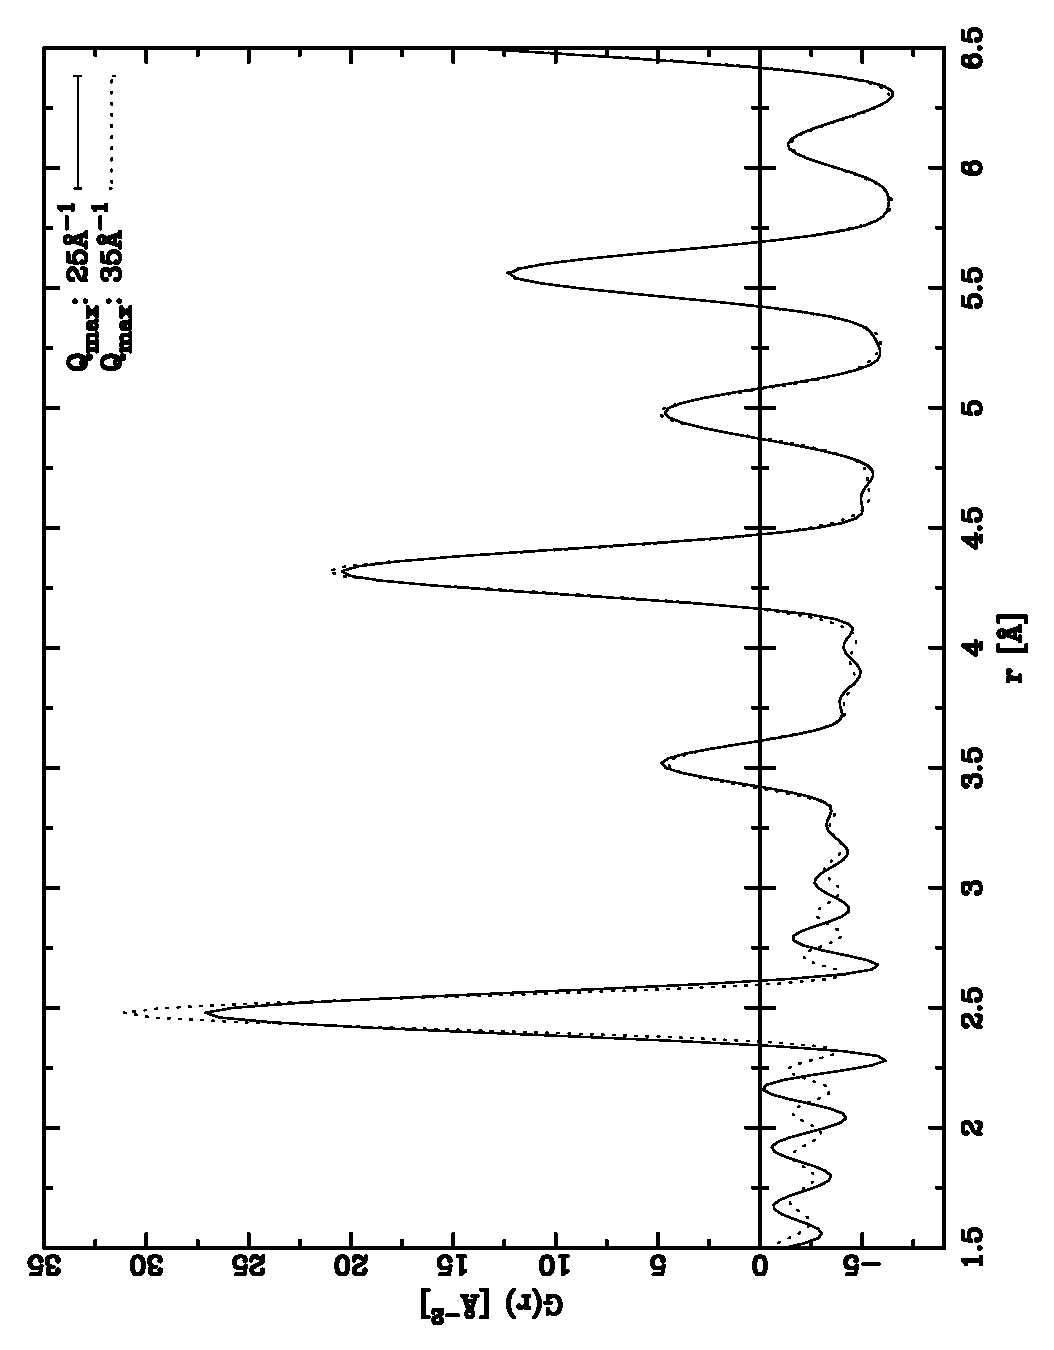
\includegraphics[scale=0.5, angle=270]{cal.1.eps}
   \caption[Calculated PDFs for $Ni$ at different values $Q_{max}$]
           {Calculated PDFs for $Ni$ at different values $Q_{max}$.
            The solid line is the PDF with $Q_{max} = 25$\AA$^{-1}$ and
            the dotted line is for $Q_{max} = 35$\AA$^{-1}$.}
   \label{cal-fig1}
\end{figure}

The result of the example given above is shown in Figure \ref{cal-fig1}.
As one might expect, the termination ripples for the calculation with
the higher $Q_{max}$ show a higher frequency. In addition we can observe
in our particular example that the intrinsic width of the first peak
is smaller than the width of the convolution at $Q_{max}=25$\AA$^{-1}$,
in other words the peak is broadened due to the $Q$ termination.

%------------------------------------------------------------------------
\section{Calculating partial or differential PDFs \label{calc_partial}}

When discussing equation (\ref{eq_igr}) used to calculate the PDF from
a structural model, we just stated that the sum over $ij$ goes over
{\it all} pairs of atoms $i$ and $j$ within the model crystal. This
is perfectly correct to calculate a total PDF. However sometimes it
might be desired to calculate just a partial or differential PDF. Let
us consider $GaAs$ as a simple example. Figure \ref{cal-fig2} shows
the total PDF as well as the differential and partial $Ga$ PDF of
$GaAs$. The total PDF is shown in the top view graph of Figure
\ref{cal-fig2}. Numbering the PDF peaks from the left, we find that
the first peak corresponds to the shortest $Ga-As$ distance. The second
peak is from $Ga-Ga$ and $As-As$ separated by the F-centering, the
next peak is again from $Ga-As$, the fourth peak corresponds to the
lattice repeat and so on. Let us consider just the first two peaks.
A differential PDF contains all pairs of one specific atom, here $Ga$,
and all other atoms. So the first $Ga-As$ peak is the same in the
differential PDF (Fig. \ref{cal-fig2} middle) as in the total one.
The second peak, however, contains contributions of $Ga-Ga$ and
$As-As$ in the total PDF, whereas the differential PDF shows no
$As-As$ pairs. Since there is the same number of both types, the second
peak in the differential PDF has only half the height compared to
the total PDF. The partial $Ga$ PDF (Fig. \ref{cal-fig2} bottom) contains
only contributions of $Ga-Ga$ pairs. Thus the first peak is missing
whereas the second peak is equivalent to the one observed in the
differential PDF. \par

\begin{figure}[!htb]
   \centering
   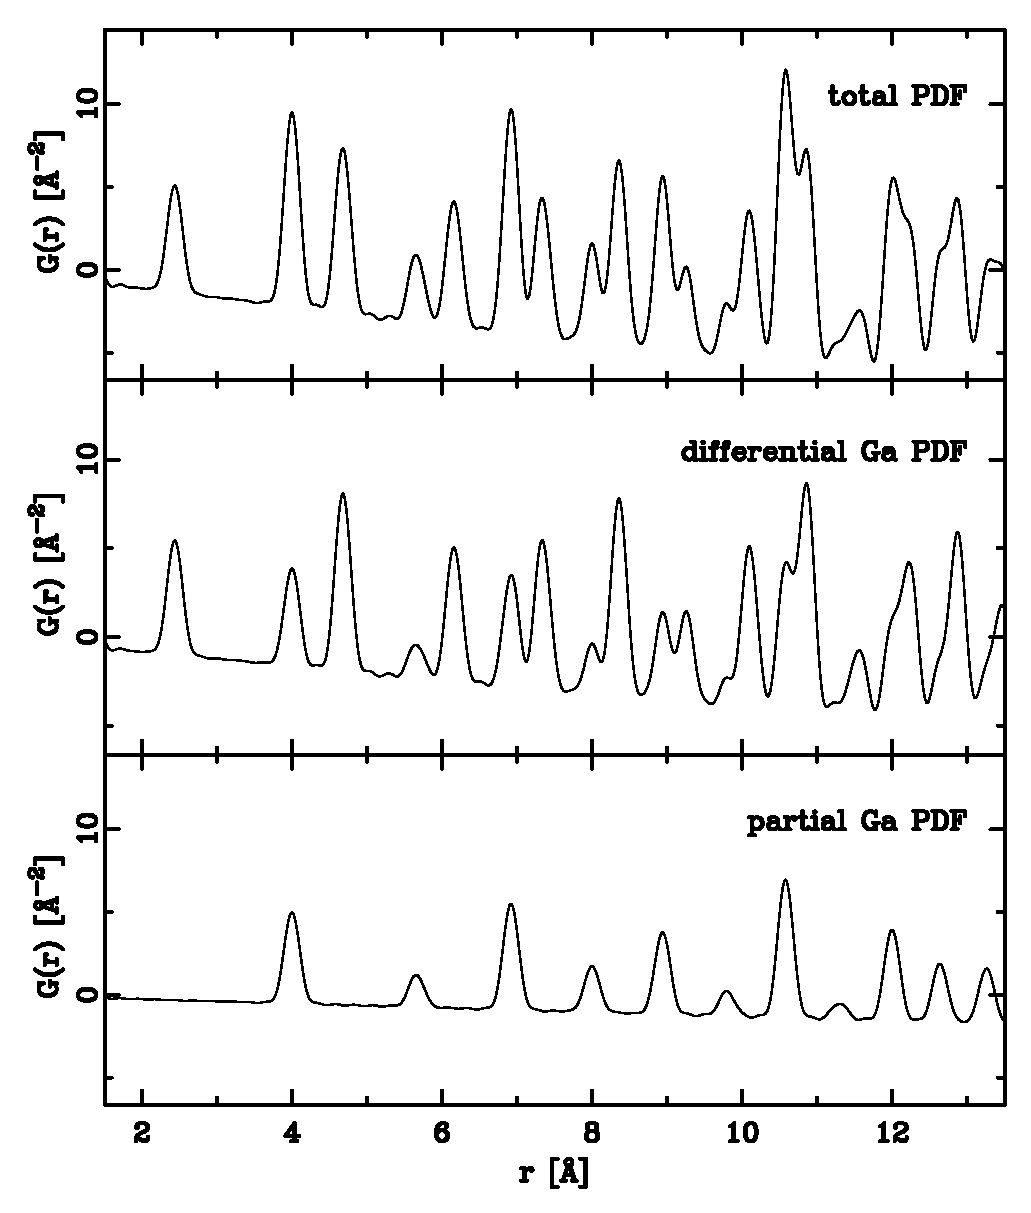
\includegraphics[scale=0.6, angle=0]{cal.2.eps}
   \caption[Total, differential and partial PDF of $GaAs$]
           {Top: Total $GaAs$ PDF. Middle: Differential $Ga$ PDF of
            $GaAs$. Bottom: Partial $Ga$ PDF of $GaAs$.}
   \label{cal-fig2}
\end{figure}

The determination which atoms contribute to which peaks in the PDF
is not always as simple as in our $GaAs$ example and the calculation
of various partial PDFs might help to understand a more complex
PDF. \par

The macro that was used to calculate the PDFs shown in Figure \ref{cal-fig2}
is listed below. Again the line number were added for convenience. The
first three lines are similar to the example in the last section. The
commands to select particular atom types are {\tt isel} and {\tt jsel}.

\footnotesize
\begin{MacVerbatim}
      1 reset
      2 read stru,gaas.stru
      3 alloc x,25.0,0.0,1.5,13.5,601
      4 #
      5 isel 1,all
      6 jsel 1,all
      7 calc
      8 save pdf,1,tot.calc
      9 #
     10 ides 1,all
     11 jdes 1,all
     12 isel 1,ga
     13 jsel 1,all
     14 calc
     15 save pdf,1,dif_ga.calc
     16 #
     17 ides 1,all
     18 jdes 1,all
     19 isel 1,ga
     20 jsel 1,ga
     21 calc
     22 save pdf,1,par_ga.calc
\end{MacVerbatim}
\normalsize

\noindent To calculate the total PDF, we simply select all atom
types present in the structure (lines 5--6) and calculate and save
the PDF (lines 7--8). Note that the selection of all atoms is the
default when starting {\it PDFFIT} or using the command {\tt
reset}. The first parameter of the {\tt i/jsel} and {\tt i/jdes}
commands is the corresponding data set number, here simply one. To
calculate the differential PDF we select $Ga$ for atom $i$ (line
12) and all atoms for atom $j$ (line 13). Since the command {\tt
isel} or {\tt jsel} adds the specified atom to the list of allowed
atoms, we need to deselect all previously selected atoms first as
done in lines 10--11 of our example. Again we calculate and save
the new PDF (lines 14--15). Finally we select just $Ga$ for atoms
$i$ and $j$ (lines 17--20) to obtain the partial $Ga$ PDF and
recalculate and save the result (lines 21-22). \par

Note, that {\it PDFFIT} can also refine a experimental differential PDF
which for example can be obtained from anomalous X-ray scattering. The
required commands to select the specific atom types are exactly the same
as in this example. Note, that {\it PDFFIT} normalizes the number density
$\rho_{0}$ by a weighting factor given below:

\begin{equation}
  w(kl) = \frac{\sum_{kl} c_{k}c_{l}b_{k}b_{l}}
               {\sum_{ij} c_{i}c_{j}b_{i}b_{j}}
  \label{eq_norm}
\end{equation}

Here the sum over $kl$ is only over those atom that are selected
and contribute to the PDF whereas $ij$ sums over all atoms within the
crystal. It is immediately obvious that $w(kl)=1.0$ for the total
PDF. This definition is consistent with the use of Faber-Ziman
partial structure factors. For details refer to \cite{waseda} and
appendix \ref{app-deriv}.

%------------------------------------------------------------------------

%------------------------------------------------------------------------
% Chapter:  FORTRAN interpreter
%------------------------------------------------------------------------

\chapter{FORTRAN style interpreter \label{fort}}

The program includes a FORTRAN style interpreter that allows the
user to program complex modifications.  The interpreter provides
variables, linked to data sets and free variables, loops, logical
construction, basic arithmetic and built in functions.  Commands
related to the FORTRAN interpreter are {\tt =, break, do, else,
elseif, enddo, endif, eval, if} and {\tt variable}. The command {\tt
eval} allows to examine the contents of a variable of evaluate an
expression, e.g. {\tt eval r[1]*0.5}. \par

%------------------------------------------------------------------------

\section{Variables \label{var}}

There are two types of variables: user defined single named
variables of type integer or real and build in variables, denoted by
a name, immediately followed by a left square bracket [, one or more
indices and a right square bracket ]. An example of the use of
defined variables is shown here:
%
\begin{MacVerbatim}
   1  variable  real,alpha,90.0
   2  variable  real,beta
   3  variable  real,diff
   4  beta = 94.0
   5  diff = alpha - beta
   6  eval diff
\end{MacVerbatim}
%
In line one we define a real variable {\tt alpha} with an initial
value of 90. Next two more variables are defined and the difference
between {\tt alpha} and {\tt beta} is calculated (line 5) and the
result displayed on the screen (line 6). Examples for build in
variables are given next.

\begin{quote}
  {\it Example :\/} i[1], r[0], i[i[1]], x[1,2]
\end{quote}

The left square brackets {\bf must} immediately follow the name of
the variable.  Blanks within the square brackets are not
significant.  The index can be any integer expression, especially
any of the integer variables again.  Two free variables are
provided, an integer, {\tt i[n]}, and a real, {\tt r[n]} variable.
Each of these variables is actually an array of dimension n given in
squared brackets. The allowed range for n is 0 to MAXPARAM, which is
defined at compilation time by the parameter MAXPARAM in the file
{\it param.inc}. More details are given in appendix
\ref{app-install}. \par

Beside these variables {\tt i[n]} and {\tt r[n]} for general use a
large variety of variables is linked to specific information of {\it
PDFFIT}, e.g. of the currently loaded structural data or PDF data.
Some of these variables c an not be modified, others like atomic
positions or thermal factors can be altered, thus allowing to modify
the loaded structure. Table \ref{v1-tab} shows a summary of {\it
PDFFIT} specific variables related to a loaded structure. Note that
all structure related variables are linked to the currently active
phase. To alter structural information of another phase use the
command {\tt phase} first. Variables related to PDF data are listed
in Table \ref{v2-tab} and refinement variables can be found in Table
\ref{v3-tab}.

\begin{table}[!htb]
\centering
\begin{tabularx}{\textwidth}{|p{30mm}|X|}
  \hline
  {\bf Variable} & {\bf Description} \\
  \hline \hline
  {\tt n[1]}$^{*}$ & Total number of atoms of current phase \\
  {\tt n[2]}$^{*}$ & Number of different atoms of current phase \\
  {\tt n[3]}$^{*}$ & Number of atoms per unit cell (current phase) \\
  {\tt n[4]}$^{*}$ & Number of phases \\
  {\tt n[5]}$^{*}$ & Number of currently active phase \\
  \hline
  {\tt x[n]}      & x-position of atom n of current phase \\
  {\tt y[n]}      & y-position of atom n of current phase \\
  {\tt z[n]}      & z-position of atom n of current phase \\
  {\tt m[n]}      & Number of atom type on site n (current phase) \\
  {\tt u[i,n]}    & Anisotropic thermal factor $U_{lm}$ for site n with
                    ($i=1..6$ for $U_{11}, U_{22}, U_{33}, U_{12}, U_{13},
                     U_{23}$)\\
  {\tt o[n]}      & Occupancy of site n (current phase) \\

  {\tt lat[i]}    & Lattice parameters ($i=1..6$ for $a,b,c,\alpha,\beta,
                    \gamma$) \\
  {\tt csca[p]}   & Scaling factor $f_{p}$ for phase $p$ \\
  {\tt rhoz[p]}   & Number density $\rho_{0}$ for phase $p$ \\
  \hline
\end{tabularx}
\caption[{\it PDFFIT} structural variables]
        {\label{v1-tab}{\it PDFFIT} structural variables. Variables marked
         with $^{*}$ are read-only and can not be altered.}
\end{table}

\begin{table}[!htb]
\centering
\begin{tabularx}{\textwidth}{|p{30mm}|X|}
  \hline
  {\bf Variable} & {\bf Description} \\
  \hline \hline
  {\tt n[6]}$^{*}$    & Number of loaded experimental PDFs \\
  {\tt np[s]}$^{*}$   & Number of data points of data set $s$ \\
  \hline
  {\tt pc[n,s]}       & Value of calculated PDF point $n$ of data set
                        $s$ for current phase \\
  {\tt po[n,s]}       & Value of observed PDF point $n$ of data set $s$ \\
  {\tt pw[n,s]}       & Value of weight ($1/\sigma^{2}$) of point $n$
                        of data set $s$ \\
  \hline
  {\tt rmin[s]}       & Minimum $r$-value for dataset $s$ \\
  {\tt rmax[s]}       & Maximum $r$-value for dataset $s$ \\
  {\tt delr[s]}       & Step size $\Delta r$ for dataset $s$ \\
  {\tt rang[i,s]}     & Range in $r$ to be calculated or refined ($i=1,2$
                        for lower and upper limit) \\
  \hline
  {\tt delt[p]}       & Value of $\delta$ for quadratic PDF peak sharpening for
                        phase $p$\\
  {\tt gamm[p]}       & Value of $\gamma$ for linear PDF peak sharpening for
                        phase $p$\\
  {\tt rcut[p]}       & Value of $r_{cut}$ below which the PDF peak width
                        is multiplied with $\phi_{0}$ \\
  {\tt srat[p]}       & Value of $\phi_{0}$ (or $\sigma$-ratio) \\
  {\tt qmax[s]}       & Maximum $Q$-value for data set $s$ \\
  {\tt qalp[s]}       & Value of $\alpha(s)$ (resolution broadening) for
                        data set $s$ \\
  {\tt qsig[s]}       & Value of $\sigma_{Q}$ (resolution dampening) for
                        data set $s$ \\
  {\tt dsca[s]}       & Scale factor $f_{s}$ for data set $s$ \\
  {\tt bave[s]}       & Average scattering length \\
  \hline
\end{tabularx}
\caption[{\it PDFFIT} PDF related variables]
        {\label{v2-tab}{\it PDFFIT} PDF related variables. Variables marked
         with $^{*}$ are read-only and can not be altered.}
\end{table}

\begin{table}[!htb]
\centering
\begin{tabularx}{\textwidth}{|p{30mm}|X|}
  \hline
  {\bf Variable} & {\bf Description} \\
  \hline \hline
  {\tt n[7]}$^{*}$    & Maximum number of parameters \\
  {\tt n[8]}$^{*}$    & Number of used refinement parameters \\
  \hline
  {\tt p[n]}          & Value of refinement parameter $p_{n}$ \\
  {\tt dp[n]}$^{*}$   & Standard deviation of {\tt p[n]} \\
  {\tt pf[n]}         & Refinement flag for $p_{n}$ (1=refine, 0=fixed) \\
  {\tt cl[n,m]}$^{*}$ & Value of correlation between parameters $p_{n}$ and
                        $p_{m}$ \\
  {\tt rw[1]}$^{*}$   & Expected R-value of refinement \\
  {\tt rw[2]}$^{*}$   & Resulting R-value of refinement \\
  {\tt rw[3]}$^{*}$   & Resulting weighted R-value of refinement \\
  \hline
  {\tt dx[n]}          & Standard deviation of {\tt x[n]} \\
  {\tt dy[n]}          & Standard deviation of {\tt y[n]} \\
  {\tt dz[n]}          & Standard deviation of {\tt z[n]} \\
  {\tt du[i,n]}$^{*}$  & Standard deviation of {\tt u[i,n]} \\
  {\tt do[n]}$^{*}$    & Standard deviation of {\tt o[n]} \\
  {\tt drhoz[p]}$^{*}$ & Standard deviation of {\tt rhoz[p]} \\
  {\tt dlat[i]}        & Standard deviation of {\tt lat[i]} \\
  {\tt ddelt[n]}$^{*}$ & Standard deviation of {\tt delt[n]} \\
  {\tt dgamm[n]}$^{*}$ & Standard deviation of {\tt gamm[n]} \\
  {\tt dsrat[n]}$^{*}$ & Standard deviation of {\tt srat[n]} \\
  {\tt dcsca[n]}$^{*}$ & Standard deviation of {\tt csca[n]} \\
  {\tt ddsca[s]}$^{*}$ & Standard deviation of {\tt dsca[s]} \\
  {\tt dqsig[s]}$^{*}$ & Standard deviation of {\tt qsig[s]} \\
  {\tt dqalp[s]}$^{*}$ & Standard deviation of {\tt qalp[s]} \\
  \hline
\end{tabularx}
\caption[{\it PDFFIT} refinement variables]
        {\label{v3-tab}{\it PDFFIT} refinement variables. Variables marked
         with $^{*}$ are read-only and can not be altered.}
\end{table}

Another variable is {\tt res[i]} which contains the results of a
particular {\it PDFFIT} command. The variable {\tt res[0]} contains
the number of elements returned in {\tt res[i]}. Check the online
help for the different commands to see what results might be
returned in this variable. \par

%------------------------------------------------------------------------

\section{Arithmetic expressions \label{arith-exp}}

{\it PDFFIT} allows the use of arithmetic expressions using the same
notation as in FORTRAN. Valid operators are `+', `-', `*', `/' and `**'.
Expressions can be grouped by round brackets ( and ). The usual
hierarchy for the operators holds. Values of expressions can be
assigned to any modifiable variable. If you know FORTRAN (or another
programming language) you will have no problems with these examples.

\begin{MacVerbatim}
  i[0] = 1
  r[3] = 3.1415
  r[i[1]] = 2.0*(i[5]-5.0/6.5)
\end{MacVerbatim}

%------------------------------------------------------------------------

\section{Logical expressions \label{log-exp}}

Logical expressions are formed similar to FORTRAN.  They may contain
numerical comparisons using the syntax: {\it $<$arithmetic
expression$> <$operator$> <$arithmetic expression$>$}.  The allowed
operators within {\it PDFFIT} are {\it .lt., .le., .gt., .ge., .eq.}
and {\it .ne.} for operations less than, less equal, greater than,
greater equal, equal and not equal, respectively.\par

Logical expressions can be combined by the logical operators {\it
.not., .and., .or.} and {\it .xor.}.  The following example shows an
expression that is true for values of {\tt i[1]} within the interval
of 3 and 11, false otherwise.

\begin{MacVerbatim}
  i[1].ge.3 .and. i[1].le.11
\end{MacVerbatim}

Logical operations may be nested and grouped using round brackets (
and ). For more examples see section \ref{if}.

%------------------------------------------------------------------------

\section{Intrinsic functions \label{func}}

Several intrinsic functions are defined.  Each function is
referenced, as in FORTRAN, by its name {\bf immediately} followed by
a pair of parentheses ( and ) that include the list of arguments.
Trigonometric and arithmetic functions are listed in table
\ref{func-trig}.  Table \ref{func-ran} contains various random
number generating functions.

\begin{table}[!tb]
\centering
\begin{tabularx}{\textwidth}{|p{15mm}|p{45mm}|X|}
  \hline
  {\bf Type} & {\bf Name} & {\bf Description} \\
  \hline \hline
  real & sin(r) cos(r) tan(r) &
         Sine, cosine and tangent of $<$r$>$ in radian \\
  real & sind(r) cosd(r) tand(r) &
         Sine, cosine and tangent of $<$r$>$ in degrees \\
  real & asin(r) acos(r) atan(r) &
         Arc sin, cosine, tangent of $<$r$>$, result in radian \\
  real & asind(r) acosd(r) atand(r) &
         Arc sin, cosine, tangent of $<$r$>$, result in degrees \\
  \hline
  real & sqrt(r) & Square root of $<$r$>$ \\
  real & exp(r) &  Exponential of $<$r$>$, base e \\
  real & ln(r) &   Logarithm of $<$r$>$ \\
  real & sinh(r) cosh(r) tanh(r) &
                   Hyperbolic sine, cosine and tangent of $<$r$>$ \\
  \hline
  real    & abs(r)      &  Absolute value of $<$r$>$ \\
  integer & mod(r1, r2) &  Modulo $<$r1$>$ of $<$r2$>$ \\
  integer & int(r)      &  Convert $<$r$>$ to integer \\
  integer & nint(r)     &  Convert $<$r$>$ to nearest integer \\
  real    & frac(r)     &  Returns fractional part of $<$r$>$ \\
  \hline
  real    & min(r1, r2) &  Smaller number of $<$r1$>$ and $<$r2$>$ \\
  real    & max(r1, r2) &  Larger number of $<$r1$>$ and $<$r2$>$ \\
  \hline
\end{tabularx}
\caption{\label{func-trig}Trigonometric and arithmetic functions}
\end{table}

\begin{table}[!tb]
\centering
\begin{tabularx}{\textwidth}{|p{15mm}|p{30mm}|X|}
  \hline
  {\bf Type} & {\bf Name} & {\bf Description} \\
  \hline\hline
  real & ran(r) &         Uniformly distributed pseudo random number
                          between 0.0 and 1.0. Argument $<$r$>$ is a
                          dummy\\
  \hline
  real & gran(r1, typ) &  Gaussian distributed random number with mean
                          0 and a width given by $<$r1$>$. If $<$typ$>$
                          is "s" $<$r1$>$ is taken as sigma, if
                          $<$typ$>$ is "f" $<$r1$>$ is taken as
                          FWHM. \\
  \hline
  real & gbox(r1, r2, r3) & Returns pseudo random number with
                          distribution given by a box centered
                          at 0 with a width of $<$r2$>$ and two half
                          Gaussian distributions with individual
                          sigmas of $<$r1$>$ and $<$r3$>$ to the left
                          and right, respectively. \\
  real & logn(r1,r2)      & Returns a lognormal distributed number
                          with mean $<$r1$>$ and sigma $<$r2$>$ of
                          the underlying
                          Gaussian distribution.\\
  integer & pois(r1)      & Returns a poisson distributed random
                          number with mean $<$r1$>$.\\
  \hline
\end{tabularx}
\caption{\label{func-ran}Random number functions}
\end{table}

{\it PDFFIT} offers some crystallographic functions to calculate
bond length, bond angles and related values. These functions are
summarised in Table \ref{func-cryst}.

\begin{table}[!tb]
\centering
\begin{tabularx}{\textwidth}{|p{15mm}|p{30mm}|X|}
  \hline
  {\bf Type} & {\bf Name} & {\bf Description} \\
  \hline
  real & \raggedright bang(u1,u2,u3, v1,v2,v3 [,w1,w2,w3]) &
       Returns the bond angle in degrees between {\bf u} and {\bf v}
       at site {\bf w}. If {\bf w} is omitted, the angle between
       direct space vectors {\bf u} and {\bf v} is returned. \\
  \hline
  real & \raggedright blen(u1,u2,u3 [,v1,v2,v3]) &
       Returns the length of the real space vector {\bf v}-{\bf u}.
       The vector {\bf v} defaults to zero. \\
  \hline
  real & \raggedright dstar(h1,h2,h3 [,k1,k2,k3]) &
       Returns the length of reciprocal vector {\bf k} - {\bf h} in
       \AA$^{-1}$. Vector {\bf k} defaults to zero. \\
  \hline
  real & \raggedright rang(h1,h2,h3, k1,k2,k3 [,l1,l2,l3]) &
       Returns the angle between reciprocal vectors {\bf k} - {\bf h} and
       {\bf k} - {\bf l} at site {\bf k}.  If {\bf l} is omitted, the angle
       between reciprocal vectors {\bf h} and {\bf k} is returned. \\
  \hline
\end{tabularx}
\caption{\label{func-cryst}Crystallographic functions}
\end{table}

Finally we have (currently only one) functions related to the
refinement itself listed in Table \ref{func-fit}.

\begin{table}[!tb]
\centering
\begin{tabularx}{\textwidth}{|p{15mm}|p{30mm}|X|}
  \hline
  {\bf Type} & {\bf Name} & {\bf Description} \\
  \hline
  real & rval(s [,rmi,rma]) &
       Returns the weighted R-value for the given data set $<$s$>$.
       Optionally a the region in $r$ taken into account can be
       restricted by giving the values $<$rmi$>$ and $<$rma$>$. \\
  \hline
\end{tabularx}
\caption{\label{func-fit}Refinement functions}
\end{table}

%------------------------------------------------------------------------

\section{Loops \label{do}}

Loops can be programmed in {\it PDFFIT} using the {\tt do} command.
Three different types of loops are implemented. The first type
executes a predefined number of times. The syntax for this type of
loop is

\begin{quote}
{\it do $<$variable$>$ = $<$start$>$,$<$end$>$ [,$<$increment$>$] \\
     \ldots commands to be executed \ldots \\
     enddo }
\end{quote}

Loops may contain constants or arithmetic expressions for $<$start$>$,
$<$end$>$, and $<$increment$>$.  $<$increment$>$ defaults to 1.  The
internal type of the variables is real.  The loop counter is evaluated from
{\it ($<$end$>$ - $<$start$>$)/$<$increment$>$ + 1}. If this is negative,
the loop is not executed at all.  The parameters for the counter variable,
start end and increment variables are evaluated only at the beginning of
the do - loop and stored in internal variables.  It is possible to change
the values of $<$variable$>$, $<$start$>$ and/or $<$end$>$ within the loop
without any effect on the performance of the loop.  This practice is not
encouraged, could, however, be an unexpected source of errors. \par

The second type of loop is executed while $<$logical expression$>$ is
true. Thus it might not be executed at all. The syntax for this type
of loop is

\begin{quote}
{\it do while $<$logical expression$>$ \\
     \ldots commands to be executed \ldots \\
     enddo }
\end{quote}

The last type of loop is executed until $<$logical expression$>$ is
true. This loop, however, is always executed once and has the
following syntax

\begin{quote}
{\it do \\
     \ldots commands to be executed \ldots \\
     enddo until $<$logical expression$>$ }
\end{quote}

In the body of commands any valid {\it PDFFIT} command can be used.
This includes calls to the sublevels, further do loops or macros,
even if these macros contain do loops themselves.  The maximum level
of nesting is limited by the parameter {\it MAXLEV} in the file {\it
doloop.inc}.  If necessary adjust this parameter to allow for deeper
nesting.  All commands from the first {\tt do} command to the
corresponding {\tt enddo} are read and stored in an internal array.
This array can take at most {\it MAXCOM} (defined in file {\it
doloop.inc} as well) commands at every level of nesting.  If lengthy
macro files are included in the do loop, this parameter might have
to be adjusted.  \par

If a do loop (or an if block) needs to be terminated, the {\tt
break} command will perform this function.  The parameter on the
{\tt break} command line gives the number of nested levels of {\tt
do} and {\tt if} blocks to be terminated. The interpreter will
continue execution with the first command following the
corresponding {\tt enddo} or {\tt endif} command.  An example is
given below, note, that the line numbers are only given for better
orientation and are no actual part of the listed commands. \par

\begin{MacVerbatim}
     1  do i[2]=1,5
     2    do i[1]=1,5
     3      if ((i[1]+i[2]) .eq 6) then
     4        break 2
     5      endif
     6    enddo
     7  enddo
\end{MacVerbatim}

In this example, the execution of the inner do-loop will stop as
soon as the sum of the two increment variables {\tt i[1]} and {\tt
i[2]} is equal to 6.  The program continues with the {\tt enddo}
line of the outer do - loop.  Notice that two levels need to be
interrupted, the if block and the innermost do loop.  If the
parameter had been equal to one, only the if block would have been
interrupted, while the innermost do loop would have continued
without break. \par

%------------------------------------------------------------------------

\section{Conditional statements \label{if}}

Commands can be executed conditionally by using the {\tt if}
command. Analogous to FORTRAN, the if-control structure takes the
following form:

\begin{quote}
{\it if ( $<$logical expression$>$ ) then \\
     \ldots commands to be executed \ldots \\
     elseif ( $<$logical expression$>$ ) then \\
     \ldots commands to be executed \ldots \\
     else \\
     \ldots commands to be executed \ldots \\
     endif }
\end{quote}

The logical expressions are explained in section \ref{log-exp}.
Enclosed within an if block any valid {\it PDFFIT} command can be
used.  This includes calls to the sublevels further if blocks, do
loops or macros, even if these macros contain if blocks or do loops
themselves.  The {\tt elseif} and {\tt else} section is optional.
The maximum level of nesting is limited by the parameter {\it
MAXLEV} in the file {\it doloop.inc}. If necessary adjust this
parameter to allow for deeper nesting.  All commands from the first
{\tt if} command to the corresponding {\tt endif} are read and
stored in an internal array. This array can take at most {\it
MAXCOM} (defined in file {\it doloop.inc} as well) commands at every
level of nesting.  If lengthy macro files are included in the do
loop, this parameter might have to be adjusted. \par

If an if block (or a do loop) needs to be terminated, the {\tt
break} command will perform this function.  The parameter on the
{\tt break} command line gives the number of nested levels of {\tt
do} and {\tt if} blocks to be terminated. The interpreter will
continue execution with the first command following the
corresponding {\tt enddo} or {\tt endif} command.  See the example
in section \ref{do} for further explanations. \par

\begin{MacVerbatim}
     1  do i[1]=1,n[7]
     2    if(dp[i[1]].gt.0.0) then
     3      p[i[1]]=(1.0+0.1*(0.5-ran(0)))*p[i[1]]
     4    endif
     5  enddo
\end{MacVerbatim}

The example listed above illustrates the use of loops and
conditional statements within {\it PDFFIT}.  Again, the line numbers
are given for easy reference and not part of the actual {\it PDFFIT}
input. This little sequence of commands will add a $\pm 5\%$ random
noise to all parameters that have a standard deviation greater than
zero. In line 1 starts a do-loop over all possible parameters.  The
variable n[7] contains this information (see table \ref{v1-tab} in
section \ref{var}). In line 2 we check whether the standard
deviation is greater than zero and if this is true, the value of
{\tt p[n]} is altered in line 3. Since the function 'ran' produces a
uniformly distributed pseudo random number in the range 0.0 to 1.0,
the factor the parameter is multiplied with (line 3) ranges from
0.95 to 1.05.

%------------------------------------------------------------------------

\section{Filenames \label{fnames}}

Usually, file names are understood as typed, including capital
letters. Unix operating systems distinguish between upper and lower
case typing ! However, sometimes it is required to be able to alter
a file name e.g. within a loop.  Thus, {\it PDFFIT} allows the user
to construct file names by writing additional (integer) numerical
input into the filename.  The syntax for this is:

\begin{quote}
  {\it "string\%dstring",$<$integer expression$>$}
\end{quote}

The file format MUST be enclosed in quotation marks.  The position
of each integer must be characterised by a {\tt \%d}.  The sequence
of strings and \%d's can be mixed at will.  The corresponding
integer expressions must follow after the closing quotation mark. If
the command line requires further parameter they must be given after
the format parameters. The interpretation of the \%d's follows the C
syntax.  Up to 10 numbers can be written into a filename.  All of
the following examples will result in the file name {\it a1.1.pdf}:

\begin{MacVerbatim}
     i[5]=1
     save pdf,1,a1.1
     save pdf,1,"a%d.%d",1,1
     save pdf,1,"a%d.%d",4-3,i[5]
\end{MacVerbatim}

The second example shows how filenames are changes within a loop.
Here the structure files {\it phase1.stru} to {\it phase3.stru} will
be loaded.

\begin{MacVerbatim}
     do i[1]=1,3
       ..
       read stru,"data%d.calc",i[1]
       ..
     enddo
\end{MacVerbatim}

%------------------------------------------------------------------------

\section{Macros \label{mac}}

Any list of valid {\it PDFFIT} commands can be written to an ASCII
file and executed indirectly by the command {\tt @$<$filename$>$}.
Macro files can be written by any editor on your system or be
generated by the {\tt learn} command. The command {\tt learn} starts
to remember all the commands that follow and saves them into the
given file. The learn sequence is terminated by the {\tt lend}
command.  The default extension of the macro file is {\it .mac}.
Macro files can be nested and even reference themselves directly or
indirectly.  This referencing of macro files is, however, just a
nesting of the corresponding text of each macro, not a call to a
function.  All variable retain their values. \par

On the command line of the macro command {\tt @}, optional
parameters can be supplied.  Within the macro these have to be
referenced as {\tt \$1}, {\tt \$2} etc.  Upon execution of the macro
the formal parameters '\$n' are replaced by the character string of
the actual values from the command line. The parameter {\tt \$0}
contains the number of parameter passed to the macro. As any other
command parameters, these parameters must be separated by comma.  If
a formal parameter is referenced inside a macro without a
corresponding parameter on the command line, an error message is
given.  An example is given below:

\begin{MacVerbatim}
     # Adds two numbers supplied as command line parameters.
     # The value is stored in variable defined by parameter three
     #
     $3 = $1 + $2
\end{MacVerbatim}

If this macro is called with the following line, {\tt @add
1,2,i[4]}, the result is stored in variable {\tt i[4]} which now
has the integer value 3. \par

If the program {\it PDFFIT} is started with command line parameters,
e.g. {\tt pdffit 1.mac 2.mac}, the program will execute the given
macros in the specified order, in our example first {\tt 1.mac} then
{\tt 2.mac}. If a macro is not found in the current working
directory, a system macro director is searched. This system macro
directory is located at {\tt path\_to\_binary/sysmac/pdffit/}.
Commonly used macro files might be installed in this directory.

%------------------------------------------------------------------------

\section{Working with files \label{io}}

The command language offers the user several commands to write
variables to a file or read values from a file. First a file needs
to be opened using the command {\tt fopen}. An optional parameter
'append' allows one to append data to an existing file. Once the
task is finished, the file must be closed via {tt fclose}. In the
standard configuration, the program can open five files at the same
time. The first parameter of all file input/output related commands
is the unit number which can range from 1 to 5. The commands {\tt
fget} and {\tt fput} are used to read and write data, respectively.
The following example illustrates the usage of these commands:

\begin{MacVerbatim}
      1  fopen 1,sin.dat
      2  fput 1,'Cool sinus function'
      3  #
      4  do i[1]=1,50
      5    r[1]=i[1]*0.1
      6    r[2]=sin(r[1])
      7    fput 1,r[1],r[2]
      8  enddo
      9  #
     10  fclose 1
\end{MacVerbatim}

In line 1 we open the file {\it sin.dat} and write a title (line 2).
If the file already exists it will be overwritten. Note that the
text must be given in {\it single} quotes. Text and variables may be
mixed in a single line. Next we have a loop calculating $y=\sin(x)$
and writing the resulting $x$ and $y$ values to the open file (line
7). Finally the file is closed (line 10). To read values from a file
use simply the command {\tt fget} and the read numbers will be
stored in the specified variables. In contrast to writing to a file,
mixing of text and number is not allowed when reading data. However,
complete lines will be skipped when the command {\tt fget} is
entered without any parameters.

%------------------------------------------------------------------------

%------------------------------------------------------------------------
% Chapter:  Refining using PDFFIT
%------------------------------------------------------------------------

\chapter{Running a refinement \label{fit}}
\section{Refinement variable coding \label{fit_code}}

When using {\it PDFFIT} we have to distinguish between refinement
parameters, called $p_{i}$ (or {\tt p[i]}) and experimental and structural
parameters listed in Table \ref{tab_par}. The parameters that can be
assigned to refinement parameters are a subset of all available variables
discussed in section \ref{var}.

\begin{table}[tbh]
\centering
\begin{tabularx}{\textwidth}{|p{30mm}|X|}
  \hline
  {\bf Structural}  & (Set phase using {\tt phase} command !) \\
  \hline
  {\tt x[n]}        & x-position of atom $n$ in fractional coordinates \\
  {\tt y[n]}        & y-position of atom $n$ in fractional coordinates \\
  {\tt z[n]}        & z-position of atom $n$ in fractional coordinates \\
  {\tt o[n]}        & Occupancy for site $n$ \\
  {\tt u[i,n]}      & Anisotropic thermal parameter $U_{ij}$ for atom
                      $n$ ($i=1..6$ for $U_{11},U_{22},U_{33},U_{12},
                      U_{13}$ and $U_{23}$) \\
  {\tt lat[i]}      & Lattice parameters ($i=1..6$ for $a, b, c, \alpha,
                      \beta$ and $\gamma$) \\
  {\tt delt[p]}     & Quadratic correlation factor $\delta$ for phase $p$ \\
  {\tt gamm[p]}     & Linear correlation factor $gamma$ for phase $p$ \\
  {\tt srat[p]}     & Peak width ratio for $r<r_{cut}$ for phase $p$ \\
  {\tt csca[p]}     & Scale factor $f_{p}$ for phase $p$ \\
  \hline
  {\bf Experimental}& \\
  \hline
  {\tt dsca[s]}     & Overall scale factor $f_{s}$ for data set $s$ \\
  {\tt qalp[s]}     & Broadening factor $\alpha$ for data set $s$ \\
  {\tt qsig[s]}     & Resolution factor $\sigma_{Q}$ for data set $s$ \\
  \hline
\end{tabularx}
\caption{\label{tab_par}{\it PDFFIT} experimental and structural
         refinement variables.}
\end{table}

Each experimental or structural parameter that needs to be refined must
be assigned to one or more refinement parameters via the command
{\tt par}. The maximum number of parameters $p_{i}$ allowed in a single
{\tt par} command is defined by the variable MAXDPP in the file
'{\it config.inc}' (see appendix \ref{app-install}). For each parameter
$p_{i}$ that appears in the definition we have to also specify the
derivative of the corresponding structural parameter with respect
to all refinement parameters $p_{i}$. The value of $i$ of the
refinement parameters can be freely chosen by the user, however
there is of course an upper limit. This limit together with other program
related limits can be determined via the command {\tt show config}. \par

Let us consider a simple case like in the example given in section
\ref{quick}.  The lattice parameters $a,b,c$ of $Ni$ shall be refined
using a single refinement parameter since $Ni$ is cubic. The definitions
we need to enter are listed below. In lines 1--3 refinement parameter
$p_{1}$ is associated with the lattice constants $a,b,c$. It is important
to remember, that one needs to assign a suitable starting value to
$p_{1}$ as we have done in line 5 of our example.

\footnotesize
\begin{MacVerbatim}
    1 par lat[1]=p[1],1.0
    2 par lat[2]=p[1],1.0
    3 par lat[3]=p[1],1.0
    4 #
    5 p[1]=lat[1]
\end{MacVerbatim}
\normalsize

\noindent Next we consider a slightly more complicated
construction. It is again taken from the example in section
\ref{quick}. Assuming we want to refine a single isotropic
temperature factor for all atoms within the unit cell, we can
either type in all definitions explicitly of use a {\tt do} loop
as in the example below. The loop index is {\tt i[1]} and {\tt
n[1]} contains the total number of atoms for the currently active
phase. Note that {\it PDFFIT} replaces all variables in the
arguments, i.e. enclosed in {\tt [.]}, with the actual value at
the time the command is processed. Try the example below and check
the stored definitions using the command {\tt show const}. Again
we need to set the used refinement parameters to a suitable
stating value (line 7).

\footnotesize
\begin{MacVerbatim}
    1 do i[1]=1,n[1]
    2   par u[1,i[1]]=p[2],1.0
    3   par u[2,i[1]]=p[2],1.0
    4   par u[3,i[1]]=p[2],1.0
    5 enddo
    6 #
    7 p[2]=u[1,1]
\end{MacVerbatim}
\normalsize

\noindent As a final example we consider a (hypothetical) system
containing a rigid molecule consisting of two atoms, one at
$(\frac{1}{4}, 0,0)$ and one at $(-\frac{1}{4},0,0)$. Note that
{\it DISCUS} supports the definition of molecules in its structure
file. However, this extension is {\it not} supported by {\it
PDFFIT}. The rotation of the molecule around the z-axis through
the center of the molecule (conveniently located at $(0,0,0)$)
shall be modelled by a single refinement parameter, the rotation
angle $\psi$. This rotation can be described by the following
matrix

\begin{equation}
R = \left ( \begin{array}{ccc}
            \cos \psi & \sin \psi & 0 \\
           -\sin \psi & \cos \psi & 0 \\
            0         & 0         & 1 \\
            \end{array} \right ).
    \label{eq_rot}
\end{equation}

\noindent All we need to do now is to describe the new positions
of the two atoms as a function of the rotation angle $\psi$ and
specify the corresponding derivatives. One should keep in mind
that the atom positions are in {\it fractional coordinates}.
Furthermore one should {\it not} use definition of the type {\tt
par x[1]=x[1]*..} since {\tt x[1]} is changing during the
refinement. So we need to store the relevant information in some
general variable {\tt r[n]}. The parameter coding for our example
is shown below:

\footnotesize
\begin{MacVerbatim}
    1 r[1]=x[1]
    2 r[2]=y[1]
    3 r[3]=x[2]
    4 r[4]=y[2]
    5 #
    6 par x[1]=    r[1]*cosd(p[5])+r[2]*sind(p[5]),-1.*r[1]*sind(p[5])+r[2]*cosd(p[5])
    7 par y[1]=-1.*r[1]*sind(p[5])+r[2]*cosd(p[5]),-1.*r[1]*cosd(p[5])-r[2]*sind(p[5])
    8 par x[2]=    r[3]*cosd(p[5])+r[4]*sind(p[5]),-1.*r[3]*sind(p[5])+r[4]*cosd(p[5])
    9 par y[2]=-1.*r[3]*sind(p[5])+r[4]*cosd(p[5]),-1.*r[3]*cosd(p[5])-r[4]*sind(p[5])
   10 #
   11 p[5]=4.5
\end{MacVerbatim}
\normalsize

\noindent In lines 1--4 the $x$ and $y$ position of both atoms is
stored in the variables {\tt r[1]} to {\tt r[4]}. Note that $z$ is
not changing for our specific rotation. In lines 6--9 we give the
equations according to (\ref{eq_rot}) and the corresponding
derivative with respect to parameter $p_{5}$. The intrinsic
functions {\tt sind} and {\tt cosd} will expect their argument to
be in degrees whereas {\tt sin} and {\tt cos} need the argument to
be specified in radian. We chose to use degrees in our example.
More information about intrinsic functions can be found in section
\ref{func}. Currently the command language interpreter will not
accept expressions that start with '-' like {\tt -r[1]}, so one
needs to specify more completely {\tt -1.*r[1]}. The command {\tt
show const} will list all parameter definitions on the screen. The
output for our example is listed below:

\footnotesize
\begin{MacVerbatim}
     --------------------------------------------------------------------------
     PARAMETER DEFINITIONS :
     --------------------------------------------------------------------------

     Definition  : x[1]=r[1]*cosd(p[5])+r[2]*sind(p[5])
     Derivatives : d/d(p[   5]) = -1.*r[1]*sind(p[5])+r[2]*cosd(p[5])

     Definition  : y[1]=-1.*r[1]*sind(p[5])+r[2]*cosd(p[5])
     Derivatives : d/d(p[   5]) = -1.*r[1]*cosd(p[5])-r[2]*sind(p[5])

     Definition  : x[2]=r[3]*cosd(p[5])+r[4]*sind(p[5])
     Derivatives : d/d(p[   5]) = -1.*r[3]*sind(p[5])+r[4]*cosd(p[5])

     Definition  : y[2]=-1.*r[3]*sind(p[5])+r[4]*cosd(p[5])
     Derivatives : d/d(p[   5]) = -1.*r[3]*cosd(p[5])-r[4]*sind(p[5])
\end{MacVerbatim}
\normalsize

\noindent Basically this type of assigning refinement parameters
to structural parameters allows the user to realize nearly all
type of constraint models. In the next sections specific details
of structural parameters as well as refinement setting will be
discussed.

%------------------------------------------------------------------------
\subsection{Structural parameters \label{fit_stru}}

The structural parameters that can be refined using {\it PDFFIT}
were already listed in Table \ref{tab_par} at the beginning of
this chapter. Parameters {\tt x[n], y[n]} and {\tt z[n]} are the
{\it fractional} coordinates of atom $n$ of the currently active
structural phase (see section \ref{fit_mult}). The site occupancy
is given by {\tt o[n]}. The anisotropic temperature factor
$U_{lm}$ is stored in the variable {\tt u[i,n]} with $i=1..6$ for
$U_{11}, U_{22}, U_{33}, U_{12}, U_{13}$ and $U_{23}$. Note that
$U_{lm} = \langle u_{l}u_{m} \rangle$ and in particular $U_{ll} =
\langle u_{ll}^{2} \rangle$.\footnote{The old {\it RESPAR} program
was using $\langle u \rangle$ in its input file !} Two other forms
of the temperature factor commonly used in the literature are:
$B_{lm} = 8 \pi^{2}U_{lm} = 8 \pi^{2} \langle u_{l}u_{m} \rangle$
and $\beta_{lm} = \frac{1}{4} {\bf a}^{*}_{l} {\bf a}^{*}_{m}
B_{lm}$ where ${\bf a}^{*}$ are the reciprocal lattice parameters.
\par The remaining parameters are the scale factor {\tt csca[p]}
and the parameters {\tt delt[p]} and {\tt srat[p]} modelling the
$r$ dependence of the PDF peak width as discussed in the next
section. Note that these parameters take the number of the
corresponding structural phase $p$ as argument.

%------------------------------------------------------------------------
\subsection{R-dependence of the PDF peak width \label{fit_pwid}}

\begin{figure}[!t]
   \centering
   \includegraphics[scale=0.5, angle=270.0]{alp.1.eps}
   \caption[Influence of PDF peak broadening $\alpha$]
           {Result of PDF refinement of $Ni$ showing the influence
            of the PDF peak broadening parameter, $\alpha$. The
            filled circles are the data collected on the instrument
            NPDF at the Lujan Center at Los Alamos National Laboratory.
            The dotted line is a refinement without $\alpha$ and
            the dashed line is a refinement using the PDF broadening
            with $\alpha=0.002$. Note that the range displayed extends
            from 80\AA\ to 90\AA.}
   \label{fit-fig1}
\end{figure}

The PDF peak width contains contributions from thermal and zero
point displacements as well as static disorder. For large
distances $r$ the motion of the two contributing atoms is
uncorrelated, for small distances, however, the motion can be
strongly correlated leading to a sharpening of the first peak(s)
in the observed PDF (see \cite{jeprmjbi98}). The program PDFFIT
provides three different correction terms for the PDF peak width.
The final width is given by

\begin{equation}
  \sigma_{ij}= \sqrt {\sigma_{ij}^{'2} -
                      \frac{\delta}{r_{ij}^{2}} -
                      \frac{\gamma}{r_{ij}} +
                      \alpha^{2} r_{ij}^{2}}.
  \label{eq_fitw}
\end{equation}

\noindent Here $\sigma'$ is the peak width without correlation
given by the structural model. The first two terms correct for the
effects of correlated motion. Details about these terms can be
found in \cite{jehe02}. Within the scope of the users guide, we
just mention that the term $\delta / r^{2}$ describes the low
temperature behavior and the term $\gamma / r$ describes the high
temperature case. Since the two parameters are highly correlated,
one will in practice choose which one to refine. The last term in
equation \ref{eq_fitw} models the PDF peak broadening as a result
of the $Q$ resolution of the diffractometer. Details about this
corrections can be found in \cite{thlele02}. In many cases this
term will only be significant for refinements of wider ranges in
$r$. Note that the $Q$ resolution also results in an exponential
dampening of the PDF peaks which is modelled using the parameter
$\sigma_{Q}$. Complete details of the equations used in PDFFIT,
refer to appendix \ref{app-deriv}.
\par

The last mechanism to sharpen PDF peaks at low $r$ becomes
necessary e.g. when a system has a static displacement component
which is reflected by the structural model only up to a certain
distance. In this case {\it PDFFIT} allows the user to sharpen the
PDF peaks below a value of $r=r_{cut}$ by a factor $\phi < 1$.
Thus below $r_{cut}$ the temperature factor reflect only thermal
and zero-point motion whereas at higher $r$ a combination of
static and dynamic displacements are modelled by the thermal
parameters. The cutoff value is set using the variable {\tt
rcut[p]} and the ratio $\phi$ is set by {\tt srat[p]} (read sigma
ratio).

%------------------------------------------------------------------------
\subsection{Refining multiple phases or data sets \label{fit_mult}}

{\it PDFFIT} is capable of refining multiple structural phases and
multiple PDF data sets. Let us consider multiple data sets first.
Simply read each data set using the command {\tt read data} after
starting the program or using the command {\tt reset}. Assign a
refinement parameter to the experimental variables of each data set.
Setup the structural model as before and run the refinement. The
calculated PDF for each data set needs to be saved using the
command {\tt save pdf,n,file} where {\tt n} is the number of the
data set. When refining a model with more than one structural phase
read the corresponding structure using the command {\tt read stru}. Next
the definition of a structural model needs to be done for each phase.
Use the command {\tt phase} to make the phase active before entering
the corresponding parameter definitions. Since the variables
{\tt delt[p], rcut[p], srat[p]} and {\tt csca[p]} use the phase
number as argument, the corresponding definitions can be entered
without using the command {\tt phase}. Again after running the
refinement, the resulting structure of each phase must be saved
separately via {\tt save stru,p,file} where {\tt p} is the number of
the phase. \par

The new command {\tt psel} allows the user to associate certain phases
$p_{i}, i=1..n$ with a given data set $s$. One extreme would be to have
e.g. two data sets and one phase each completely separate which is
not really different from running the refinements separately.
However, by using identical refinement parameters one can constrain
any structural parameters between the phases. The default is that all
structural phases are associated with all loaded data sets.
\par

When using multiple phases and data sets one needs to be careful
who to use the scale factors {\tt csca[p]} and {\tt dsca[s]}. The
program makes no internal normalization and the scale factors might
be highly correlated.

%------------------------------------------------------------------------
\subsection{Difference modeling \label{fit_diff}}

Sometimes it might be beneficial to refine the {\it change} of
a PDF e.g. when crossing a phase transition rather than the PDF
itself. One advantage is that systematic errors might cancel when
calculating the difference. {\it PDFFIT} has the option to refine
a difference PDF $D(r) = G(r) - G_{r}(r)$. The normal PDF $G(r)$
is derived from the model structure and subsequently a reference
PDF $G_{r}(r)$ is subtracted. \par

Difference modeling is enabled by using the command {\tt read
diff} rather than {\tt read data} when reading the PDF data. The
command {\tt read diff} requires an additional parameter containing
the name of a file containing the reference PDF $G_{r}(r)$. The data
file must now contain the difference between the observed and
reference PDF. It is important that both PDFs cover identical points
in $r$. The command {\tt save pdf} will save the resulting difference
PDF and {\tt save dif} will save the difference between the calculated
difference PDF and the experimental difference PDF, I hope this is
not confusing.

%------------------------------------------------------------------------
\section{Setting refinement options \label{fit_opt}}

There are only two settings the user can change before a refinement
is started using the command {\tt run}: the maximum number of iterations
({\tt cycle}) and the magic number URF (some German: Unterer Relaxations
Faktor, command {\tt urf}). This value determines who 'fast' the fit
will move to its minimum or how much the parameter values are changed
in each cycle depending on the deviations. A small value (e.g. 0.1) might
lead to a fast convergence but might also miss the minimum. A larger
value (e.g. 100.0) will give a slow convergence which more certain
finds the minimum, but might be caught in local minima rather than in
the global one. Understood ? Well just try different values until your
fit converges nicely to the global minimum. The convergence of a
refinement can be judged by the final difference in the R-value displayed
on the screen. Obviously a small difference is the goal. {\it PDFFIT}
leaves the convergence criterion to the user. The command {\tt show fit}
will list the current refinement settings and results. If the number of
actually computed iteration is equal to the maximum number of iterations,
the refinement needs to be continued by simply issuing the command
{\tt run} again. One might also need to increase the maximum number
of iterations using the command {\tt cycle}. \par

When refining a model one can rarely refine all desired parameters
from the start. So a good start is for example to refine the scale
factor first followed by lattice parameters and so on. So one could
add the parameter definitions gradually. However, {\it PDFFIT} offers
refinement flags {\tt pf[n]}. To refine a certain parameter $n$ simply
use {\tt pf[n]=1}, to keep it fixed use {\tt pf[n]=0}. The default is
that all parameters that are used in any definition will be refined.

%------------------------------------------------------------------------
\section{Saving results \label{fit_save}}

After a refinement has been carried out, the results must be
saved before {\it PDFFIT} is terminated, otherwise {\bf all
results will be lost}. The following sequence of command will
save all results of a refinement:

\footnotesize
\begin{MacVerbatim}
      1 save pdf,1,result.pdf
      2 save dif,1,result.dif
      3 save str,1,result.stru
      4 save res,result.res
\end{MacVerbatim}
\normalsize

\noindent In lines 1--2 the calculated PDF and the difference
between observed and calculated PDF are written to the files {\it
result.pdf} and {\it result.dif}. The file formats were already
discussed in section \ref{file_pdf}. The parameter {\tt 1} stands
for the PDF and difference corresponding to the experimental
dataset one. In cases where multiple datasets are refined, the
results for each set must be saved separately. In line 3 the
resulting structure is saved using the {\it PDFFIT} structure file
format. Here the {\tt 1} stands for structural phase one. Again
for refinements using multiple phases, each resulting structural
phase needs to be save separately. Finally the a summary of the
refinement settings and results is saved to the file {\it
result.res} (line 4). The resulting structure can alternatively be
saved in the {\it DISCUS} structure file format using the command
{\tt save disc,1,file.stru}. This allows one to used {\it DISCUS}
for further analysis of the resulting structure. However, some
information like the standard deviations and the anisotropic
temperature factors $U_{ij}$ will be lost. Thus it is recommended
to save the resulting structure always in {\it PDFFIT} format as
well.

%------------------------------------------------------------------------

%------------------------------------------------------------------------
% Chapter:  Examples
%------------------------------------------------------------------------

\chapter{Examples \label{exa}}

A simple example of the refinement of a single data set of $Ni$
was already given in section \ref{quick}. Here we will discuss
three slightly more complicated refinement examples. Some of the
example files are part of the tutorial found in the {\it PDFFIT}
distribution.

%------------------------------------------------------------------------

\section{Example 1: InGaAs\label{exa_gaas}}

In this section we will use $In_{0.5}Ga_{0.5}As$ to discuss the
question: What can be done when the first calculated PDF peak is
not sharp enough compared to the data ? \par

Figure \ref{exa_fig1a} shows the result of a straight forward
refinement of $In_{0.5}Ga_{0.5}As$ data. These data were collected
by V. Petvok and I.-K. Jeong at Cornell High Energy Synchrotron
Source. The maximum $Q$ value of these data is
$Q_{max}=45$\AA$^{-1}$. The corresponding macro file is listed
below. As usual we have added line numbers for convenience.

\begin{figure}[!htb]
   \centering
   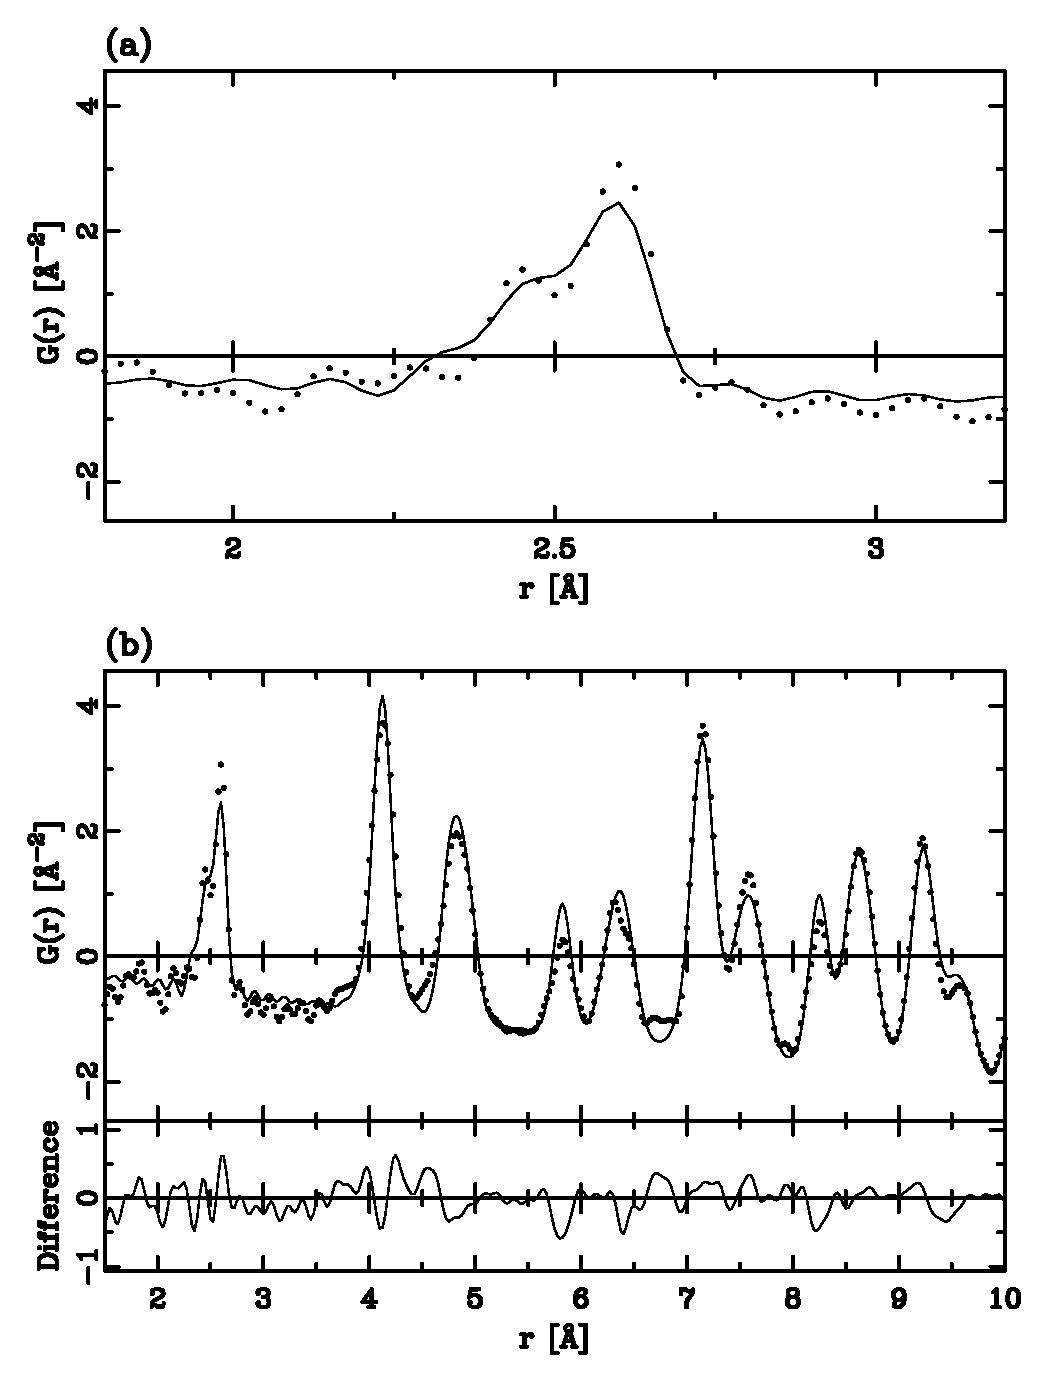
\includegraphics[scale=0.65, angle=0]{exa.1a.eps}
   \caption[Result of PDF refinement A of $In_{0.5}Ga_{0.5}As$]
           {Result of PDF refinement A of $In_{0.5}Ga_{0.5}As$.
            The solid line is the calculated PDF, the filled circles are
            the data. Panel (a) shows the region around the split first
            PDF peak and (b) shows the complete refinement range.
            A difference curve is plotted below the data.}
   \label{exa_fig1a}
\end{figure}

\footnotesize
\begin{MacVerbatim}
      1 reset
      2 read stru,in50.stru
      3 read data,x,45.0,0.0,in50.data
      4 #
      5 urf 5.
      6 cyc 100
      7 range 1,1.5,10.0
\end{MacVerbatim}
\normalsize

\noindent First we reset {\it PDFFIT} (line 1), read the starting
structure (line 2) and the data (line 3). Our starting structure
includes static nearest neighbor displacements to account for the
different $In$-$As$ and $Ga$-$As$ bond length. The atom
coordinates of the starting structure are listed below:

\footnotesize
\begin{MacVerbatim}
   GA         -0.00500000       -0.00350000       -0.00350000
   IN          0.00550000        0.50550002        0.50550002
   GA          0.49450001       -0.00550000        0.49450001
   IN          0.50449997        0.50449997        0.00450000
   AS          0.26499999        0.23500000        0.26499999
   AS          0.26499999        0.76499999        0.73500001
   AS          0.75599998        0.26199999        0.73600000
   AS          0.73699999        0.76300001        0.23700000
\end{MacVerbatim}
\normalsize

\noindent As one can see, half of the metal sites are occupied by
$In$, the other half by $Ga$. All atoms have been shifted from
their ideal position to accommodate the static displacement. The
positions shown could be refined using {\it PDFFIT}, however, this
is beyond the scope of this section. In the next part we assign
parameters for the lattice parameters $a=b=c$ (line 13--15) and
corresponding starting values (lines 17--19). Next the scaling
factor, $\sigma_{Q}$ and the dynamic correlation factor $\delta$
are assigned to their refinement parameters (lines 21--23) and
again starting values for those parameters need to be given (lines
25--27).

\footnotesize
\begin{MacVerbatim}
      8 #
      9 ###############################################################
     10 # Experimental and lattice parameters
     11 ###############################################################
     12 #
     13 par lat[1]=p[1],1.0
     14 par lat[2]=p[1],1.0
     15 par lat[3]=p[1],1.0
     16 #
     17 p[1]=lat[1]
     18 p[2]=lat[1]
     19 p[3]=lat[1]
     20 #
     21 par csca[1]=p[20],1.0
     22 par qsig[1]=p[21],1.0
     23 par delt[1]=p[22],1.0
     24 #
     25 p[20]=0.40
     26 p[21]=0.03
     27 p[22]=0.10
\end{MacVerbatim}
\normalsize

\noindent In the next segment we assign two parameters for the
isotropic temperature factors $U=U_{11}=U_{22}=U_{33}$ for the
metal site occupied by $In$ and $Ga$ as well as for $As$. This is
done in a similar fashion than for the $Ni$ example given in
chapter \ref{quick} by using {\tt do} loops. A scan be seen from
the structure file shown above, the first four atoms are the
metals ($In,Ga$) and atoms 5 to 8 are $As$, so the first loop
(line 33) loops over atoms 1--4, the second loop goes over numbers
5--8.

\begin{figure}[!bth]
   \centering
   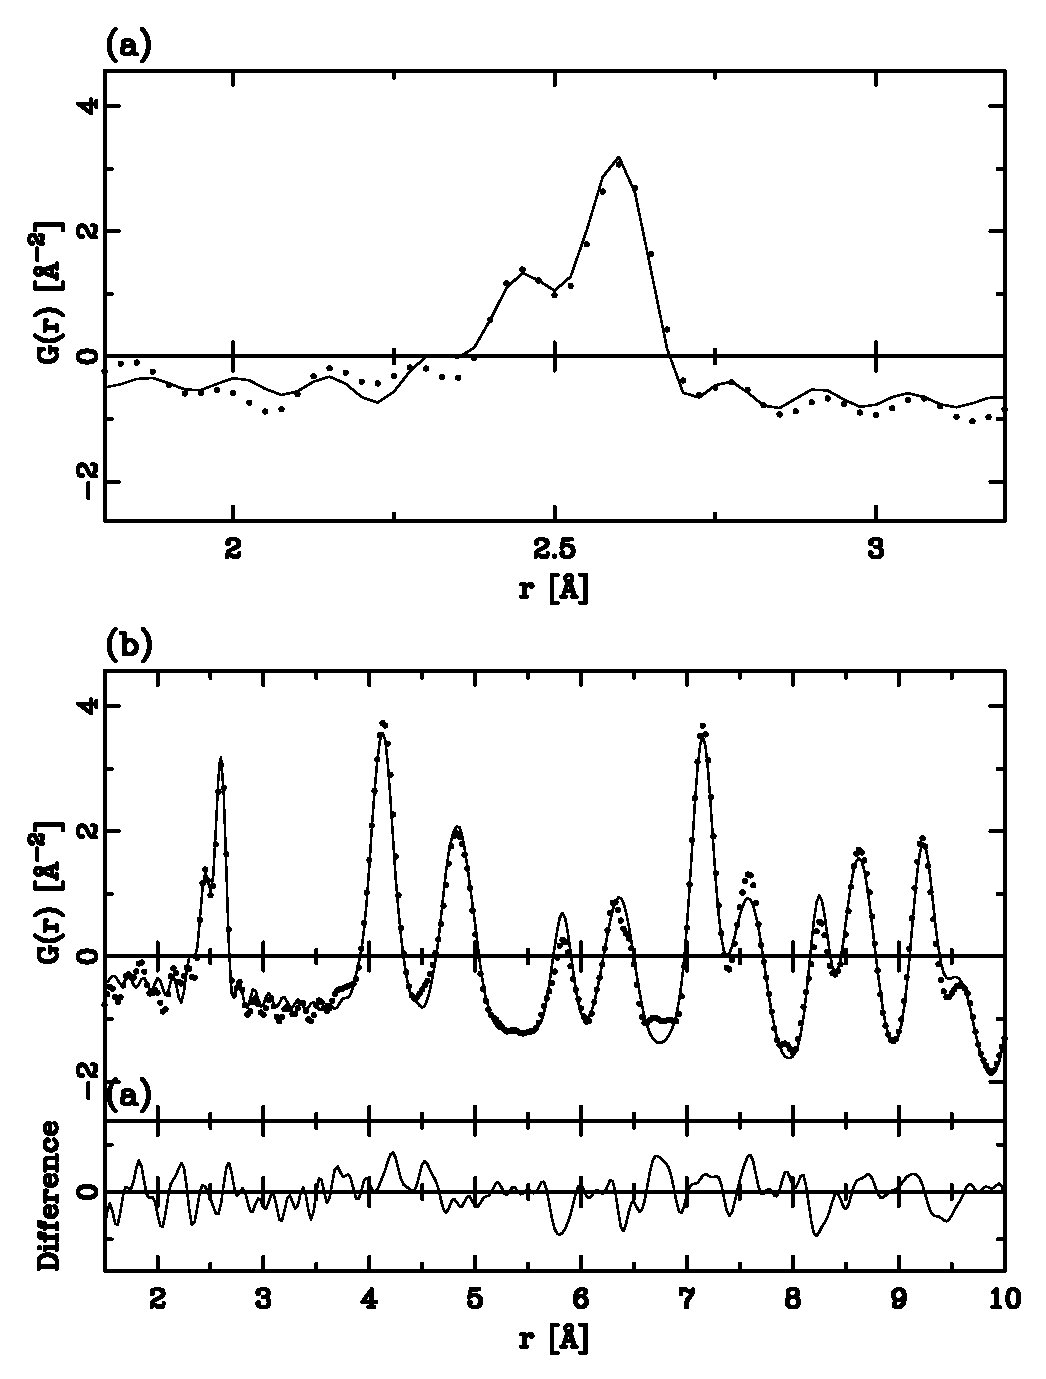
\includegraphics[scale=0.65, angle=0]{exa.1b.eps}
   \caption[Result of PDF refinement B of $In_{0.5}Ga_{0.5}As$]
           {Result of PDF refinement B of $In_{0.5}Ga_{0.5}As$.
            Details see caption of Figure \ref{exa_fig1a}.}
   \label{exa_fig1b}
\end{figure}

\footnotesize
\begin{MacVerbatim}
     28 #
     29 ###############################################################
     30 # Temperature factors
     31 ###############################################################
     32 #
     33 do i[1]=1,4
     34   par u[1,i[1]]=p[4],1.0
     35   par u[2,i[1]]=p[4],1.0
     36   par u[3,i[1]]=p[4],1.0
     37 enddo
     38 #
     39 do i[1]=5,8
     40   par u[1,i[1]]=p[5],1.0
     41   par u[2,i[1]]=p[5],1.0
     42   par u[3,i[1]]=p[5],1.0
     43 enddo
     44 #
     45 p[4]=u[1,1]
     46 p[5]=u[1,5]
\end{MacVerbatim}
\normalsize

\noindent After all parameter coding is done, we need to start the
refinement (line 47) and after the run is finished, we need to
save the results to individual files (lines 49--52).

\footnotesize
\begin{MacVerbatim}
     47 run
     48 #
     49 save pdf,1,in50.pdf
     50 save dif,1,in50.dif
     51 save stru,1,in50.rstr
     52 save res,in50.res
\end{MacVerbatim}
\normalsize

\noindent Inspection of Figure \ref{exa_fig1a} shows a reasonable
agreement when taking the complete $r$ range into account,
however, the split first neighbour peak shown in panel (a) of
Figure \ref{exa_fig1a} agrees rather badly with the observed PDF.
To understand this, we need to consider, that we have modeled
static displacements only for the nearest neighbour and
consequently only the width of the first PDF peak is completely
determined by thermal broadening whereas the other peaks are
determined by thermal as well as static displacements. The
dynamical correlation factor $\delta$ describes the $r$ dependence
of the PDF peak with according to the following empirical
equation:

\begin{equation}
  \sigma = \sigma` - \frac{\delta}{r^{2}}
\end{equation}

\noindent with $\sigma$ standing for the actual PDF peak width and
$\sigma'$ the width for uncorrelated motion, the value $\sigma$
converges to for high values of $r$. However, the parameter
$\delta$ is designed to take the correlated nature of thermal
motion into account. But in our case, we need a sharper transition
from the first peak which is purely thermal in origin and the
other peaks that contain thermal as well as static contributions.
To solve this problem, we sharpen the PDF peaks below a given
value $r_{cut}$ by a factor $\phi$ (see section \ref{fit_pwid} for
details. All we need to do, is to add the following lines to our
example macro:

\footnotesize
\begin{MacVerbatim}
     28a  par srat[1]=p[23],1.0
     28b  p[23]=0.3
     28c  rcut[1]=3.0
\end{MacVerbatim}
\normalsize

\noindent The ratio $\phi$ stored in the variable {\tt srat[s]} is
assigned to refinement parameter {\tt p[23]} (line 28a) and a
suitable starting value is set (line 28b). Furthermore, we need to
define the value of $r_{cut}$ or {\tt rcut[s]} for the
corresponding data set. This value determines below which value of
$r$ the PDF peak width is multiplied by $\phi$. The result of this
modified refinement can be seen in Figure \ref{exa_fig1b}. It is
obvious that the refinement describes the first PDF peak much
better, which is also reflected in the R-value of R=15.6\%
compared to R=19.1\% for the refinement without additional
sharpening.

%------------------------------------------------------------------------

\section{Example 2: Manganites\label{exa_mang}}

As a next example we will discuss a slightly more complicated
example, $LaMnO_{3}$. The structure is orthorhombic at room
temperature, space group $Pbnm$. Assuming one has an experimental
PDF, the first step is to obtain a starting structure. The data
used in this example were measured by G.H. Kwei and S.J.L.
Billinge on the special environment diffractometer (SEPD) at the
IPNS, Argonne. Unfortunately space group $Pbnm$ is a nonstandard
setting and the relations must be derived from space group $Pnma$
listed in the International Tables for Crystallography
\cite{tables} by cyclic permutation of the elements of the
relevant generators. Because we need this information later on,
the symmetrically equivalent positions are listed in Table
\ref{exa_tab2}.

\begin{table}[!htb]
\centering
\begin{tabular}{ccccc}
 (8d)& $x,y,z$
     & $x+\frac{1}{2},\overline{y}+\frac{1}{2},\overline{z}$
     & $\overline{x},\overline{y},z+\frac{1}{2}$
     & $\overline{x}+\frac{1}{2},y+\frac{1}{2},\overline{z}+\frac{1}{2}$
     \vspace{1mm} \\
     & $\overline{x},\overline{y},\overline{z}$
     & $\overline{x}+\frac{1}{2},y+\frac{1}{2},z$
     & $x,y,\overline{z}+\frac{1}{2}$
     & $x+\frac{1}{2},\overline{y}+\frac{1}{2},z+\frac{1}{2}$
     \vspace{2mm} \\
 (4c)& $x,y,\frac{1}{4}$
     & $x+\frac{1}{2},\overline{y}+\frac{1}{2},\frac{3}{4}$
     & $\overline{x},\overline{y},\frac{3}{4}$
     & $\overline{x}+\frac{1}{2},y+\frac{1}{2},\frac{1}{4}$
     \vspace{2mm} \\
 (4b)& $0,\frac{1}{2},0$
     & $\frac{1}{2},0,0$
     & $0,\frac{1}{2},\frac{1}{2}$
     & $\frac{1}{2},0,\frac{1}{2}$
\end{tabular}
\caption[Positions in space group $Pbnm$]
        {Symmetrically equivalent positions in space group $Pbnm$ for
         $Mn$ on (4b), $La,O$ on (4c) and $O$ on (8d).\label{exa_tab2}}
\end{table}

\noindent Using the same procedure as described in section
\ref{file_stru} we will use {\it DISCUS} to expand the structure
using the symmetry generators in space group $Pbnm$. The following
input file describes the structure as found in the literature
\citep{rohemo98}.

\footnotesize
\begin{MacVerbatim}
  title LaMnO3 - La (4c) - Mn (4b) - O (4c & 8d)
  spcgr Pbnm
  cell   5.5367   5.7473    7.6929   90.000000   90.000000   90.000000
  atoms
  LA         -0.007800        0.049000        0.250000     0.3400
  MN          0.000000        0.500000        0.000000     0.2100
  O           0.074500        0.487400        0.250000     0.5000
  O           0.725600        0.306600        0.038400     0.4300
\end{MacVerbatim}
\normalsize

\noindent Note that if we would use this structure file as input
for {\it PDFFIT} only those four atoms would be used. It is a
required step to use {\it DISCUS} to generate the other positions
or add them by hand. The expanded structure file that is used for
the refinement is shown below.

\footnotesize
\begin{MacVerbatim}
  title LaMnO3 - La (4c) - Mn (4b) - O (4c & 8d)
  spcgr Pbnm
  cell   5.5367   5.7473    7.6929   90.000000   90.000000   90.000000
  ncell        1,       1,       1,        20
  atoms
  LA           .992200         .049000         .250000      .3400
  LA           .492200         .451000         .750000      .3400
  LA           .007800         .951000         .750000      .3400
  LA           .507800         .549000         .250000      .3400
  MN           .000000         .500000         .000000      .2100
  MN           .500000         .000000         .000000      .2100
  MN           .000000         .500000         .500000      .2100
  MN           .500000         .000000         .500000      .2100
  O            .074500         .487400         .250000      .5000
  O            .574500         .012600         .750000      .5000
  O            .925500         .512600         .750000      .5000
  O            .425500         .987400         .250000      .5000
  O            .725600         .306600         .038400      .4300
  O            .225600         .193400         .961600      .4300
  O            .274400         .693400         .538400      .4300
  O            .774400         .806600         .461600      .4300
  O            .274400         .693400         .961600      .4300
  O            .774400         .806600         .038400      .4300
  O            .725600         .306600         .461600      .4300
  O            .225600         .193400         .538400      .4300
\end{MacVerbatim}
\normalsize

\noindent This structure file now contains all 20 atoms per unit
cell. Note that {\it DISCUS} could also have been used to create a
larger model structure, e.g. 2x1x1 unit cells. Note that per
convention {\it DISCUS} will transform the fractional coordinates
of all atoms within a single unit cell to the range 0 to 1. \par

After having the required input files, i.e. an experimental PDF and
a starting structure, one can start the refinement. In our example
we want to refine isotropic temperature factors as well as positions,
however, the symmetry constraints given by space group $Pbnm$ shall
be applied. The following sequence of commands is used for the refinement.
Obviously it is more convenient to prepare a text file with the commands
and start it as a macro in {\it PDFFIT} using the {\tt @} command. As before
the line numbers in the example here are for easy reference only and not
part of the actual input.

\footnotesize
\begin{MacVerbatim}
      1 reset
      2 read stru,lmo.stru
      3 read data,n,27.0,0.03,lmo.data
      4 #
      5 urf 5.0
      6 cyc 100
      7 range 1.0,15.0
\end{MacVerbatim}
\normalsize

\noindent After {\it PDFFIT} has been reset (line 1), the starting
structure (line 2) and PDF data (line 3) are read. The parameters
in line 3 identify the data to be obtained from neutron scattering
({\tt n}) with a maximum $Q$ value of $Q_{max}=27$\AA$^{-1}$. The
next parameters specifies the value for $\sigma_{Q}$ followed by
the name of the data file. For details about the file formats and
conversion tools refer to chapter \ref{file} of this manual. In
line 5 the magic number for the refinement is set to 5.0 (see
section \ref{fit_opt}). Next the maximum number of iterations is
set to 100, which is of course much larger than the number of
iteration we expect before the fit converges (or explodes). The
command {\tt range} (line 7) sets the range in real space used for
the refinement to 1.0 to 15.0\AA. The main part of the example
macro contains refinement parameter definitions. We start with
lattice parameters and some experimental parameters.

\footnotesize
\begin{MacVerbatim}
      8 #
      9 ###############################################################
     10 # Experimental and lattice parameters
     11 ###############################################################
     12 #
     13 par lat[1]=p[1],1.0
     14 par lat[2]=p[2],1.0
     15 par lat[3]=p[3],1.0
     16 #
     17 p[1]=lat[1]
     18 p[2]=lat[2]
     19 p[3]=lat[3]
     20 #
     21 par csca[1]=p[200],1.0
     22 par qsig[1]=p[201],1.0
     23 par delt[1]=p[202],1.0
     24 #
     25 p[200]=0.40
     26 p[201]=0.03
     27 p[202]=0.10
\end{MacVerbatim}
\normalsize

\noindent Lines 8--12 are simply a comment to make the macro file
easier to read. It is generally recommended to include descriptive
comments in refinement macros. Since our structure is
orthorhombic, we assign three parameters {\tt p[1],p[2]} and {\tt
p[3]} to refine the lattice parameters $a,b$ and $c$ stored in
variables {\tt lat[1], lat[2]} and {\tt lat[3]} (line 13--15). The
syntax of the command {\tt par} was already discussed in detail in
section \ref{fit_code}. The starting values for the parameters
{\tt p[1]} to {\tt p[3]} are set in lines 17--19. It is important
to assign each used refinement parameter a proper starting value
before starting the refinement. In lines 21--23 we assign
parameters to the scale factor $f_{p}$, the resolution parameter
$\sigma_{Q}$ and the dynamic correlation factor $\delta$. Again
each parameter needs a proper starting value (lines 25--27). The
choice which parameters {\tt p[n]} is assigned to which
experimental or structural parameter is completely up to the user.

\footnotesize
\begin{MacVerbatim}
     28 #
     29 ###############################################################
     30 # Temperature factors
     31 ###############################################################
     32 #
     33 do i[1]=1,4
     34   par u[1,i[1]]=p[4],1.0
     35   par u[2,i[1]]=p[4],1.0
     36   par u[3,i[1]]=p[4],1.0
     37 enddo
     38 #
     39 do i[1]=5,8
     40   par u[1,i[1]]=p[5],1.0
     41   par u[2,i[1]]=p[5],1.0
     42   par u[3,i[1]]=p[5],1.0
     43 enddo
     44 #
     45 p[4]=u[1,1]
     46 p[5]=u[1,5]
     47 #
     48 do i[1]=9,16
     49   par u[1,i[1]]=p[6],1.0
     50   par u[2,i[1]]=p[6],1.0
     51   par u[3,i[1]]=p[6],1.0
     52 enddo
     53 #
     54 do i[1]=17,20
     55   par u[1,i[1]]=p[7],1.0
     56   par u[2,i[1]]=p[7],1.0
     57   par u[3,i[1]]=p[7],1.0
     58 enddo
     59 #
     60 p[6]=u[1, 9]
     61 p[7]=u[1,17]
\end{MacVerbatim}
\normalsize

\noindent In out structure, we have atoms on four different
positions: $Mn$ on (4b), $La, O$ on (4c) and $O$ on (8d). The
program {\it PDFFIT} assigns numbers to each atom in the same
order they appear in the structure file. Inspecting the structure
file listed above, we find that atoms 1--4 are $Mn$, 5--8 are
$La$, 9--16 are the oxygens on position (4c) and finally atoms
17--20 are the oxygens on position (8d). The command sequence
above assigns an individual isotropic thermal parameter
$U=U_{11}=U_{22}=U_{33}$ to all four atom types (two for the
different oxygens). In this example we use {\tt do} loops for the
parameter assignment (see section \ref{fit_code}). The first loop
(line 33) goes over atoms 1 to 4 and assigns parameters {\tt
u[1,n], u[2,n]} and {\tt u[3,n]} a single refinement parameter
{\tt p[4]}. The same is done for the $La$ atoms in lines 39--43.
Next starting values are given to the parameters (lines 45--46).
The last part of this segment assigns isotropic temperature
factors to the two different oxygen sites in a similar way. \par

So far the example was quite straight forward and not really different
from the simple macro given in chapter \ref{quick}. Next we want to
refine the atom positions, but restricted to the space group $Pbnm$.
For $Mn$ we have no free positional parameter, for $La$ and oxygen on
position (4c) there are two refinable parameters $(x,y)$ and for
the oxygen on position (8d) all three coordinates can be refined.
The parameter coding for $La$ is show below:

\footnotesize
\begin{MacVerbatim}
     62 #
     63 ###############################################################
     64 # Positions (constrained)
     65 ###############################################################
     66 #
     67 # La on (4c)
     68 #
     69 par x[ 1]= 1.0+p[21], 1.0
     70 par y[ 1]= 0.0+p[22], 1.0
     71 par x[ 2]= 0.5+p[21], 1.0
     72 par y[ 2]= 0.5-p[22],-1.0
     73 par x[ 3]= 0.0-p[21],-1.0
     74 par y[ 3]= 1.0-p[22],-1.0
     75 par x[ 4]= 0.5-p[21],-1.0
     76 par y[ 4]= 0.5+p[22], 1.0
     77 #
     78 p[21]=-0.0078
     79 p[22]= 0.0490
\end{MacVerbatim}
\normalsize

\noindent The $x$ coordinate of atom one is assigned to parameter
{\tt p[21]} and $y$ is assigned {\tt p[22]}. In line 69 and 74 we
have added 1.0 to conform to the {\it DISCUS} convention that
fractional coordinates range from 0 to 1. The atom positions of
the other three $La$ atoms are calculated according to the
relations given in Table \ref{exa_tab2}. Note the sign of the
derivatives in this example ! The coding for the oxygens on site
(4c) is exactly the same (apart from $\pm$1.0) and shown below:

\footnotesize
\begin{MacVerbatim}
     80 #
     81 # O on (4c)
     82 #
     83 par x[ 9]=0.0+p[23], 1.0
     84 par y[ 9]=0.0+p[24], 1.0
     85 par x[10]=0.5+p[23], 1.0
     86 par y[10]=0.5-p[24],-1.0
     87 par x[11]=1.0-p[23],-1.0
     88 par y[11]=1.0-p[24],-1.0
     89 par x[12]=0.5-p[23],-1.0
     90 par y[12]=0.5+p[24], 1.0
     91 #
     92 p[23]= 0.0745
     93 p[24]= 0.4874
\end{MacVerbatim}
\normalsize

\noindent The coding for the oxygen atoms on site (8d) is slightly
longer since we change all three coordinates and have 8
symmetrically equivalent positions. However, following Table
\ref{exa_tab2} there should be no difficulty to understand the
following part of the {\it PDFFIT} macro.

\footnotesize
\begin{MacVerbatim}
     94 #
     95 # O on (8d)
     96 #
     97 par x[13]= 0.0+p[25], 1.0
     98 par y[13]= 0.0+p[26], 1.0
     99 par z[13]= 0.0+p[27], 1.0
    100 par x[14]=-0.5+p[25], 1.0
    101 par y[14]= 0.5-p[26],-1.0
    102 par z[14]= 1.0-p[27],-1.0
    103 par x[15]= 1.0-p[25],-1.0
    104 par y[15]= 1.0-p[26],-1.0
    105 par z[15]= 0.5+p[27], 1.0
    106 par x[16]= 1.5-p[25], 1.0
    107 par y[16]= 0.5+p[26], 1.0
    108 par z[16]= 0.5-p[27],-1.0
    109 par x[17]= 1.0-p[25],-1.0
    110 par y[17]= 1.0-p[26],-1.0
    111 par z[17]= 1.0-p[27],-1.0
    112 par x[18]= 1.5-p[25],-1.0
    113 par y[18]= 0.5+p[26], 1.0
    114 par z[18]= 0.0+p[27], 1.0
    115 par x[19]= 0.0+p[25], 1.0
    116 par y[19]= 0.0+p[26], 1.0
    117 par z[19]= 0.5-p[27],-1.0
    118 par x[20]=-0.5+p[25], 1.0
    119 par y[20]= 0.5-p[26],-1.0
    120 par z[20]= 0.5+p[27], 1.0
    121 #
    122 p[25]= 0.7256
    123 p[26]= 0.3066
    124 p[27]= 0.0384
\end{MacVerbatim}
\normalsize

\noindent Now the parameter coding is complete and the refinement
can be started using the command {\tt run} (line 125). After the
fit has converged, the results have to be stored. In line 127 the
resulting structure is saved to the file {\it lmo\_ref.stru}, next
the calculated PDF and its difference to the experimental data are
written to a file (lines 128--129) and finally the refinement
result is saved to the file {\it lmo\_ref.res}.

\footnotesize
\begin{MacVerbatim}
    125 run
    126 #
    127 save stru,1,lmo_ref.stru
    128 save pdf,1,lmo_ref.pdf
    129 save dif,1,lmo_ref.dif
    130 save res,lmo_ref.res
\end{MacVerbatim}
\normalsize

\begin{figure}[!bt]
   \centering
   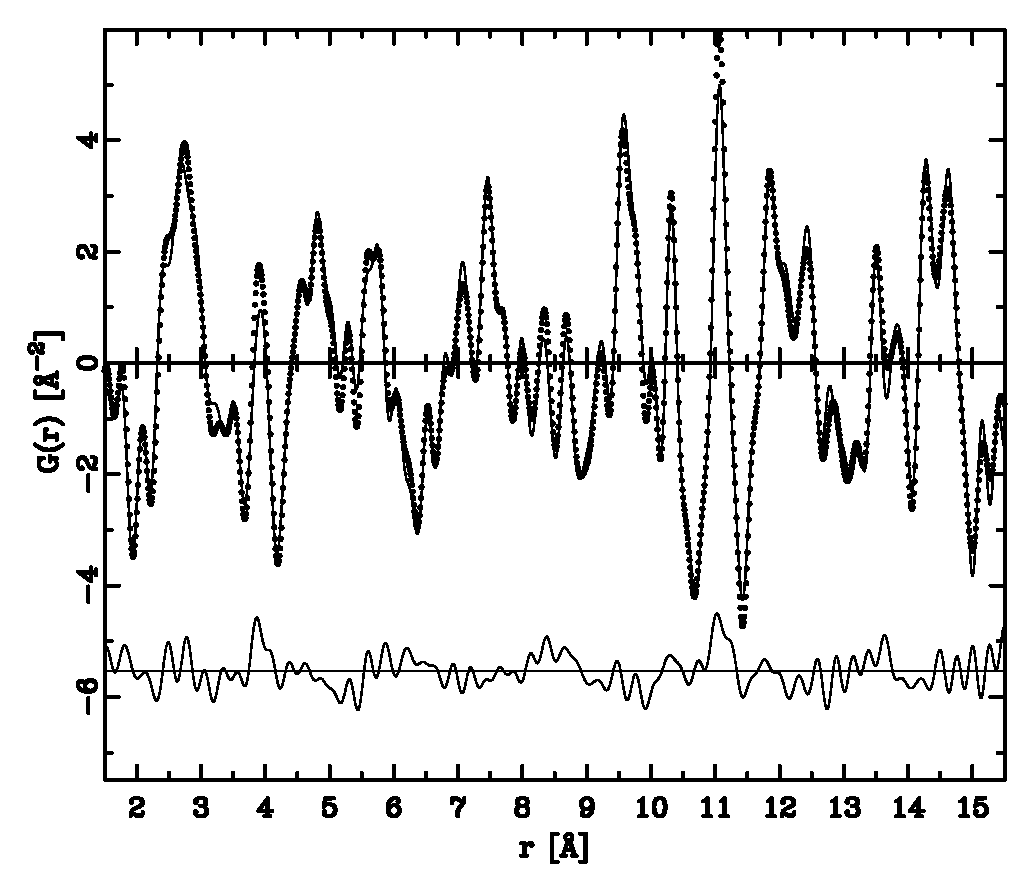
\includegraphics[scale=0.65, angle=0]{exa.2.eps}
   \caption[Result of PDF refinement of $LaMnO_{3}$]
           {Result of PDF refinement of $LaMnO_{3}$. The solid line is the
            calculated PDF, the filled circles are the data. A difference
            curve is plotted below the data.}
   \label{exa_fig2}
\end{figure}

\noindent The result of the refinement is shown in Figure
\ref{exa_fig2}. The next step one might be interested in is to
refine the positions of the oxygen atoms without the symmetry
restrictions imposed by space group $Pbnm$ since the $Mn-O$
octahedra might have {\it locally} a different symmetry. One way
of doing this is to construct different constraint equations based
on geometrical considerations. Alternatively one could refine all
oxygen coordinates individually. One possible parameter coding
shown below is quite similar to the coding of the thermal factors
above.

\footnotesize
\begin{MacVerbatim}
      1 ###############################################################
      2 # Positions O1 and O2 (free)
      3 ###############################################################
      4 do i[1]=9,12
      5   par x[i[1]]=p[i[1]*3+51],1.0
      6   par y[i[1]]=p[i[1]*3+52],1.0
      7 #
      8   p[i[1]*3+51]=x[i[1]]
      9   p[i[1]*3+52]=y[i[1]]
     10 enddo
     11 #
     12 do i[1]=13,20
     13   par x[i[1]]=p[i[1]*3+51],1.0
     14   par y[i[1]]=p[i[1]*3+52],1.0
     15   par z[i[1]]=p[i[1]*3+53],1.0
     16 #
     17   p[i[1]*3+51]=x[i[1]]
     18   p[i[1]*3+52]=y[i[1]]
     19   p[i[1]*3+53]=z[i[1]]
     20 enddo
\end{MacVerbatim}
\normalsize

\noindent Note that we are not refining the $z$ value of the
oxygen sitting on site (4c), although in principle one could try
even that. It is important to understand, that the PDF probes the
{\it local} structure. By selecting different ranges in $r$ one
has control over the length scale on which the refined {\it local}
arrangement occurs. For further reading refer to the references
given in the introduction of this users guide.

%------------------------------------------------------------------------

\section{Example 3: Nickel using multiple data sets\label{exa_nimul}}

In this section a combined refinement of two data sets for $Ni$
will be shown. The first data set was already used in the $Ni$
example shown in chapter \ref{quick} with a value of
$Q_{max}=22$\AA$^{-1}$. The second data set is taken from the
Billinge group (Michigan State University) diffractometer using a
conventional X-ray tube as source. Using MoK$\alpha$ radiation a
value of $Q_{max}=16$\AA$^{-1}$ could be reached. The refinement
macro file is listed below:

\begin{figure}[!tb]
   \centering
   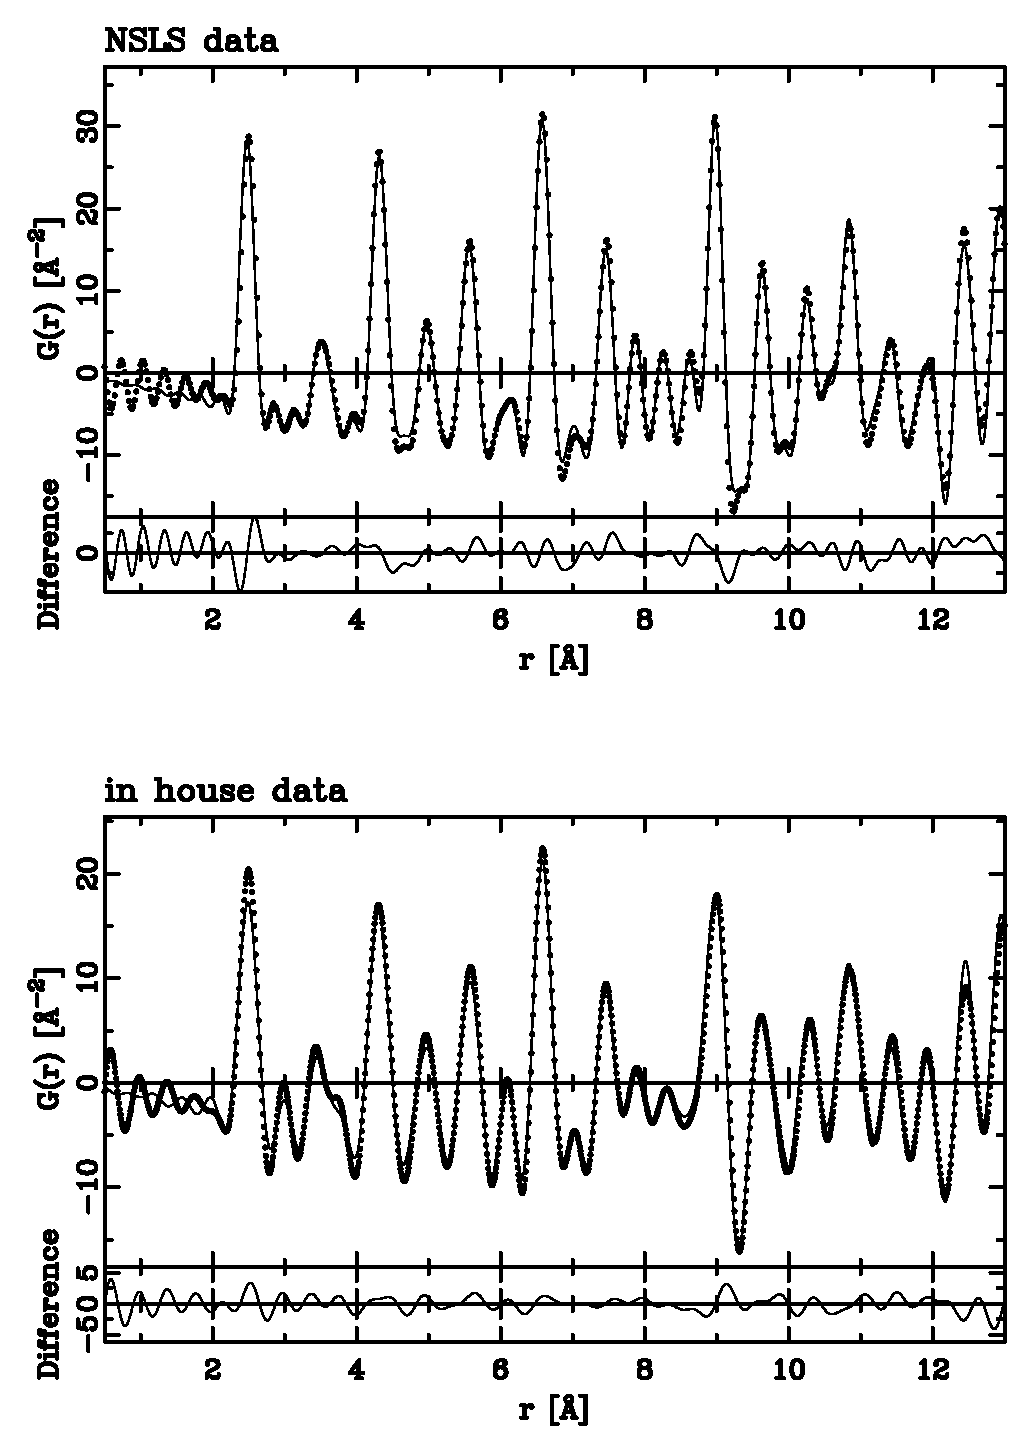
\includegraphics[scale=0.65, angle=0]{exa.3.eps}
   \caption[Result of PDF refinement of two data sets of $Ni$]
           {Result of PDF refinement of two data sets of $Ni$.
            The solid line is the calculated PDF, the filled circles are
            the data. The top panel shows synchrotron (NSLS) data,
            the bottom panel shows data from a in house X-ray source.
            A difference curve is plotted below the data.}
   \label{exa_fig3}
\end{figure}

\footnotesize
\begin{MacVerbatim}
      1 reset
      2 read stru,ni.stru
      3 read data,x,22.0,0.0,ni-nsls.data
      4 read data,x,16.0,0.0,ni-inhs.data
      5 #
      6 range 1,0.5,13.0
      7 range 2,0.5,13.0
      8 #
      9 par dsca[1]=p[10],1.0
     10 par dsca[2]=p[11],1.0
     11 par qsig[1]=p[12],1.0
     12 par qsig[2]=p[13],1.0
     13 #
     14 par delt[1]=p[14],1.0
     15 #
     16 p[10]=1.50
     17 p[11]=1.00
     18 p[12]=0.03
     19 p[13]=0.03
     20 p[14]=0.10
\end{MacVerbatim}
\normalsize

\noindent The first two lines are as before, resetting {\it
PDFFIT} and reading the structure file. Now we need to issue a
{\tt read} command for each data set. Note the different file
names and values for $Q_{max}$ in lines 3 and 4. There are two
data set dependent parameters, the scaling factor $f_{s}$ and the
resolution factor $\sigma_{Q}(s)$. One refinement parameter is
assigned to each one for each of the two data sets (lines 9--12).
Note that in previous examples we have used the scale factor
$f_{p}$ corresponding to the structural phase $p$. In cases where
we have only {\it one} phase and {\it one} data set we are free to
choose which scale factor to refine. Now the scale factors related
to the different data sets must be used. The starting values for
the different defined refinement parameters are set in lines
16--20.

\footnotesize
\begin{MacVerbatim}
     21 #
     22 ###########################################################
     23 # Refining lattice parameters and thermal factors
     24 ###########################################################
     25 #
     26 par lat[1]=p[1],1.0
     27 par lat[2]=p[1],1.0
     28 par lat[3]=p[1],1.0
     29 #
     30 do i[1]=1,n[1]
     31   par u[1,i[1]]=p[2],1.0
     32   par u[2,i[1]]=p[2],1.0
     33   par u[3,i[1]]=p[2],1.0
     34 enddo
     35 #
     36 p[1]=lat[1]
     37 p[2]=u[1,1]
     38 #
     39 ###########################################################
     40 # Running the refinement and saving results
     41 ###########################################################
     42 #
     43 run
     44 #
     45 save pdf,1,ni-nsls.calc
     46 save pdf,2,ni-inhs.calc
     47 save dif,1,ni-nsls.dif
     48 save dif,2,ni-inhs.dif
     49 save stru,1,ni_ref.stru
     50 save res,ni_ref.out
\end{MacVerbatim}
\normalsize

\noindent In this last part of the macro, we define refinement
parameters for the lattice parameters $a=b=c$ and the isotropic
thermal factor for the $Ni$ atom. This is identical to the quick
example given in chapter \ref{quick}, the only difference is that
one needs to save the calculated PDF and the difference between
observed and calculated PDF for each data set separately (lines
45--48). The results for the synchrotron as well as the in-house
data can be seen in Figure \ref{exa_fig3}. Note that {\it PDFFIT}
outputs only the total R-value of the refinement. Individual
R-values for the different data sets or for a specific region in
$r$ can be obtained using the {\it PDFFIT} function {\tt rval}
(see section \ref{func}).

%------------------------------------------------------------------------

%------------------------------------------------------------------------
% Chapter:  Misc. functions
%------------------------------------------------------------------------

\chapter{Calculating structural properties \label{misc}}

{\it PDFFIT} offers like {\it DISCUS} the intrinsic functions
{\tt blen} and {\tt bang} to calculate the bond length and bond
angles between atoms or general positions within the model
crystal. However, {\it PDFFIT} allows the user to calculated
bond length and bond angles with standard deviations propagated
from the uncertainties of lattice parameters and positions obtained
during the refinement

%------------------------------------------------------------------------

\section{Calculating single bond lengths and angles \label{misc_simp}}

The bond length between any two atoms within the structure can simply
be calculated using the command {\tt blen} followed by the two atom
numbers. The following example calculates the distance between the
atoms {\tt 5} and {\tt 9}:

\footnotesize
\begin{MacVerbatim}
   pdffit > blen 5,9
       MN (#    5) -    O (#    9)   =   1.965(5) A
\end{MacVerbatim}
\normalsize

\noindent The names of the two selected atoms and distance is
given. If the standard deviations of the lattice parameters or the
positions of the atoms are not zero, the standard deviation of the
bond length is given as well. As usual the standard deviation is
given in round brackets after the last significant digit. In our
example the bond length is $1.965 \pm 0.005$\AA. The bond angle
defined by three atoms can be calculated in a similar way using
the command {\tt bang} as demonstrated below:

\footnotesize
\begin{MacVerbatim}
   pdffit > bang 9,5,13
       O (#    9) -   MN (#    5) -    O (#   13)   =   74.1(9) degrees
\end{MacVerbatim}
\normalsize

\noindent It should be noted, that these functions calculates the
direct distance between the given atoms, although the same atom
might be closer to a given atom in a neighbouring unit cell. No
periodic boundary conditions are applied. In order to obtain a
specific bond length or angle it might be necessary to modify the
atom coordinates by $\pm 1$. This can simply be done using the
corresponding variables, e.g. {\tt x[1]=x[1]+1.0}. Note that this
is actually modifying the current structure. Alternatively one can
compute all bond length in a given interval as discussed in the
next section.

%------------------------------------------------------------------------

\section{Calculating multiple bond lengths \label{misc_mult}}

The command {\tt blen} allows one to calculate all bond length
between selected atom types in a given interval. This can be
useful to monitor a specific bond length. In the following example
all $Mn-O$ bonds within a range of $1.8$ and $2.4$\AA\ are
calculated.

\footnotesize
\begin{MacVerbatim}
  pdffit > blen mn,o,1.8,2.4
   Bond lengths found in current phase :
     MN (#    5) -    O (#    9)   =          1.965(5) A
     MN (#    5) -    O (#   13)   =           1.93(1) A
     MN (#    5) -    O (#   18)   =           2.15(1) A
     MN (#    5) -    O (#   14)   =           2.15(1) A
     MN (#    5) -    O (#   17)   =           1.93(1) A
     MN (#    5) -    O (#   11)   =          1.965(5) A

     MN (#    6) -    O (#   13)   =           2.15(1) A
     MN (#    6) -    O (#   12)   =          1.965(5) A
     MN (#    6) -    O (#   18)   =           1.93(1) A
     MN (#    6) -    O (#   10)   =          1.965(5) A
     MN (#    6) -    O (#   14)   =           1.93(1) A
     MN (#    6) -    O (#   17)   =           2.15(1) A

     MN (#    7) -    O (#    9)   =          1.965(5) A
     MN (#    7) -    O (#   15)   =           1.93(1) A
     MN (#    7) -    O (#   20)   =           2.15(1) A
     MN (#    7) -    O (#   11)   =          1.965(5) A
     MN (#    7) -    O (#   16)   =           2.15(1) A
     MN (#    7) -    O (#   19)   =           1.93(1) A

     MN (#    8) -    O (#   10)   =          1.965(5) A
     MN (#    8) -    O (#   19)   =           2.15(1) A
     MN (#    8) -    O (#   20)   =           1.93(1) A
     MN (#    8) -    O (#   12)   =          1.965(5) A
     MN (#    8) -    O (#   15)   =           2.15(1) A
     MN (#    8) -    O (#   16)   =           1.93(1) A
\end{MacVerbatim}
\normalsize

\noindent As one can see around each of the four $Mn$ in the unit
cell we find six oxygens forming an octahedra. In this mode of the
command {\tt blen} periodic boundary conditions are applied in the
same way as for the calculation of the PDF and as a result
distances to atoms outside the structural box (or unit cell) are
also found.
\par

The command {\tt blen} might also be used to identify which atom
pairs contribute to a given PDF peak. Assume the peak in question
is between 3.5 and 3.6\AA. Simply enter the command {\tt blen
all,all,3.5,3.6} and {\it PDFFIT} will list all atom pairs that
are separated by a distance between 3.5 and 3.6\AA.

%------------------------------------------------------------------------


%------------------------------------------------------------------------
% Appendices
%------------------------------------------------------------------------

\appendix
%------------------------------------------------------------------------
% Chapter:  Appendix A
%------------------------------------------------------------------------

\chapter{Computational Details \label{app-deriv}}

Here we give the details of the computation of the model PDF $G(r)$. In
the introduction we defined $G(r)$ as follows:

\begin{equation}
  G(r) = \frac{1}{r} \sum_{i}\sum_{j} \left [
         \frac{b_{i}b_{j}}{\langle b \rangle ^{2}}
         \delta (r - r_{ij}) \right ]   - 4 \pi r \rho_{0}
  \label{eq_gr}
\end{equation}

As we discussed already in this manual, the sums go over all atoms
within the model crystal and $r_{ij}$ is the separation distance
between atoms $i$ and $j$. The value $b_{i}$ is the scattering length
for atom $i$ and $\langle b \rangle$ is the average scattering length
of the model crystal. Finally $\rho_{0}$ is the number density. \par

As we have seen in the introduction to this users guide, the
experimental PDF is obtained by Fourier transform of the reduced
structure factor. However, the accessible range in $Q$ is limited by
$Q_{max}$. This can be described by a multiplication of the
structure factor up to infinity with a step function cutting off at
$Q=Q_{max}$ resulting in the convolution of the PDF with the Fourier
transform $C(r)$ of the step function. {\it PDFFIT} models the
finite $Q$-range by convoluting the model PDF $G(r)$ with

\begin{equation}
  C(r) = \frac{\sin(Q_{max} \cdot r)}{r}
  \label{eq_sinc}
\end{equation}

In the following section we will omit this convolution and discuss how
$G(r)$ and the partial derivatives with respect to the refinement
parameters, $\partial G(r)/ \partial p_{n}$, are actually calculated.

%------------------------------------------------------------------------

\section{Calculating the PDF}

The program {\it PDFFIT} refines the function $G(r)$ at discreet
values of $r=r_{k}$ for an experimental dataset $s$. Thus our
equation for the model PDF becomes:

\begin{equation}
  G(r_{k},s) = f_{s} B_{k}(s)
               \sum_{p=1}^{P} f_{p} S_{p}(r_{k},s_{i}) G_{p}(r_{k},s)
  \label{eq_grk}
\end{equation}

\noindent
with

\begin{eqnarray}
  G_{p}(r_{k},s)  & = & \frac{1}{N_{p}r_{k}}
                        \sum_{i}\sum_{j} \left [ A_{ij}(p) \cdot
                        T_{ij}(r_{k},p) \right ] - 4\pi r_{k}\rho_{0}(p) \\
  \label{eq_grkp}
  B_{k}(s)        & = & \exp \left [ - \frac{(r_{k}\sigma_{Q}(s))^{2}}
                        {2}\right ] \\
  \label{eq_bk}
  A_{ij}(p)       & = & \frac{c_{i}(p)c_{j}(p)b_{i}b_{j}}
                        {\langle b \rangle ^{2}}
  \label{eq_aij}           \\
  T_{ij}(r_{k},p) & = & \frac{1}{\sqrt{2\pi}\sigma_{ij}(p)}
                        \exp \left [ - \frac{(r_{k}-r_{ij}(p))^{2}}
                        {2 \sigma_{ij}^{2}(p)} \right ]
                        \left [ 1 + \left ( \frac{r_{k} - r_{ij}}{r_{ij}}
                        \right ) \right ]
  \label{eq_tij}
\end{eqnarray}

\noindent where $S_{p}(r_{k},s_{i})$ is a dampening function for
finite nano-particles discussed in the next section. $f_{s}$ stands
for the overall scale factor and $B_{k}(s)$ is the experimental
resolution factor for data set $s$. The first sum in (\ref{eq_grk})
is over the different structural phases $p$ in a multi phase
refinement. The relative abundance of each phase $p$ is given by
$f_{p}$. $G_{p}(r_{k},s)$ is the model PDF for a single phase $p$
given in (\ref{eq_grkp}). These values are actually stored in an
array after the PDF is calculated. The indices $i$ and $j$ sum over
all atoms within the structural phase $p$ or in other words we sum
over all atom {\it pairs} in that phase. The contribution of each
pair of atoms $i$ and $j$ is weighted with a factor $A_{ij}(p)$
which depends on the scattering length $b_{i}$ and concentration
$c_{i}$ of both atoms. The average scattering length for the sample
({\bf summed over all phases}) is $\langle b \rangle =
\sum_{i}c_{i}b_{i}/N_{p}$. The average number density is given by
$\rho_{0}(p) = N_{p}/V_{p}$ where $N_{p} = \sum_{i}c_{i}$ is the
number of atoms within phase $p$ and $V_{p}$ is the volume of the
unit cell in \AA$^{3}$. The calculation of $V_{p}$ is presented
later in this section. \par

The final term in (\ref{eq_grk}) we need to discuss is
$T_{ij}(r_{k},p)$. Generally there are two different ways to
account for displacements (either thermal or static) from the
average position. First one can use a large enough model
containing the desired displacements and perform an ensemble
average. This is the method used by the program {\it DISCUS} where
thermal displacements can be introduced according to a given
(isotropic) Debye-Waller factor. Secondly one can convolute each
contribution given by $\delta (r - r_{ij})$ in (\ref{eq_gr}) with
a modified Gaussian $T_{ij}(r_{k},p)$ accounting for the
displacements. The deviation from a Gaussian shape is caused by
anisotropic averaging and discussed in detail in \cite{thlele02}.
The width of the function $T_{ij}$ is given by the anisotropic
thermal factors $U_{lm} = \langle u_{l}u_{m} \rangle$ of atoms $i$
and $j$. Furthermore the $\sigma_{ij}(p)$ shows an $r$-dependence
given in (\ref{eq_sharp}). Note that this definition has been
extended since version 1.2 of PDFFIT. In some cases an additional
sharpening of the PDF peaks below a user defined cutoff value,
$r_{cut}$ needs to be introduced (see \ref{fit_pwid} for details).
This is done in (\ref{eq_cut}).

\begin{equation}
  \sigma_{ij}(p) = \phi(r_{ij},p) \cdot
                   \sqrt {\sigma_{ij}^{'2}(p) -
                          \frac{\delta(p)}{r_{ij}^{2}(p)} -
                          \frac{\gamma(p)}{r_{ij}(p)} +
                          \alpha^{2}(s) r_{ij}^{2}(p)}
  \label{eq_sharp}
\end{equation}

\noindent
with

\begin{equation}
  \phi(r_{ij},p) = \left \{ \begin{array}{ll}
                    \phi_{0}(p) & \mbox{for $r_{ij} < r_{cut}$} \\
                    1.0         & \mbox{otherwise} \\
                    \end{array} \right .
  \label{eq_cut}
\end{equation}

\noindent
and

\begin{equation}
  \sigma'_{ij}(p) = \frac{1}{|r_{ij}|} \sqrt{\sum_{l,m=1}^{3} \left[
                    r^{l}_{ij}(p)r^{m}_{ij}(p) (U_{lm}(i) + U_{lm}(j))
                    \right ]}
  \label{eq_therm}
\end{equation}

\noindent
with $r^{l}_{ij}$ standing for the $l$-th component of the difference
vector between atoms $i$ and $j$. Note that so far $r_{ij}$ referred to
a scalar, the distance between the atoms without any directional
information. \par

The last piece of the puzzle is the relation between $r_{ij}(p)$ and
$V_{p}$ and the lattice parameters $a,b,c,\alpha,\beta$ and $\gamma$.
{\it PDFFIT} works with fractional coordinates, i.e. in units
of the unit cell. However, to calculate the distance between two atoms,
the difference vector must be converted to \AA. A helpful concept when
dealing with non-orthogonal coordinate systems is the so-called
{\it metric tensor}, $g_{ij}$, which is defined as

\begin{equation}
   g_{ij} = {\bf{a}}_{i} \cdot {\bf{a}}_{j} =
   \left ( \begin{array}{ccc}
           a^{2}         & ab \cos\gamma & ac \cos\beta  \\
           ab \cos\gamma & b^{2}         & bc \cos\alpha \\
           ac \cos\beta  & bc \cos\alpha & c^{2}
           \end{array} \right )
   \label{eq_metric}
\end{equation}

\noindent
with $\bf{a}_{i}$ describing the basis vectors of the crystal lattice
in an orthonormal system. Using this metric tensor, the scalar
product of two vectors $\bf{u}$ and $\bf{v}$ is simply ${\bf{uv}}
= \sum_{ij} u_{i}v_{j}g_{ij}$ or \begin{math} V_{p} = abc
[1 - \cos^{2}\alpha - \cos^{2}\beta - \cos^{2}\gamma + 2 \cos\alpha
\cos\beta \cos\gamma]^{\frac{1}{2}} \end{math} which is simply the
determinant of the metric tensor $g_{ij}$. \par

Let us assume we want to calculate the distance between the atoms $i$
and $j$ on positions ${\bf u}_{i}$ and ${\bf u}_{j}$ in the crystal
system (We will omit the reference to phase $p$ is this part). Now the
difference vector still in fractional coordinates is simply
${\bf d}_{ij} = {\bf u}_{j} - {\bf u}_{i}$. In order to get the
components $r^{l}_{ij}$ needed to calculate $\sigma'_{ij}$ in (\ref
{eq_therm}), we simply multiply with the corresponding lattice parameter:

\begin{equation}
  r^{1}_{ij} = a d^{1}_{ij}, \;
  r^{2}_{ij} = b d^{2}_{ij}, \;
  r^{3}_{ij} = c d^{3}_{ij}
  \label{eq_met1}
\end{equation}

\noindent
The length of the difference vector in \AA\ is given by
$r_{ij} = [{\bf d}_{ij} \cdot {\bf d}_{ij}] ^{\frac{1}{2}}$ which can
be written as follows using (\ref{eq_metric}):

\begin{eqnarray}
  r_{ij} & = & [ a^{2} d^{2}_{ij_{x}} +
                 b^{2} d^{2}_{ij_{y}} +
                 c^{2} d^{2}_{ij_{z}} + \nonumber \\
         &   &   2 ab \cos\gamma d_{ij_{x}}d_{ij_{y}} +
                 2 ac \cos\beta  d_{ij_{x}}d_{ij_{z}} +
                 2 bc \cos\alpha d_{ij_{y}}d_{ij_{z}} ] ^{\frac{1}{2}}
  \label{eq_met2}
\end{eqnarray}

Now we have all necessary relationships to calculate $G(r_{k},s)$ from
the experimental and structural parameters we might want to refine.
The needed analytical derivatives are given in the next section and the
actual parameter names used by {\it PDFFIT} are listed in the last
section of this appendix.

%------------------------------------------------------------------------

\section{Particle size envelopes}

With the possibility to measure and model PDFs over a wide range in
distances $r$, the finite size of nano-particles requires an extra
envelope function $S_{p}(r_{k},s_{i})$ that will depend on the
shape, size and size distribution of the measured particles. For
long range ordered crystals, this factor simply becomes unity. The
parameters $s_{i}$ are the refinable quantities defining the shape,
size and distribution.

%------------------------------------------------------------------------

\subsection*{Sphere}

At the moment only spherical particles can be simulated. In this
case the only refinable parameter, $s_{1}=R$, is the radius of the
particle and the envelope function becomes\cite{hoprco06} :

\begin{equation}
  S_{p}(r_{k},R) = \left ( 1 - \frac{3} {4} \left ( \frac{r_{k}}{R} \right )
                             + \frac{1}{16} \left ( \frac{r_{k}}{R} \right )^{3}
                          \right ) \Theta (2R - r_{k})
  \label{eq_shape_sphere}
\end{equation}

\noindent with  $\Theta(x)=0$ for $x<0$ and $\Theta(x)=1$ for $x
\geq 0$. More shapes and distributions will be added as their
analytical expression become available.

%------------------------------------------------------------------------

\section{Partial derivatives}

It should be noted that the derivatives given in this section
actually need to be convoluted with the function given in
(\ref{eq_sinc}) as well since $\partial (G(r,p) * C(r)) / \partial p
= (\partial G(r,p) / \partial p) * C(r)$.

\subsection*{Scale factors}

The derivatives with respect to the two scale factors $f_{s}$ and
$f_{p}$ are straight forward and listed below:

\begin{eqnarray}
  \frac{\partial G(r_{k},s)}{\partial f_{s}} & = &
     B_{k}(s) \sum_{p=1}^{P} f_{p} S_{p}(r_{k},s_{i}) G_{p}(r_{k},s) \\
  \frac{\partial G(r_{k},s)}{\partial f_{p}} & = &
     f_{s}B_{k}(s) S_{p}(r_{k},s_{i}) G_{p}(r_{k},s)
  \label{eq_d/ds}
\end{eqnarray}

%------------------------------------------------------------------------

\subsection*{Experimental resolution factor}

The experimental resolution $\sigma_{Q}$ only appears in $B_{k}(s)$,
thus the derivative is simply:

\begin{equation}
  \frac{\partial G(r_{k},s)}{\partial \sigma_{Q}(s)} =
     - r_{k}^{2} \sigma_{Q}(s) \; f_{s}B_{k}(s)
                 \sum_{p=1}^{p} f_{p} S_{p}(r_{k},s_{i}) G_{p}(r_{k},s)
  \label{eq_d/dsq}
\end{equation}

%------------------------------------------------------------------------

\subsection*{Quadratic dynamic correlation factor}

The dynamic correlation factor $\delta(p)$ appears only in $T_{ij}
(r_{k},p)$ where $\sigma_{ij}(p)$ appears. Thus we can rewrite the
derivative for a given phase $p$ (we omit the reference to $p$ in
the following equations) as follows:

\begin{equation}
  \frac{\partial G(r_{k},s)}{\partial \delta} =
    \frac{f_{s}f_{p} S_{p}(r_{k},s_{i}) B_{k}(s)}{N_{p}r_{k}} \sum_{i} \sum_{j}
    A_{ij} \frac{\partial T_{ij}(r_{k})}{\partial \delta}
  \label{eq_d/delta1}
\end{equation}

\noindent
with

\begin{eqnarray}
  \frac{\partial T_{ij}(r_{k})}{\partial \delta} & = &
    \frac{\partial T_{ij}(r_{k})}{\partial \sigma_{ij}}
    \frac{\partial \sigma_{ij}} {\partial \delta} \nonumber \\
  & = & \frac{T_{ij}(r_{k})}{\sigma_{ij}}
    \left [\frac{(r_{k} - r_{ij})^{2}}{\sigma_{ij}^{2}} - 1 \right ]\cdot
    \frac{- \phi^{2}(r_{ij})}{2 r_{ij}^{2} \sigma_{ij}}
  \label{eq_d/delta2}
\end{eqnarray}

\noindent
which gives the final result for the derivative of

\begin{equation}
  \frac{\partial G(r_{k},s)}{\partial \delta} =
    - \frac{f_{s}f_{p} S_{p}(r_{k},s_{i}) B_{k}(s)}{N_{p}r_{k}} \sum_{i} \sum_{j}
      \frac{\phi^{2}(r_{ij})A_{ij}(p)T_{ij}(r_{k})}{2 r_{ij}^{2} \sigma^{2}_{ij}}
      \left [ \frac{(r_{k} - r_{ij})^{2}}{\sigma_{ij}^{2}} - 1
      \right ]
  \label{eq_d/delta3}
\end{equation}

%------------------------------------------------------------------------

\subsection*{Linear dynamic correlation factor}

The linear correlation factor $\gamma(p)$ appears only where
$\sigma_{ij}$ appears. Similar to (\ref{eq_d/delta1}) we find
using

\begin{equation}
  \frac{\partial \sigma_{ij}}{\partial \gamma}=
  \frac{- \phi^{2}(r_{ij})}{2  r_{ij} \sigma_{ij}}
  \label{eq_d/gamma1}
\end{equation}

\noindent which gives the resulting expression of

\begin{equation}
  \frac{\partial G(r_{k},s)}{\partial \gamma} =
    - \frac{f_{s}f_{p} S_{p}(r_{k},s_{i}) B_{k}(s)}{N_{p}r_{k}} \sum_{i} \sum_{j}
      \frac{\phi^{2}(r_{ij})A_{ij}(p)T_{ij}(r_{k})}{2 r_{ij} \sigma^{2}_{ij}}
      \left [ \frac{(r_{k} - r_{ij})^{2}}{\sigma_{ij}^{2}} - 1
      \right ]
  \label{eq_d/gamma2}
\end{equation}

%------------------------------------------------------------------------

\subsection*{Resolution broadening factor}

The resolution broadening $\alpha(s)$ appears only where
$\sigma_{ij}$ appears. We omit the reference to $s$ in the
following equations for clarity. Similar to (\ref{eq_d/delta1}) we
find using

\begin{equation}
  \frac{\partial \sigma_{ij}}{\partial \alpha}=
  \frac{\alpha \phi^{2}(r_{ij}) r_{ij}^{2}}{\sigma_{ij}}
  \label{eq_d/alpha1}
\end{equation}

\noindent which gives the resulting expression of

\begin{equation}
  \frac{\partial G(r_{k},s)}{\partial \gamma} =
      \frac{f_{s}f_{p} S_{p}(r_{k},s_{i}) B_{k}(s)}{N_{p}r_{k}} \sum_{i} \sum_{j}
      \frac{\alpha \phi^{2}(r_{ij}) r_{ij}^{2}
            A_{ij}(p)T_{ij}(r_{k})}{\sigma^{2}_{ij}}
      \left [ \frac{(r_{k} - r_{ij})^{2}}{\sigma_{ij}^{2}} - 1
      \right ]
  \label{eq_d/alpha2}
\end{equation}

%------------------------------------------------------------------------

\subsection*{Peak with ratio}

The parameter $\phi_{0}$ describing the additional sharpening of the
PDF peaks below $r_{cut}$ appears only where $\sigma_{ij}$ appears.
For values of $r$ above $r_{cut}$, the derivative is zero since no
term depends on $\phi_{0}$. For values of $r$ below $r_{cut}$, we
can write similar to (\ref{eq_d/delta1})

\begin{equation}
  \frac{\partial G(r_{k},s)}{\partial \phi_{0}} =
    \frac{f_{s}f_{p} S_{p}(r_{k},s_{i}) B_{k}(s)}{N_{p}r_{k}} \sum_{i} \sum_{j}
    A_{ij} \frac{\partial T_{ij}(r_{k})}{\partial \phi_{0}}
  \label{eq_d/rat1}
\end{equation}

\noindent
with

\begin{eqnarray}
  \frac{\partial T_{ij}(r_{k})}{\partial \phi_{0}} & = &
    \frac{\partial T_{ij}(r_{k})}{\partial \sigma_{ij}}
    \frac{\partial \sigma_{ij}} {\partial \phi_{0}} \nonumber \\
  & = & \frac{T_{ij}(r_{k})}{\sigma_{ij}}
    \left [ \frac{(r_{k} - r_{ij})^{2}}{\sigma_{ij}^{2}} - 1 \right ] \cdot
    \frac{\sigma_{ij}}{\phi_{0}}.
  \label{eq_d/rat2}
\end{eqnarray}

%------------------------------------------------------------------------

\subsection*{Lattice parameters}

The lattice parameters $a_{n}$ (for now symbolic for $a, b, c, \alpha,
\beta$ and $\gamma$) appear in $r_{ij}(p), \sigma_{ij}(p)$ and
the unit cell volume $V_{p}$. Thus only $T_{ij}(r_{k},p)$ and
$\rho_{0}(p)$ depend on these parameters. Again we omit the reference
to the phase $p$ in the equations below. Let us consider the
derivative of $T_{ij}$ first.

\begin{eqnarray}
  \frac{\partial T_{ij}(r_{k})}{\partial a_{n}} & = &
     \frac{\partial T_{ij}(r_{k})}{\partial \sigma_{ij}}
     \frac{\partial \sigma_{ij}} {\partial a_{n}} +
     \frac{\partial T_{ij}(r_{k})}{\partial r_{ij}}
     \frac{\partial r_{ij}}      {\partial a_{n}} \nonumber \\
  & = & \frac{T_{ij}(r_{k})}{\sigma_{ij}} \left \{ \left [
     \frac{(r_{k} - r_{ij})^{2}}{\sigma_{ij}^{2}} - 1 \right ]
     \frac{\partial \sigma_{ij}} {\partial a_{n}} +
     \left [ \frac{r_{k} - r_{ij}}{\sigma_{ij}}
     - \frac{\sigma_{ij} r_{k}}{r^{2}_{ij}}    \right ]
     \frac{\partial r_{ij}}{\partial a_{n}} \right \}
  \label{eq_d/da1}
\end{eqnarray}

\noindent
Using Equation (\ref{eq_sharp}) we find for the derivative of $\sigma_{ij}$
with respect to the lattice parameters:

\begin{eqnarray}
    \frac{\partial \sigma_{ij}} {\partial a_{n}} & = &
    \frac{\partial \sigma_{ij}} {\partial \sigma'_{ij}}
    \frac{\partial \sigma'_{ij}}{\partial a_{n}} +
    \frac{\partial \sigma_{ij}} {\partial r_{ij}}
    \frac{\partial r_{ij}}      {\partial a_{n}}  \nonumber  \\
    & = &
    \frac{\phi^{2}(r_{ij})}{2 \sigma_{ij}} \left [
    \frac{\partial \sigma'_{ij}}{\partial a_{n}} \cdot 2 \sigma'_{ij}
    +
    \frac{\partial r_{ij}}{\partial a_{n}} \left [
    2 \alpha^{2} r_{ij} + \frac{2 \delta}{r^{3}_{ij}} +
    \frac{\gamma}{r^{2}_{ij}} \right ] \right ]
  \label{eq_d/da2}
\end{eqnarray}

\noindent
The definition of $\sigma_{ij}$ (\ref{eq_therm}) shows that the lattice
parameters appear in the distance $r_{ij}$ as well as the components
of the difference vector $r_{ij}^{l}$ (\ref{eq_met1}). Using these
relations we get

\begin{eqnarray}
  \frac{\partial \sigma_{ij}'} {\partial a_{n}} & = &
    \frac{\partial \sigma_{ij}'} {\partial r^{l}_{ij}}
    \frac{\partial r^{l}_{ij}}   {\partial a_{n}} +
    \frac{\partial \sigma_{ij}'} {\partial r_{ij}}
    \frac{\partial r_{ij}} {\partial a_{n}} \nonumber \\
  & = & \frac{1}{r_{ij}^{2} \sigma_{ij}'} \left [
    \sum_{m=1}^{3} a_{m}d_{ij}^{n}d_{ij}^{m} \left (
    U_{nm}(i) + U_{nm}(j) \right ) \right ] -
    \frac{\sigma_{ij}'}{r_{ij}}
    \frac{\partial r_{ij}} {\partial a_{n}}
  \label{eq_d/da3}
\end{eqnarray}

\noindent
The first term in (\ref{eq_d/da3}) is zero for $n=4,5,6$, in other
words for the derivatives with respect to the cell angles. Next we
show the derivative of the distance $r_{ij}$ with respect to the
lattice parameters. Note that we now use $a,b,c,\alpha,\beta$ and
$\gamma$ explicitly rather than $a_{n}$ as before.

\begin{eqnarray}
  \frac{\partial r_{ij}} {\partial a} & = &
    \frac{1}{r_{ij}} (a d_{ij_{x}}^{2} + b\cos\gamma d_{ij_{x}}d_{ij_{y}} +
    c \cos\beta d_{ij_{x}} d_{ij_{z}} )  \\
  \frac{\partial r_{ij}} {\partial b} & = &
    \frac{1}{r_{ij}} (b d_{ij_{y}}^{2} + a\cos\gamma d_{ij_{x}}d_{ij_{y}} +
    c \cos\alpha d_{ij_{y}} d_{ij_{z}} )  \\
  \frac{\partial r_{ij}} {\partial c} & = &
    \frac{1}{r_{ij}} (c d_{ij_{z}}^{2} + a\cos\beta d_{ij_{x}}d_{ij_{z}} +
    b \cos\alpha d_{ij_{y}} d_{ij_{z}} )  \\
  \frac{\partial r_{ij}} {\partial \alpha} & = &
    - \frac{bc}{r_{ij}} (\sin\alpha d_{ij_{y}} d_{ij_{z}} ) \\
  \frac{\partial r_{ij}} {\partial \beta}  & = &
    - \frac{ac}{r_{ij}} (\sin\beta  d_{ij_{x}} d_{ij_{z}} ) \\
  \frac{\partial r_{ij}} {\partial \gamma} & = &
    - \frac{ab}{r_{ij}} (\sin\gamma d_{ij_{x}} d_{ij_{y}} )
  \label{eq_d/da4}
\end{eqnarray}

Finally we need see who the number density $\rho_{0} = N_{p}/V_{p}$ depends
on the lattice parameters. Considering the definition of the unit cell
volume, we get

\begin{equation}
  \frac{\partial \rho_{0}} {\partial a_{n}} =
    - \frac{N_{p}}{V_{p}^{2}} \frac {\partial V_{p}} {\partial a_{n}} =
    \left \{ \begin{array}{ll}
             - \frac{\rho_{0}}{a_{n}} & \mbox{for $a_{n}=a,b,c$} \\ & \\
             - \frac{\rho_{0}}{V_{p}^{2}}a^{2}b^{2}c^{2}
               (\sin\alpha\cos\alpha - \sin\alpha\cos\beta\cos\gamma)
                                          & \mbox{for $a_{n}=\alpha$} \\
             - \frac{\rho_{0}}{V_{p}^{2}}a^{2}b^{2}c^{2}
               (\sin\beta\cos\beta   - \sin\beta\cos\alpha\cos\gamma)
                                          & \mbox{for $a_{n}=\beta$} \\
             - \frac{\rho_{0}}{V_{p}^{2}}a^{2}b^{2}c^{2}
               (\sin\gamma\cos\gamma - \sin\gamma\cos\alpha\cos\beta)
                                          & \mbox{for $a_{n}=\gamma$} \\
             \end{array}\right.
   \label{eq_d/da5}
\end{equation}

\noindent
Using all equations given in this section, the desired derivative of the
calculated PDF $G_{p}(r_{k},s)$ with respect to the lattice parameters
can be calculated using

\begin{equation}
  \frac{\partial G_{p}(r_{k},s)} {\partial a_{n}} =
    f_{p}f_{s} S_{p}(r_{k},s_{i}) B_{k}(s) \left \{ \frac{1}{N_{p}r_{k}} \sum_{i} \sum_{j}
    \left [ A_{ij} \frac{\partial T_{ij}(r_{k})}{\partial a_{n}} \right ]
    - 4 \pi r_{k} \frac{\partial \rho_{0}} {\partial a_{n}} \right \}
  \label{eq_d/da6}
\end{equation}

%------------------------------------------------------------------------

\subsection*{Thermal parameters}

Only the PDF peak width given by  $\sigma_{ij}$ is a function of the
thermal parameters $U_{lm}(i)$ and $\sigma_{ij}$ appears only in $T_{ij}
(r_{k})$. Thus with some of the work already done in the previous
section, the desired derivative can be written as

\begin{equation}
  \frac{\partial G(r_{k},s)} {\partial U_{lm}(i)} =
    \frac{f_{p}f_{s} S_{p}(r_{k},s_{i}) B_{k}(s)}{N_{p}r_{k}} \sum_{i} \sum_{j}
    \left [ A_{ij}(p) \frac{\partial T_{ij}(r_{k})}{\partial \sigma_{ij}(p)}
    \; \frac{\partial \sigma_{ij}(p)}{\partial \sigma_{ij}'(p)}
    \; \frac{\partial \sigma_{ij}'(p)}{\partial U_{lm}(i)} \right ]
  \label{eq_d/du1}
\end{equation}

\noindent With $\partial T_{ij} / \partial \sigma_{ij}$ already
calculated in (\ref{eq_d/da1}) and $\partial \sigma_{ij} /
\partial \sigma_{ij}' = \phi^{2}(r_{ij})/2\sigma_{ij}$ we only need

\begin{equation}
  \frac{\partial \sigma_{ij}'}{\partial U_{lm}(i)} =
    \frac{1}{2 r_{ij}^{2} \sigma_{ij}'} r_{ij}^{l}r_{ij}^{m}
  \label{eq_d/du2}
\end{equation}

%------------------------------------------------------------------------

\subsection*{Atomic positions}

The atomic positions ${\bf v} = (v_{1},v_{2},v_{3})$ of one specific
atom $i$ in phase $p$ appear only in $T_{ij}(r_{k})$ in form of
$\sigma_{ij}$ and $r_{ij}$. We can simply substitute $a_{n}$ in equations
(\ref{eq_d/da1}) and (\ref{eq_d/da2}) with the fractional coordinate and get

\begin{eqnarray}
  \frac{\partial T_{ij}(r_{k})}{\partial v_{n}(i)} & = &
     \frac{\partial T_{ij}(r_{k})}{\partial \sigma_{ij}}
     \frac{\partial \sigma_{ij}} {\partial v_{n}(i)} +
     \frac{\partial T_{ij}(r_{k})}{\partial r_{ij}}
     \frac{\partial r_{ij}}      {\partial v_{n}(i)} \nonumber \\
  & = & \frac{T_{ij}(r_{k})}{\sigma_{ij}} \left \{ \left [
     \frac{(r_{k} - r_{ij})^{2}}{\sigma_{ij}^{2}} - 1 \right ]
     \frac{\partial \sigma_{ij}} {\partial v_{n}(i)} +
     \left [ \frac{r_{k} - r_{ij}}{\sigma_{ij}}
           - \frac{\sigma_{ij} r_{k}}{r^{2}_{ij}} \right ]
     \frac{\partial r_{ij}}{\partial v_{n}(i)} \right \}
  \label{eq_d/df1}
\end{eqnarray}

\begin{equation}
    \frac{\partial \sigma_{ij}}{\partial v_{n}(i)} =
    \frac{\phi^{2}(r_{ij})}{2 \sigma_{ij}} \left [
    \frac{\partial \sigma'_{ij}}{\partial v_{n}(i)} \cdot 2
    \sigma'_{ij} +
    \frac{\partial r_{ij}}{\partial v_{n}(i)} \left [
    2 \alpha^{2} r_{ij} + \frac{2 \delta}{r^{3}_{ij}} +
    \frac{\gamma}{r^{2}_{ij}} \right ] \right ]
  \label{eq_d/df2}
\end{equation}

\noindent
with

\begin{equation}
  \frac{\partial \sigma_{ij}'} {\partial v_{n}(i)} =
    \frac{1}{r_{ij}^{2}\sigma_{ij}'} \left [ \sum_{m=1}^{3}
    a_{n}a_{m}d_{ij}^{m} ( U_{nm}(i) + U_{nm}(j)) \right ] -
    \frac{\sigma_{ij}'}{r_{ij}} \;
    \frac{\partial r_{ij}} {\partial v_{n}(i)}
  \label{eq_d/df3}
\end{equation}

\noindent
and

\begin{eqnarray}
  \frac{\partial r_{ij}} {\partial v_{1}(i)} =
  \frac{\partial r_{ij}}     {\partial d_{ij_{1}}} \;
  \frac{\partial d_{ij_{1}}} {\partial v_{1}(i)} & = &
   -\frac{1}{r_{ij}}(a^{2}d_{ij_{1}}+ab\cos\gamma d_{ij_{2}}+
                                     ac\cos\beta  d_{ij_{3}})\\
  \frac{\partial r_{ij}} {\partial v_{2}(i)} & = &
   -\frac{1}{r_{ij}}(b^{2}d_{ij_{2}}+ab\cos\gamma d_{ij_{1}}+
                                     bc\cos\alpha d_{ij_{3}})\\
  \frac{\partial r_{ij}} {\partial v_{3}(i)} & = &
   -\frac{1}{r_{ij}}(c^{2}d_{ij_{3}}+ac\cos\beta  d_{ij_{1}}+
                                     bc\cos\alpha d_{ij_{2}})
  \label{eq_d/df4}
\end{eqnarray}

\noindent
Note that $\partial T_{ij}(r_{k}) / \partial v_{n}(i) = - \partial
T_{ij}(r_{k}) / \partial v_{n}(j)$ because $d_{ij} = - d_{ji}$.

%------------------------------------------------------------------------

\subsection*{Site occupancies}

The site occupancies $c_{n}$ for a given phase $p$ appear in the
terms $A_{ij}$, $N_{p}$ and $\rho_{0}$. Thus the derivative is

\begin{eqnarray}
  \frac{\partial G_{p}}{\partial c_{n}} & = &
      \frac{\partial G_{p}} {\partial N_{p}}
      \frac{\partial N_{p}} {\partial c_{n}} +
      \frac{\partial G_{p}} {\partial A_{ij}}
      \frac{\partial A_{ij}}{\partial c_{n}} +
      \frac{\partial G_{p}} {\partial \rho_{0}}
      \frac{\partial \rho_{0}}{\partial c_{n}}\\
  & = & f_{p}f_{s} S_{p}(r_{k},s_{i}) B_{k}(s) \left \{
      \frac{1}{N_{p}r_{k}} \left [
      \frac{1}{c_{n}}\sum_{j}A_{nj}T_{nj}(r_{k}) -
      \frac{1}{N_{p}}\sum_{i}\sum_{j}A_{ij}T_{ij}(r_{k}) \right ] -
      \frac{4 \pi r_{k}}{V_{p}} \right \} \nonumber
  \label{eq_d/dc}
\end{eqnarray}

%------------------------------------------------------------------------

\subsection*{Particle envelopes}

In this section we give the derivatives with respect to the
different particle shape envelope functions $S_{p}(r_{k},s_{i})$ for
the implemented shapes.

\subsubsection*{Sphere}

Since only the shape function $S_{p}(r_{k},R)$ depends on the radius
$R$, we can use equation \ref{eq_shape_sphere} and write the
derivative as:

\begin{eqnarray}
  \frac{\partial G(r_{k},s)}{\partial R} & = &
     f_{s} B_{k}(s) f_{p} G_{p}(r_{k},s) \cdot
     \frac{\partial S_{p}(r_{k},R)}{\partial R} \nonumber \\
  & = &
     f_{s} B_{k}(s) f_{p} G_{p}(r_{k},s)
     \cdot 3 r_{k}
     \left [ \frac{1}{4 R^{2}} - \frac{r_{k}^{2}}{16 R^{4}}\right ]
     \Theta (2 R - r_{k})
\end{eqnarray}

%------------------------------------------------------------------------

\section{Calculating standard deviations}

The derivatives presented in the last section were with respect to the
experimental and structural parameters, which we will refer to as
$x_{i}$ in this section. {\it PDFFIT} allows the user
to freely define their relationship to the refinement parameters
$p_{i}$. However, for the least square refinement the derivatives with
respect to those refinement parameters are needed. They can be obtained
using the following relationship

\begin{equation}
  \frac{\partial G(r_{k},s)}{\partial p_{i}} =
    \sum_{j=1}^{N} \frac{\partial G(r_{k},s)}{\partial x_{j}} \;
                   \frac{\partial x_{j}}     {\partial p_{i}}
\end{equation}

The sum goes over the number of parameters $x$. The derivatives
$\partial x_{j} / \partial p_{i}$ must be specified analytically by
the user using the command {\tt par}. These derivatives are also
used to calculate the resulting standard deviations, $\Delta x_{i}$,
of the parameters $x_{i}$ from the errors, $\Delta p_{i}$ of the
refinement parameters using

\begin{equation}
  \Delta x_{i} = \sqrt {\sum_{n} \left (
    \frac{\partial x_{i}}{\partial p_{n}} \Delta p_{n} \right ) ^{2}}
\end{equation}

The sum goes over all refinement parameters $p_{i}$, however in practice
each structural parameter $x_{i}$ is only allowed to depend on a small
number of refinement parameters, so only a few derivatives contribute
to the sum. \par

Finally we will give the definitions of the R-values calculated in
each cycle of the refinement. The expected R-value is defined as

\begin{equation}
  R_{exp} = \sqrt {\frac{ N - p}
                  {\sum\limits_{i=1}^{N} w(r_{i}) G_{obs}^{2}(r_{i})}}
  \label{eq_rexp}
\end{equation}

\noindent
with $G_{obs}$ being the experimental PDF, $N$ the number of data
points and $p$ the number of (refined) parameters. The weight for
each data point is given by $w(r_{i})$. The weighted R-value is calculated
as follows

\begin{equation}
  R_{w} = \sqrt {\frac{\sum\limits_{i=1}^{N} w(r_{i})
                       [G_{obs}(r_{i}) - G_{calc}(r_{i})]^{2}}
                {\sum\limits_{i=1}^{N} w(r_{i}) G_{obs}^{2}(r_{i})}}
  \label{eq_rw}
\end{equation}

\noindent
Here $G_{calc}$ is the calculated PDF. The unweighted R-value is
simply defined as in (\ref{eq_rw}) just with the weights $w(r_{i})$
set to unity.

%------------------------------------------------------------------------

\chapter{PDFFIT commands}
\section{Summary}
Here is a short summary of the PDFFIT specific commands currently 
available: 
\par
\begin{MacVerbatim}
alloc   : Allocates space for calculating PDFs without reading data
bang    : Calculates bond angles with standard deviations
blen    : Calculates bond lengths with standard deviations
calc    : Calculates PDF from current structure
cycle   : Sets the maximum number of refinement cycles
i/jdese : Selects atoms used for calculating the PDF
i/jsele : Deselects atoms used for calculating the PDF
occ     : Sets occupancy for a given site
par     : Sets a parameter definition
phase   : Switches active structural phase
psel    : Associates structural phases with data sets
range   : Sets r-range used for refinement
read    : Reads structure and PDF data files
reset   : Resets PDFFIT
run     : Starts a refinement
save    : Saves resulting structure, PDF data and fit results
scat    : Overwrites internal scattering factor for given element
shape   : Sets particle shape parameters
show    : Shows various information
temp    : Sets anisotropic temperature factor
urf     : Sets URF (magic refinement number)
xray    : Specifies Q-value for calculating X-ray form factors
\end{MacVerbatim}
\section{alloc}
{\bf alloc $ \{$"x"$| $"n"$\} $,$ <$qmax$> $,$ <$qsig$> $,$ <$rmin$> $,$ <$rmax$> $,$ <$np$> $ \par }
\par
\vspace{3pt}
This command allows the user to allocate space when just calculating 
a PDF. The first three parameters are similar to 'read data' and 
the next three parameters specify the range in r to be from $ <$rmin$> $ 
to $ <$rmax$> $ and the number of points $ <$np$> $. Note that this command 
allocates the space for one data set without actually reading any 
data ! Use the command 'reset' before reading "real" data for a 
refinement. 
\section{bang}
{\bf bang $ <$a1$> $,$ <$a2$> $,$ <$a3$> $ \par }
\par
\vspace{3pt}
This command calculates the bond angle and its standard deviation 
for the atoms numbered $ <$a1$> $, $ <$a2$> $ and $ <$a3$> $. The angle is measured 
at $ <$a2$> $. Note that no periodic boundaries are applied and it might 
be necessary to add +-1 to the coordinates of some of the atoms to 
get the desired angle (-$> $ variables). 
\section{blen}
{\bf blen $ <$a1$> $,$ <$a2$> $ \par }
{\bf blen $ \{$"all"$| $$ <$name$> $$| $$ <$number$> $$\} $,$ \{$"all"$| $$ <$name$> $$| $$ <$number$> $$\} $,$ <$b1$> $,$ <$b2$> $ \par }
\par
\vspace{3pt}
The simple form of this command calculates the bond length and its 
standard deviation between the atoms number $ <$a1$> $ and $ <$a2$> $. Note 
that the 'real' distance within the crystal is given and *no* 
periodic boundary conditions are applied. 
\par
The second command calculates the bond lengths between the atoms selected 
by the first two parameters that fall in the range specified by 
$ <$b1$> $ and $ <$b2$> $. As usual atoms can be selected by name or type number 
or simply use "all" to select all atoms. Here periodic boundaries 
are applied like for the PDF calculation itself. Thus the results 
of the two versions of 'blen' might be different for the same atom 
number pair ! 
\section{calc}
{\bf calc \par }
\par
\vspace{3pt}
This command starts the calculation of the PDF for the current 
settings. Note that the current refinement parameter settings are 
applied before the PDFs corresponding to all currently loaded data 
sets are calculated. Note that the command 'save' must be used 
to save the result(s). 
\section{cycle}
{\bf cycle $ <$n$> $ \par }
\par
\vspace{3pt}
This command sets the maximum number of refinement cycles to $ <$n$> $. 
If a minimum is found in less cycles, the fit will stop before $ <$n$> $ 
cycles are finished. 
\section{functions}
\par
The following PDFFIT specific functions exist. For a listing 
of general intrinsic functions see help entry 'functions' in 
the 'command language' section of the online help. 
\par
\begin{MacVerbatim}
bang(u1,u2,u3,v1,v2,v3[,w1,w2,w3]) :
    Returns the bond angle at the site v. If only vectors u and v
    are given, the angle between u and v is returned.

blen(u1,u2,u3[,v1,v2,v3]) :
    Returns the length of vector v-u. Vector v defaults to zero.

dstar(h1,h2,h2[,k1,k2,k3]) :
    Returns the length of reciprocal vector k-h. Vector k defaults
    to zero.

rang(h1,h2,h3,k1,k2,k3[,l1,l2,l3]) :
    Returns the angle between vectors k-h and k-l at reciprocal site k.
    If l is omitted, the angle between the reciprocal vectors h and k
    is returned.

gran(val,typ) :
    Returns Gaussian distributed pseudo random number with mean zero
    an a width given by parameter <val>. If <typ> is "s" <val> is taken
    as sigma, if <typ> is "f", <val> is taken as FWHM.

gbox(r1,r2,r3) :
    Returns pseudo random number with distribution given by a box
    centered at 0 with a width of <r2> and two half Gaussian
    distributions with individual sigmas of <r1> and <r3> to the
    left and right, respectively.
rval(s [,rmin,rmax])
    Returns the weighted R-value corresponding to data set <s>.
    The optional parameters allow the user to calculate the R-value
    for a specific region in r.
\end{MacVerbatim}
\section{i/jdese}
{\bf idese $ <$is$> $, $ \{$ "all" $| $ $ <$name$> $ $| $ $ <$number$> $ $\} $, [ ... ] \par }
{\bf jdese $ <$is$> $, $ \{$ "all" $| $ $ <$name$> $ $| $ $ <$number$> $ $\} $, [ ... ] \par }
\par
\vspace{3pt}
This command deselects atom types given either by $ <$name$> $ or $ <$number$> $ 
for the PDF calculation. The two commands allow one to deselect 
atom types for each atom in a pair 'ij' contributing to the PDF 
calculation. The first parameters $ <$is$> $ specifies the number of the 
corresponding data set. 
\section{i/jsele}
{\bf isele $ <$is$> $, $ \{$ "all" $| $ $ <$name$> $ $| $ $ <$number$> $ $\} $, [ ... ] \par }
{\bf jsele $ <$is$> $, $ \{$ "all" $| $ $ <$name$> $ $| $ $ <$number$> $ $\} $, [ ... ] \par }
\par
\vspace{3pt}
This command selects atom types given either by $ <$name$> $ or $ <$number$> $ 
for the PDF calculation. All other atoms are ignored. This allows 
the calculation of differential or partial PDFs. The two commands 
allow one to select atom types for each atom in a pair 'ij' 
contributing to the PDF calculation. The first parameters $ <$is$> $ 
specifies the number of the corresponding data set. 
\section{occ}
{\bf occ $ \{$"all" $| $ $ <$name$> $ $| $ $ <$number$> $$\} $,$ <$o$> $ \par }
\par
\vspace{3pt}
This command allows the user to set the occupancy of a given 
site. The parameter "all" will result in the assignment of 
the occupancy $ <$o$> $ to all atoms of the currently active phase 
(-$> $ phase). Alternatively a specific atom name $ <$name$> $ or even 
more specific the number $ <$number$> $ of a single atom type can be 
used. Note that for DISCUS compatibility the occupancies are 
not part of the structure file and must be set separately. 
The default value is 1.0. 
\section{par}
{\bf par $ <$x=f(p(i))$> $,$ <$dx/dp1$> $,$ <$dx/dp2$> $,... \par }
{\bf par "reset" \par }
\par
\vspace{3pt}
This command defines the relation between fit parameters (p[i]) 
and experimental and structural parameters, e.g. x[i]. There is 
no predefined sequence or order. For each parameter p[i] that is 
used in the definition, the corresponding partial derivative must 
be given. The user has also to take care of proper starting 
values for the parameters which can be assigned with p[i]=$ <$expr$> $. 
The parameter settings can be deleted using the argument "reset". 
Note that all expressions within arguments ([]) are evaluated 
after the command is entered, thus parameter definitions can be 
made using loops. However, other variables are saves as variables 
and may change during the fit. For a detailed discussion refer to 
the PDFFIT users guide. Here are some examples. 
\par
\begin{MacVerbatim}
Examples
par x[1]=p[1],1.0        : x of atom 1 is refined using p[1]
par o[1]=r[1]*p[5],r[1]  : occupancy of atom 1 is r[1]*p[5] and
                           the derivative is r[1] (simple isn't it)
\end{MacVerbatim}
\section{phase}
{\bf phase [$ <$ip$> $] \par }
\par
\vspace{3pt}
PDFFIT allows the usage of multiple phases. All structural 
commands and setting will affect the currently active phase. 
The command 'phase' allows the user to set the active phase 
to $ <$ip$> $. Alternatively the command can be used without a 
parameter in which case the current setting will be displayed. 
\section{psel}
{\bf psel $ <$is$> $,"all" \par }
{\bf psel $ <$is$> $,$ <$ip1$> $ [,$ <$ip2$> $, ...] \par }
\par
\vspace{3pt}
This command allows the user to associate certain phases $ <$ip1$> $ 
to $ <$ipn$> $ with a given data set $ <$is$> $. One extreme would be to have 
e.g. two data sets and one phase each completely separate which is 
not really different from running the refinements separately. 
However, by using identical refinement parameters one can constrain 
any structural parameters between the phases. An example is given 
in the Users Guide. The default is that all structural phases are 
associated with all loaded data sets. 
\section{range}
{\bf range $ \{$"all" $| $ $ <$is$> $$\} $,$ <$rmin$> $,$ <$rmax$> $ \par }
\par
\vspace{3pt}
This command sets the range in R that is used for fitting 
either for "all" read data sets or for just the specified 
data set $ <$is$> $. The limits $ <$rmin$> $ and $ <$rmax$> $ are given in 
A. 
\section{read}
This command reads various information from a specified file. 
The following formats are currently supported: 
\par
\subsection*{stru}
{\bf read "stru",$ <$file$> $ \par }
\par
\vspace{3pt}
The command 'read stru' allows the user to read a DISCUS 
type structure from the file $ <$file$> $. Note that some DISCUS 
keywords and the use of molecules are not supported by 
PDFFIT. To read structural information for multiple phases 
simply repeat the 'read' command. In order to discard 
the current structure use the command -$> $ 'reset'. Note that 
DISCUS only supports an isotropic temperature factor B. 
When reading a DISCUS structure the temperature factor is 
converted according to: $ <$u(ii)$> $ = Bglm-1/(8pi**2al*am*). 
PDFFIT automatically recognizes the structure file format 
of the input file ! 
\subsection*{data}
{\bf read "data",$ \{$"n" $| $ "x"$\} $,$ <$qmax$> $,$ <$qsig$> $,$ <$file$> $ \par }
\par
\vspace{3pt}
The command 'read data' reads the observed PDF. The file 
format is ASCII and contains 'r G(r) dummy dG(r)' in each line. 
The value of 'r' is in A, G(r) is the reduced PDF. The 
third column is ignored (needed for KUPLOT) and the last 
value 'dG' is the error of the PDF used to calculate the 
weight (w=1/dg**2) for this point to be used for the 
refinement. Alternative formats are 'r G(r) dG(r)' in each 
line or simple 'r G(r)'. In the later case, the weights are 
set to unity. This is also done in case the value of dG(r) 
is found as zero. Additional to the filename $ <$file$> $ the commands 
needs the following parameters: First the type of radiation 
is specified, "n" stands for neutrons and "x" for X-rays. 
Next the maximum value of Q $ <$qmax$> $ is given followed by the 
value of $ <$qsig$> $ defining the Q resolution. To read multiple 
data sets just repeat the 'read' command. 
\par
If the data file contains a history part created by PDFgetN, 
some of the information is returned in the res[n] variables. 
Currently the following information is available after the 
'read data' command: 
\par
\begin{MacVerbatim}
res[1]   : Temperature where the data were collected (in K)
res[2]   : Qmax (only AFTER the data were read !)
\end{MacVerbatim}
\subsection*{diff}
{\bf read "diff",$ \{$"n" $| $ "x"$\} $,$ <$qmax$> $,$ <$qsig$> $,$ <$file$> $,$ <$rfile$> $ \par }
\par
\vspace{3pt}
This command is similar to 'read data' but rather than reading 
a PDF, a difference PDF is read from file $ <$file$> $. The format 
is identical to the PDF file format. The additional parameter 
$ <$rfile$> $ specifies a reference PDF, so that the model PDF fitted 
to the read data becomes CALC - REFERENCE. See Users Guide for 
more details. 
\section{reset}
{\bf reset \par }
\par
\vspace{3pt}
This command resets PDFFIT, e.g. all current structural and 
PDF information is lost. 
\section{run}
{\bf run \par }
\par
\vspace{3pt}
This command starts the least square refinement ... 
\section{save}
{\bf save $ <$subcommand$> $ \par }
\par
\vspace{3pt}
This command allows to write different information to a file. 
The valid subcommands are: 
\par
\subsection*{atoms}
{\bf save "atoms",$ <$ip$> $,$ <$file$> $ \par }
\par
\vspace{3pt}
This command saves the structure of phase $ <$ip$> $ in a format suitable 
for import into ATOMS using the 'File - Import - Free Form' function. 
In case of multiple unit cells, a supercell containing the complete 
crystal is created. Anisotropic thermal parameters are exported and 
thermal ellipsoids can be viewed using ATOMS. 
\subsection*{const}
{\bf save "const",$ <$file$> $ \par }
\par
\vspace{3pt}
This command saves the parameter constraints to a text file. 
The output is similar to the screen output created by 'show const'. 
\subsection*{dif}
{\bf save "dif",$ <$is$> $,$ <$file$> $ \par }
\par
\vspace{3pt}
This command saves the difference between observed and calculated 
PDF of data set $ <$is$> $ to a file named $ <$file$> $. 
\subsection*{discus}
{\bf save "discus",$ <$ip$> $,$ <$file$> $ \par }
\par
\vspace{3pt}
This command saves the structural phase $ <$ip$> $ to the file named 
$ <$file$> $ in DISCUS format. Note that DISCUS uses only an isotropic 
B value which is computed according to B=8pi**2/3(u11+u22+u33). 
The information about anisotropic temperature factors, occupancies 
and standard deviations is NOT saved. 
\subsection*{mark}
{\bf save "mark", $ <$ip$> $,$ <$is$> $,$ <$file$> $ \par }
\par
\vspace{3pt}
This commands saves the positions and frequency of atom pairs 
for phase $ <$ip$> $ in the r-range given by data set $ <$is$> $ to file $ <$file$> $. 
The file is a simple two column ASCII file with columns "r" and 
"Number", giving the distance "r" and the amoutn of pairs "Number". 
This can be used to plot distance markers. 
\subsection*{pdf}
{\bf save "pdf" ,$ <$is$> $,$ <$file$> $ \par }
\par
\vspace{3pt}
The command 'save pdf' saves the calculated PDF corresponding 
to the given data set $ <$is$> $ to the file $ <$file$> $. The format 
is identical to the input format (-$> $ read). 
\subsection*{result}
{\bf save "result",$ <$file$> $ \par }
\par
\vspace{3pt}
This command saves all information about the refinement to 
a text file named $ <$file$> $. The output is similar to the screen 
output of the 'show' commands. 
\subsection*{stru}
{\bf save "stru",$ <$ip$> $,$ <$file$> $ \par }
\par
\vspace{3pt}
The command 'save stru' saves the structure of the phase 
specified by $ <$ip$> $ to the file $ <$file$> $. The file format is 
related to the DISCUS format. However it contains additional 
information like anisotropic temperature factors, occupancies 
and standard deviations for all values. These files can be 
read again by PDFFIT. To save a structural phase in DISCUS 
format use -$> $ 'save discus,...'. 
\section{scat}
{\bf scat $ <$s$> $,$ \{$$ <$name$> $$| $$ <$number$> $$\} $,$ <$a1$> $,$ <$b1$> $,$ <$a2$> $,$ <$b2$> $,$ <$a3$> $,$ <$b3$> $,$ <$a4$> $,$ <$b4$> $,$ <$c$> $ \par }
{\bf scat $ <$s$> $,$ \{$$ <$name$> $$| $$ <$number$> $$\} $,$ <$c$> $ \par }
{\bf scat $ <$s$> $,$ \{$$ <$name$> $$| $$ <$number$> $$\} $,"internal" \par }
\par
\vspace{3pt}
This command allows the user to specify a new scattering factor 
for data set $ <$s$> $ and atom $ <$name$> $ (or $ <$number$> $) of the current 
phase. In case data set $ <$s$> $ are neutron scattering data just a 
single scattering length $ <$c$> $ is needed, in case of X-rays, the 
scattering factor is given in exponential form. Finally if the 
last parameter is "internal", the internal scattering factor 
are used again. 
\section{shape}
{\bf shape $ \{$'none','sphere'$\} $,[$ <$s1$> $, $ <$s2$> $, ..] \par }
\par
\vspace{3pt}
 This commands allows one to set parameters when calculating the 
 PDF of a finite particle. The fist parameter is describing the 
 particle shape, following parameters are related to the selected 
 shape. 
\par
\begin{MacVerbatim}
 none     This deselects any particle shape.
 sphere   This selects a shperical particle. The only parameter <s1>
\end{MacVerbatim}
          is the radius of the particle. 
\section{show}
{\bf show $ <$subcommand$> $,.. \par }
\par
\vspace{3pt}
This command allows to obtain various information about the 
model crystal, PDFFIT settings etc. 
\par
Valid subcommands are : 
\par
\subsection*{atom}
{\bf show "atom",$ <$number$> $ [,$ <$end$> $] \par }
{\bf show "atom","all" \par }
{\bf show "atom","last" \par }
\par
\vspace{3pt}
Information about the atom(s) such as position, thermal factors, 
atom type and occupancy are listed for the current phase (-$> $ phase). 
If the optional second parameter $ <$end$> $ is given, all atoms in the 
range $ <$number$> $ to $ <$end$> $ are shown.  If the second parameter is "all", 
all atoms in the crystal are shown.  WARNING, this could last a while 
:-) If the second parameter is "last", only the last atom of the 
crystal is shown. This is identical to setting the second parameter 
to "n[1]", which contains the number of atoms in the crystal. 
\subsection*{config}
{\bf show "config" \par }
\par
\vspace{3pt}
This commands lists the limits of various arrays like the maximum 
number of phases, atoms, parameters etc. In case one of the limits 
is not sufficient, PDFFIT needs to be recompiled with adjusted 
limits. 
\subsection*{const}
{\bf show "const" [,$ <$ip$> $] \par }
\par
\vspace{3pt}
This command displays all constraint equations and derivatives 
that contain parameter $ <$ip$> $. If $ <$ip$> $ is omitted, all definitions 
are show, which can be quite a long list ! 
\subsection*{elem}
{\bf show "elem" [,$ <$ip$> $] \par }
\par
\vspace{3pt}
This command lists information about the elements within the 
crystal. If the parameters $ <$ip$> $ is omitted, the corresponding 
information for all phases is shown, otherwise just for the 
specified phase $ <$ip$> $. 
\subsection*{fit}
{\bf show "fit" \par }
\par
\vspace{3pt}
This command outputs refinement information such as R-values 
and the correlation matrix. 
\subsection*{metric}
{\bf show "metric" \par }
\par
\vspace{3pt}
This command show the current lattice parameters, metric tensor 
as well as reciprocal lattice parameters and the reciprocal 
metric tensor for the currently active structural phase 
(-$> $ phase). 
\subsection*{par}
{\bf show "par" \par }
\par
\vspace{3pt}
This command lists the current fit parameters on the screen. 
\subsection*{pdf}
{\bf show "pdf" [,$ <$is$> $] \par }
\par
\vspace{3pt}
This command lists information about PDF related settings. 
If the parameters $ <$is$> $ is omitted, the corresponding 
information for all data sets is shown, otherwise just for the 
specified set $ <$is$> $. 
\subsection*{phase}
{\bf show "phase" \par }
\par
\vspace{3pt}
This command displays all information about the currently 
active phase on the screen. 
\subsection*{scat}
{\bf show "scat",$ \{$ "all" $| $ $ <$name$> $ $| $ $ <$number$> $ $\} $ \par }
\par
\vspace{3pt}
This command allows the user to display the scattering lengths 
for all or just a specific atom within the currently selected 
phase (-$> $ phase). 
\section{temp}
{\bf temp $ \{$"all"$| $$ <$name$> $$| $$ <$number$> $$\} $,$ <$u11$> $ \par }
{\bf temp $ \{$"all"$| $$ <$name$> $$| $$ <$number$> $$\} $,$ <$u11$> $,$ <$u22$> $,$ <$u33$> $ \par }
{\bf temp $ \{$"all"$| $$ <$name$> $$| $$ <$number$> $$\} $,$ <$u11$> $,$ <$u22$> $,$ <$u33$> $,$ <$u12$> $,$ <$u13$> $,$ <$u23$> $ \par }
\par
\vspace{3pt}
This command sets the anisotropic temperature factor U(ij) for 
"all" or the atoms specified either by $ <$name$> $ or atom type 
$ <$number$> $. If just a single further parameter $ <$u11$> $ is given, 
an isotropic temperature factor is assumed. Otherwise just 
the diagonal or all elements of the tensor can be specified. 
Note that U(i,j)=$ <$u(i)u(j)$> $ and specifically for the diagonal 
elements U(ii)=$ <$u(i)**2$> $ ! 
\section{urf}
{\bf urf $ <$u$> $ \par }
\par
\vspace{3pt}
This command sets the URF (some German: Unterer Relaxations Faktor) 
for the fit. This value determines who 'fast' the fit will move to 
its minimum or how much the parameter values are changed in each 
cycle depending on the deviations. A small value (e.g. 0.1) might 
lead to a fast convergence but might also miss the minimum. A larger 
value (e.g. 100.0) will give a slow convergence which more certain 
finds the minimum, but might be caught in local minima rather than in 
the global one. 
\par
Understood ? Well just try different values until your fit converges 
nicely to the global minimum. 
\section{variables}
{\bf Variables \par }
\par
\vspace{3pt}
PDFFIT allows the usage of variables. The general variables 
i[n], r[n] and res[n] are explained in the 'command language' 
section of the online help (-$> $ command language). The variables 
marked with RO below are READONLY. 
\begin{MacVerbatim}

x[n]      : x-position of atom n of current phase (-> phase)
y[n]      : y-position of atom n of current phase (-> phase)
z[n]      : z-position of atom n of current phase (-> phase)
m[n]      : Number of atom type on site n (current phase)
u[6,n]    : Aniso. thermal factor U(ij) for site n (curr. phase)
o[n]      : Occupancy of site n (current phase)

lat[6]    : Lattice parameters (a,b,c,alpha,beta,gamma) f. phase
delt[n]   : Value of DELTA (sharpening !) for phase 'n'
gamm[n]   : Value of GAMMA (sharpening !) for phase 'n'
rcut[n]   : Cutoff r-value for additional sharpening for phase 'n'
srat[n]   : Ratio of peak width below and above 'rcut' for phase 'n'
csca[n]   : Value of scaling factor for phase 'n'
rhoz[n]   : Value of number density RHO0 phase 'n' (RO)
cmax[n]   : Maximum correlation 'r' for phase 'n'
shap[n,i] : Particle shape parameter 'i' for phase 'n'

qsig[s]   : Value of QSIGMA (resolution dampening) for data set 's'
qalp[s]   : Value of QALPHA (resolution broadening) for data set 's'
dsca[s]   : Value of scaling factor for data set 's'
bave[s]   : Average scatt. length <b> data set 's' (current phase)

dx[n]     : Standard deviation of x-position
dy[n]     : Standard deviation of y-position
dz[n]     : Standard deviation of z-position
du[6,n]   : Standard deviation of u[6,n]  (RO)
do[n]     : Standard deviation of o[n]    (RO)
dlat[6]   : Standard deviation of lat[6]
ddelt[n]  : Standard deviation of delt[n] (RO)
dgamm[n]  : Standard deviation of gamm[n] (RO)
dsrat[n]  : Standard deviation of srat[n] (RO)
dcsca[n]  : Standard deviation of csca[n] (RO)
drhoz[n]  : Standard deviation of rho0[n] (RO)
ddsca[s]  : Standard deviation of dsca[s] (RO)
dqsig[s]  : Standard deviation of qsig[s] (RO)
dqalp[s]  : Standard deviation of qalp[s] (RO)
dshap[n,i]: Standard deviation of shap[p,i]  (RO)

n[1]      : Total number of atoms of current phase (RO)
n[2]      : Number of different atoms of current phase (RO)
n[3]      : Number of atoms per unit cell (current phase) (RO)
n[4]      : Number of phases (RO)
n[5]      : Number of current phase (change with -> phase) (RO)
n[6]      : Number of loaded experimental PDFs (RO)
n[7]      : Number of possible parameters (RO)
n[8]      : Number of used refinement parameters (RO)

p[n]      : Value of fit parameter n
dp[n]     : Value of standard deviation for parameter n (RO)
pf[n]     : Refinement flag for parameter n, 1=refine 0=fixed
cl[n,m]   : Correlation matrix element n,m (RO)

rw[1]     : expected R-value (after refinement) (RO)
rw[2]     : achieved R-value (after refinement) (RO)
rw[3]     : achieved weighted R-value (after refinement) (RO)

np[s]     : Number of data points of data set 's' (RO)
pc[n,s]   : Value of calculated PDF point 'n' of data set 's'
po[n,s]   : Value of observed PDF point 'n' of data set 's'
pw[n,s]   : Weight for PDF point 'n' of data set 's'
delr[s]   : Value of DELTAR of data set 's'
qmax[s]   : Value of QMAX for data set 's'
rang[2,s] : Value of minimum (1) and maximum (2) R for refinement
rmin[s]   : Value of maximum R of data set 's'
rmax[s]   : Value of maximum R of data set 's'

fa[i,s,p] : Value of matrix A(i,s,p) (see Users Guide)
fb[i,s,p] : Value of matrix B(i,s,p)
fc[p,dp]  : Value of matrix C(p,dp)
\end{MacVerbatim}
\section{xray}
\begin{MacVerbatim}
xray [<xq>]
\end{MacVerbatim}
This command sets the Q-value used to calculate the scattering 
length used in the PDF calculation. The default value is xq=0 
which results in a weight corresponding to the number of electrons 
of the contributing atoms. Other settings could be the Q value 
of the first Bragg peak or the average Q value of the data set. 
Calling the command without parameters prints the current setting 
on the screen. 
\section{errors}
\par
The program has been written such that it should handle almost 
any typing error when giving commands and hopefully all errors 
that result from calculation with erroneous data. When an error 
is found an error message is displayed that should get you back 
on track. See the manual for a complete list of error messages. 
\par
Error messages concerning the command language are explained in 
the -$> $ command language section of the online help. Application 
specific commands are described here and are grouped as follows: 
\par
\begin{MacVerbatim}
APPL   Errors specific to PDFFIT structure functions
PDF    Errors specific to PDFFIT PDF calculation and fit func.
\end{MacVerbatim}
Each error message is displayed together with the corresponding 
category $ <$cccc$> $ and the error number $ <$numb$> $ in the form: 
\par
{\bf ****CCCC****message                    **** numb **** \par }
\par
\vspace{3pt}
Type help error $ <$cccc$> $ $ <$numb$> $ to get an explanation for the error 
message and hints for possible steps to correct the situation. 
\par
In the default mode PDFFIT returns the standard prompt and you can 
continue the execution from this point. You can set the error status 
to "exit" by the ==$> $'set' command. In this case PDFFIT terminates 
if an error is detected. This option is useful to terminate a faulty 
sequence of commands when running PDFFIT in the batch mode of your 
operating system. 
\par
\subsection*{appl}
\par
This category lists error messages that are specific to 
structure related functions of PDFFIT. 
\par
\subsubsection{Error -2: Improper limits for atom number}
\par
Either of the upper or lower limits used on the 'append' command is 
outside the range of atoms present in the crystal. Check whether 
the limits are both positive, the upper limit is higher or equal to 
the lower limit and whether both limits are less or equal to the 
number of atoms present in the crystal. The number of atoms in the 
crystal can be checked with the command: "eval n[1]". 
\subsubsection{Error -3: No atoms selected yet}
\par
The plot and waves can only be run for selected atoms. Use the 'select' 
command to select individual atom types or to select all atoms present 
in the crystal. 
\subsubsection{Error -7: Unknown space group symbol}
\par
The crystal file contains an unknown space group. Check the spelling of 
the space group symbol. The allowed space groups are all 230 space 
groups in the Int. Tables for Crystallography plus the space groups 
given for alternative settings and cell choices of the monoclinic 
space groups. 
\subsubsection{Error -10: Too many Atoms in crystal}
\par
The maximum number of atoms that can be stored in the structure 
is determined by the parameter NMAX in the file "crystal.inc". 
By inserting new atoms or by defining too large a crystal on the 
'read' command, this number was exceeded. If necessary, change the 
value of the parameter NMAX and recompile the program. 
\subsubsection{Error -12: Number of points must be $> $ zero}
\par
The value of the parameter given on the 'abs' or 'ord' command is 
less than one. This value represents the number of data points 
calculated along the respective direction. 
The value must be at least one or higher. 
\subsubsection{Error -14: Invalid space group \& lattice constants}
\par
While reading a new cell the program checks the space group and the 
lattice constants for consistency. Either a space group was given 
that is not included in the program, or the lattice constants do 
not fulfill the constraints imposed by the space group. Check the 
space group symbol and the lattice constants given in the input file. 
\subsubsection{Error -19: Atom number outside limits}
\par
The number of the atom is either less than one, larger than the current 
number of atoms in the crystal or even larger than the maximum 
number of atoms allowed in your implementation. 
Check the value of the parameter(s) on the 'remove' and 'switch' 
commands or check the index of the variables "m", "x", "y" or "z". 
Check the number of atoms present in the crystal by the command: 
'eval n[1]'. 
\subsubsection{Error -20: Unknown element, no Fourier calculated}
\par
An element was detected in the list of atoms for which there is no 
scattering curve available. The Fourier transform is not calculated 
at all. Check the name of all atoms present in the crystal using 
the 'asym' and 'chem' commands. If a charged ion was given, this 
valence might not be present in the list of scattering curves. 
Refer to Appendix b of the manual for a list of internally stored 
names. 
If the 'scat' and/or 'delf' commands were used, any name may be used. 
Check whether the commands were used properly. 
\subsubsection{Error -21: No element present, no Fourier calculated}
\par
There are no elements present at all in the crystal. The Fourier 
transform is not calculated at all. Most likely, the Fourier 
was called before a structure or unit cell was read, or an error 
occurred during the reading of the structure or unit cell. 
\subsubsection{Error -26: Too many different atoms in crystal}
\par
The maximum number of different atoms allowed in your implementation 
was exceeded. No more new types of atoms can be inserted into the 
structure. Check the chemistry of your crystal by the 'asym' and 
'chem' commands. All atoms are considered different types that are 
chemically different, have different charge or a different temperature 
coefficient. If all types are needed, modify the parameter "maxscat" 
in the file "param.inc" and recompile the program. See chapter 9.1 
of the manual for further information. 
\subsubsection{Error -27: No atom of this type present in crystal}
\par
An atom was selected for displacement by a wave or for plotting that 
does not exist within the crystal. Check the spelling of the atom 
name, and the chemistry of the crystal by the 'asym' and 'chem' 
commands. 
\subsubsection{Error -28: Input parameters must be $> $ zero}
\par
This function/command requires non-negative parameters. 
Check the values of the parameters and the explanation for the function 
or command used for valid ranges of numerical input. 
\subsubsection{Error -32: Length of vector is zero}
\par
An attempt was made to calculate the angle between two vectors 
while one of them is of length zero. Check the parameters given 
on the 'bang' or 'rang' command for proper numbers. 
\subsubsection{Error -35: Volume of unit cell $ <$= zero}
\par
The volume of the unit cell was calculated as zero or a negative 
value. 
Check the lattice parameters given in the input file. Are there 
any accidental "-" signs ? Do the angles form an impossible shape ? 
\subsubsection{Error -37: No filename defined yet}
\par
An attempt was made to write output to or read from a file without 
defining a file name. PDFFIT does not provide default names for the 
output of the 'plot' command or the input filenames. Check the 
'outfile' command at sublevels 'output' and 'plot' or the 'content' 
command at sublevel 'microdomains'. 
\subsubsection{Error -43: Not enough parameter for filename format}
\par
An attempt was made to generate a file name from a string like 
"text\%dtext" without supplying enough numerical parameters. 
Check that the spelling of the sting within " " is correct. Are 
there any unwanted \%d combinations?. Check the number and type 
of parameters following the file name. 
\subsubsection{Error -44: Right quotation mark missing in format}
\par
An attempt was made to generate a file name from a string like 
"text\%dtext" without supplying the right quotation mark. 
Check the line and provide the missing ". 
\subsubsection{Error -45: Too many atoms in environment}
\par
The indices of all atoms found are stored in the internal variable 
"res". More atoms were found that fit into the dimensions of "res". 
Restrict the search for the environment to a smaller shell or 
change the dimension of "res\_para" in file "param.inc". 
\subsubsection{Error -46: Error reading title of structure}
\par
An error occurred while reading the title line of a structure or 
unit cell file. Check the file for any garbage. 
\subsubsection{Error -47: Error reading space group symbol}
\par
An error occured while reading the space group  line of a structure or 
unit cell file. Check the file for any garbage. 
\subsubsection{Error -48: Error reading lattice constants}
\par
An error occured while reading the lattice constants of a structure 
or unit cell file. Check the file for any garbage or accidental letters. 
\subsubsection{Error -49: Error reading atom coordinates}
\par
An error occured while reading the atom coordinates of the atom 
listed.  Check the file for any garbage. Is the line of the type 
Name x y z B 
Are there letters among the numerical values? 
\subsubsection{Error -54: Index outside limits}
\par
The value given is outside the proper limits allowed by this command. 
This usually means that an array element is outside the current 
dimension of an array, for example a correlation matrix or you are 
trying to include too many atoms in the crystal. Check the section 
on dimensions in the manual. 
\subsection*{pdf}
\par
This category lists error messages that are specific PDF 
and refinement functions of PDFFIT. 
\par
\subsubsection{Error -1: Invalid structure phase selected}
\par
The number of an invalid phase was given. One can only enter 
phase specific commands when the corresponding structure was 
actually read via 'read stru'. 
\subsubsection{Error -2: Number of phases outside limits}
\par
When trying to read another structural phase, the maximum number 
of phases was exceeded. You might need to adjust the parameter 
MAXPHA in 'config.inc' and recompile PDFFIT. 
\subsubsection{Error -3: Invalid occupancy specified}
\par
A site occupancy not in the range 0 to 1 was specified for an 
atomic site. Check your input. 
\subsubsection{Error -4: Maximum number of data sets exceeded}
\par
When reading a PDF data set, the maximum number of data sets was 
exceeded. You might need to adjust the parameter MAXDSET in the 
file 'config.inc' and recompile PDFFIT. 
\subsubsection{Error -5: Invalid radiation type selected}
\par
The only radiation types allowed as parameter for the 'read data' 
command are 'n' for neutrons and 'x' for X-rays. Check your input. 
\subsubsection{Error -6: Invalid data set specified}
\par
The number of an invalid data set was given. One can only enter 
data set specific commands when the corresponding data file was 
actually read via 'read data'. 
\subsubsection{Error -7: Invalid parameter constraint specified}
\par
The parameter constraint specified using 'par' is invalid. Either 
it contains no "=" or tries to assign a non refinable variable to 
a refinement parameter. 
\subsubsection{Error -8: Too many different parameters in constr.}
\par
You have entered a definition, that depends on too many different 
refinement parameters. You might need to adjust the variable 
MAXDPP in the file 'config.inc' and recompile PDFFIT. 
\subsubsection{Error -9: Inconsistency between NCELL and \# atoms}
\par
When reading a structure file, the number of atoms actually found 
does not match the number of atoms expected from the parameters 
of the 'ncell' keyword. For 'ncell nx,ny,nz,n' you expect to read 
nx.ny.nz.n atoms. 
\subsubsection{Error -10: Invalid parameter selected}
\par
An invalid refinement parameter was selected. Use the command 
'show config' to see what the maximum number of refinement 
parameters is you can use. 
\subsubsection{Error -11: Too many data points in experimental PDF}
\par
The PDF data file to be read contains too many data points. You 
might need to adjust the parameter MAXDAT in the file 'config.inc' 
and recompile PDFFIT. 
\subsubsection{Error -12: Cannot extend r-range for convolution}
\par
In order to calculate the PDF, the calculated function is convoluted 
with a SINC function with a width determined by Qmax. In oder to 
carry out the convolution a finite number of data points outside 
the refinement range are needed. You have to use a lower RMAX for 
the refinement or reprocess the PDF up to a higher R value. 
\subsubsection{Error -13: R-value out of range}
\par
You have specified a value of R that is outside the range for the 
specified data set. Check your input. 
\subsubsection{Error -14: Parameter index in p[i] out of range}
\par
You have used a parameter index 'i' that is out of range. Note that 
the maximum allowed value of 'i' is determined by the maximum number 
of parameters that can be used for a given set of data and structural 
phases. 


%------------------------------------------------------------------------
% Bibliography
%------------------------------------------------------------------------

\addcontentsline{toc}{chapter}{Bibliography}
\bibliography{pdf_man}
\bibliographystyle{kristal}

\end{document}
